\documentclass[12pt,a4paper,twoside,titlepage,openright]{book}
\usepackage[MeX]{polski}
\usepackage[polish]{babel}
\usepackage[utf8]{inputenc}
\usepackage{enumitem} % słownik pojęć
\usepackage{amsmath}
\let\lll\undefined
\usepackage{amssymb}
\usepackage{tabularx} % tabele
\usepackage[usenames,dvipsnames,svgnames,table]{xcolor} % kolory jak~się chce gdzieś użyć
\usepackage{graphicx} % żeby ryciny i~zdjęcia były
\usepackage{listings} % syntax highlighting
\usepackage[]{algorithm2e}
\usepackage{verbatimbox} % marginesy dla~tabel
\usepackage{emptypage} % usuwa nagłówki i~numery stron z~pustych stron
\usepackage{afterpage} % to zapobiega ustawianiu obrazka PO tym
\usepackage{filecontents} % pozwala na wstawienie bibliografi
\usepackage{setspace} % interlinia

\onehalfspacing
\graphicspath{{figures/}} %Setting the graphicspath
% PAGE LAYOUT

% Bibliograhy
\usepackage[backend=bibtex8,sorting=none,isbn=false]{biblatex}
\nocite{*}
\addbibresource{bibliography/alexnetNips}
\addbibresource{bibliography/deeplearningbook}
\addbibresource{bibliography/dropout}
\addbibresource{bibliography/sitefastAI}
\addbibresource{bibliography/ganArxiv}
\addbibresource{bibliography/googleNet}
\addbibresource{bibliography/lecun}
\addbibresource{bibliography/medicalImage}
\addbibresource{bibliography/microsoftResNet}
\addbibresource{bibliography/rCNN}
\addbibresource{bibliography/relu}
\addbibresource{bibliography/resnextArxiv}
\addbibresource{bibliography/VGGNet}
\addbibresource{bibliography/ZFNet}
\addbibresource{bibliography/YOLO}
\addbibresource{bibliography/SqueezeNet}
\addbibresource{bibliography/SegNet}
\addbibresource{bibliography/DeepLearningTensorflow}
\addbibresource{bibliography/odkrywanieSieci}
\addbibresource{bibliography/benchmarks}
\addbibresource{bibliography/MXNet}
\addbibresource{bibliography/CaffePerformance}
\addbibresource{bibliography/caffe}
\addbibresource{bibliography/sieciNeuronowe}
\addbibresource{bibliography/siteAIhistory}
\addbibresource{bibliography/siteJia}
\addbibresource{bibliography/siteMendeley}
\addbibresource{bibliography/siteNvidiaCaffe2}
\addbibresource{bibliography/sitePythonvR}
\addbibresource{bibliography/siteSlowJavaScript}
\addbibresource{bibliography/siteTensorflowCitations}
\addbibresource{bibliography/siteMLNet}
\addbibresource{bibliography/siteDLByLanguage}
\addbibresource{bibliography/bookDeepLearningKeras}
\addbibresource{bibliography/deepLearningWithPyTorch}
\addbibresource{bibliography/siteTensorflowJSConcepts}
\addbibresource{bibliography/bookDeepLearningMXNet}
\addbibresource{bibliography/bookCNTK}
\addbibresource{bibliography/bookMachineLearning}
\addbibresource{bibliography/siteNvidiaAcceleration}
\addbibresource{bibliography/siteBriefHistory}
\addbibresource{bibliography/Smith15a}
\addbibresource{bibliography/HuangLPLHW17}
\addbibresource{bibliography/siteCell}
\addbibresource{bibliography/ZagoruykoK16}
%\addbibresource{bibliography/}
%\addbibresource{bibliography/}
%\addbibresource{bibliography/}

%Image source
\newcommand{\source}[1]{\caption*{Źródło: {#1}} }

%\usepackage{showframe} % debug
\marginparwidth 0pt
\marginparsep 0pt
\usepackage[top=2.5cm,bottom=3cm,inner=4.5cm,outer=3cm]{geometry}

% HEADER, FOOTER
\usepackage{fancyhdr} 
\pagestyle{fancy}

%kropki w~spisie tresci
\makeatletter
\def\numberline#1{\hb@xt@\@tempdima{#1.\hfil}}
\makeatother

% CHAPTER TITLE

%kropki po~tytułach rozdziałów
\makeatletter
\def\@makechapterhead#1{%
  \vspace*{50\p@}%
  {\parindent \z@ \raggedright \normalfont
	\ifnum \c@secnumdepth >\m@ne
	  \if@mainmatter
	   \huge\bfseries \@chapapp\space \thechapter.
	   \par\nobreak
	   \vskip 20\p@
	\fi
   \fi
   \interlinepenalty\@M
   \Huge \bfseries #1\par\nobreak
   \vskip 40\p@
  }}
\makeatother

% SPIS TREŚCI

%kropki w~spisie treści
\makeatletter
\def\numberline#1{\hb@xt@\@tempdima{#1.\hfil}}
\makeatother

% TYTUŁY ROZDZIAŁÓW

%kropki po~tytułach rozdziałów
\makeatletter
\renewcommand*\@seccntformat[1]%
{\csname the#1\endcsname.\enspace}
\makeatother


% KONFIGURACJA WYGLĄDU NAGŁÓWKA TEGO CO SIĘ POWTARZA

\fancyhead{} 
\fancyhead[LE]{\rightmark}
\fancyhead[RO]{\leftmark}

% WYGLĄD TABEL

% vertical padding
\renewcommand{\arraystretch}{1.5}

% CODE LISTINGS 

\definecolor{mygreen}{rgb}{0,0.6,0}
\definecolor{mygray}{rgb}{0.5,0.5,0.5}
\definecolor{mymauve}{rgb}{0.58,0,0.82}

\lstset{ %
%frame=lines,
aboveskip=1.5em,
    belowcaptionskip=1.5em,
    xleftmargin=0.5cm,
  backgroundcolor=\color{white},   % choose the background color
  %basicstyle=\footnotesize,        % size of fonts used for the code
  breaklines=true,                 % automatic line breaking only at whitespace
  captionpos=b,                    % sets the caption-position to bottom
  commentstyle=\color{mygreen},    % comment style
  escapeinside={\%*}{*)},          % if you want to add LaTeX within your code
  keywordstyle=\color{blue},       % keyword style
  stringstyle=\color{mymauve},     % string literal style
}

\definecolor{maroon}{rgb}{0.5,0,0}
\definecolor{darkgreen}{rgb}{0,0.5,0}

\lstdefinelanguage{XML}
{
  basicstyle=\ttfamily,
  morestring=[s]{"}{"},
  morecomment=[s]{?}{?},
  morecomment=[s]{!--}{--},
  commentstyle=\color{darkgreen},
  moredelim=[s][\color{black}]{>}{<},
  moredelim=[s][\color{red}]{\ }{=},
  stringstyle=\color{blue},
  identifierstyle=\color{maroon},
  morekeywords={Page.DataContext,viewModel:NameViewModel}
}

%\setmonofont{Consolas} %to be used with XeLaTeX or LuaLaTeX
\definecolor{bluekeywords}{rgb}{0,0,1}
\definecolor{greencomments}{rgb}{0,0.5,0}
\definecolor{redstrings}{rgb}{0.64,0.08,0.08}
\definecolor{xmlcomments}{rgb}{0.5,0.5,0.5}
\definecolor{types}{rgb}{0.17,0.57,0.68}

%Poprawne wyświetlanie listingów c#
\lstset{language=[Sharp]C,
%captionpos=b,
%numbers=left, %Nummerierung
%numberstyle=\tiny, % kleine Zeilennummern
%frame=lines, % Oberhalb und unterhalb des Listings ist eine Linie
showspaces=false,
showtabs=false,
breaklines=true,
showstringspaces=false,
breakatwhitespace=true,
escapeinside={(*@}{@*)},
commentstyle=\color{greencomments},
morekeywords={partial, var, value, get, set},
keywordstyle=\color{bluekeywords},
stringstyle=\color{redstrings},
basicstyle=\ttfamily\small,
}

\begin{document}

% ################################
%        STRONA TYTUŁOWA
% ################################

\begin{titlepage}

%\newgeometry{inner=3cm,outer=3cm}

\vspace*{1cm}
\begin{center}
\begin{Large}
Uniwersytet Mikołaja Kopernika\\[1mm]
Wydział Matematyki i~Informatyki\\[1mm]
\end{Large}
\end{center}

\vfill

\begin{center}
{\Large Paweł Marcin Chojnacki}\\
nr albumu: 260082\\
informatyka
\end{center}

\vfill

\begin{center}
{\Large Praca magisterska}
\end{center}

\vspace{0.5cm}

\begin{center}
{\Huge \textbf{Porównanie wydajności współczesnych architektur sieci neuronowych}}
\end{center}

\vspace{2cm}
\hfill
\begin{minipage}{6.5cm}
Opiekun pracy dyplomowej\\
dr hab. Piotr Wiśniewski
\end{minipage}

\vfill

\begin{center}
Toruń 2018
\end{center}

\end{titlepage}

% odwracamy kartkę ze~stroną tytułową to nic nie~ma z~drugiej strony -> pusta strona
\clearpage{\pagestyle{empty}\cleardoublepage}

\tableofcontents

% ################################
%        SŁOWNIK POJĘĆ
% ################################

\chapter*{Słownik pojęć}
\markboth{}{Słownik pojęć}
\addcontentsline{toc}{chapter}{Słownik pojęć}
\begin{description}[style=nextline]
	\item[Klasyfikacja binarna] Typ zadania klasyfikacji, którego wyjście stanowi jedna z dwóch wzajemnie wykluczających się klas. Prostym przykładem jest system rozpoznający wiadomości email podzielone na dwie klasy "spam" oraz "nie spam".
	\item[Regresja logistyczna] Metoda statystyczna używana do analizy zbioru danych, w którym istnieje więcej niż jedna zmienna determinująca wyjście. Wyjście jest prawdopodobieństwem na ile obiekt wejściowy przypomina każdą z klas modelu. Regresja logistyczna jest zazwyczaj używana do klasyfikacji binarnej.
	\item[Funkcja kosztu] Funkcja służąca trenowaniu modelu regresji logistycznej. Pozwala na określenie odległości wartości wyjściowej sieci od celu (prawidłowej odpowiedzi). Celem sieci neuronowej jest zminimalizowanie funkcji kosztu dla sygnałów wejściowych nie spotkanych wcześniej.
	\item[Metoda gradientu prostego (ang. gradient descent algorithm)] Algorytm pozwalający znaleźć minimum funkcji kosztu. Technika ta minimalizuje błąd w odniesieniu do parametrów modelu zadanych do trenowania przez wyliczenie optymalnych wartości wag oraz progów.
	\item[Wykres obliczeniowy (ang. computation graph)] Dekompozycja wyrażenia (matematycznego) w pojedynczych atomowych krokach. Używany do szukania miejsc możliwego zoptymalizowania funkcji. Każdą operację wyrażenia przedstawia się jako osobny węzeł w grafie skierowanym. Wykresów obliczeniowych używa się podczas ręcznej analizy funkcji błędu oraz jako wizualizacji obliczeń w wielu bibliotekach głębokiego uczenia maszynowego.
	\item[Funkcja aktywacji] Jedna z funkcji (zazwyczaj sigmoidalna lub rektyfikowana jednostka liniowa) która przyjmuje zsumowaną wartość wszystkich wejść z poprzedniej warstwy sieci neuronowej i propaguje wartość wynikową do następnej warstwy.
	\item[Konwolucja (ang. convolution)] Termin w kontekście uczenia maszynowego odwołuje się do operacji splotu lub warstwy splotowej. Splot polega na stworzeniu macierzy będącej mieszanką macierzy wejściowej z filtrem splotowym dając zestaw wag mniejszy od oryginalnego wejścia i tworząc mapę cech.
	\item[Łączenie (ang. pooling)] Technika polegająca na redukcji danych wejściowych z poprzedniej warstwy splotowej. W łączeniu zazwyczaj używa się maksymalną wartość lub średnią z obszaru puli, który z kolei jest macierzą kwadratową o zadanym rozmiarze (2x2, 3x3 lub 5x5). Aby zmniejszyć obraz należy ustalić rozmiar filtra oraz wielkość kroku. Następnie wykonuje się przejście po całym obrazie z nałożonym filtrem. Każde przesunięcie po sygnałach z warstwy poprzedniej zwraca nową wartość dla warstwy łączącej. Pozwala to ograniczyć ilość parametrów i wyodrębnić konkretne cechy obiektu.
	\item[Wsteczna propagacja błędu] Najważniejszy algorytm dla znajdowania optymalnych wag w sieciach neuronowych. Przechodzi on w dwie strony sieci, pierw od warstwy wejściowej do wyjściowej wyliczane są wartości każdego neuronu. Następnie wykonywany jest powrót z ostatniej warstwy do pierwszej wyliczając pochodne cząstkowe błędu w stosunku do każdego parametru (wagi i progu).
	\item[Wyrzucanie połączeń (ang. dropout)] Sposób na redukcję przeuczenia modelu względem danych treningowych przez regularyzację danych. Dokładniej polega na wyłączeniu działania losowych neuronów w trakcie uczenia, zapobiega to sytuacjom kiedy dane treningowe są rozpoznawane zbyt dobrze, a nowe sygnały nieznane wcześniej mają dużo niższą jakość rozpoznania.
	\item[Epoka] Pełne przejście przez zestaw danych treningowych, tak że każdy element został przekazany do sieci jeden raz.
	\item[Model] Reprezentacja obiektu utworzonego w wyniku uczenia sieci neuronowej. Z założenia model jest tym lepszy im dokładniej przewiduje klasę obiektu, którego wcześniej nie spotkał.
\end{description}
 
% ################################
%        WSTĘP
% ################################

\chapter*{Wstęp}
\markboth{}{Wstęp}
\addcontentsline{toc}{chapter}{Wstęp}
Celem niniejszej pracy magisterskiej jest przedstawienie nowoczesnych architektur sieci neuronowych oraz przegląd najpopularniejszych bibliotek implementujących algorytmy uczenia maszynowego, a w szczególności zoptymalizowanych do pracy z uczeniem głębokim na wielu procesorach graficznych. 

Głębokie sieci neuronowe, zawierające więcej niż jedną warstwę ukrytą, zostały wynalezione we wczesnych latach 60tych XX wieku. Algorytmy uczenia maszynowego były bardzo aktywnie rozwijane w latach 1950 - 1971, fundusze na badania w czasach zimnej wojny były w USA kilkukrotnie wyższe w udziale PKB. W czasie kryzysu z roku 1981, nadzieje wojska amerykańskiego na sztuczną inteligencję wygasły powodując epokę znaną jako "drugą zimę SI" (ang. second AI winter). Brak funduszy na badania znacząco zahamował rozwój systemów samouczących i do 2012 roku była to dziedzina zarezerwowana głównie dla doktorów matematyki i informatyki (głównie statystyków). \cite{siteAIhistory}

Powrót sieci neuronowych na pierwsze strony gazet popularnonaukowych spowodował Geoffrey Hinton. Wykorzystał swoje idee sprzed lat na nowym, bardzo wydajnym sprzęcie. Mowa o dwóch kartach graficznych GeForce GTX 580 3GB\cite{NIPS2012_4824}, które przez tydzień trenowały model do rozpoznania obrazów pod zawody ImageNet Competition 2012. Wcześniej zawody w rozpoznawaniu obiektów na obrazach wygrywało oprogramowanie łączące wiele algorytmów uczenia maszynowego, ale głębokie sieci neuronowe nie osiągały tak dobrych wyników, stąd nagły zwrot w kierunku narzędzia dającego tym lepsze rezultaty im więcej danych treningowych dostanie. Pierwszy raz można było zobaczyć głębokie sieci neuronowe mające trafność powyżej 80\%. Po publikacji dokumentu ''ImageNet Classification with Deep Convolutional Neural Networks'' nastąpił gwałtowny rozwój start-upów związanych z Deep Learningiem, a firmy mające w nazwie słowa 'AI' lub 'Deep' zanotowały znaczne zwiększenie funduszy na rozwój.

Moc obliczeniowa kart graficznych i dedykowanych układów tanieje z każdym rokiem. A zapotrzebowanie na moc obliczeniową dało przyspieszenie usługom chmurowym sprzedającym moc obliczeniową na żądanie. Zajmują się tym już nie tylko największe korporacje, ale również małe startupy jak Paperspace, Crestle, NVIDIA GPU Cloud. Kluczowe dla rozwoju dziedziny okazały karty graficzne firmy NVIDIA. Firma chcąc być liderem w rewolucji Sztucznej Inteligencji, zmieniła swój wizerunek z dostawcy rozrywki dla graczy i grafików na lidera urządzeń i oprogramowania stanowiącego podstawę systemów uczących. Przez nagłą modę, wszystkie obecnie używane narzędzia mają nie więcej niż 5 lat, oczywiście nie powstały od zera, opierają się na dużo starszych bibliotekach dla obliczeń lub narzędziach wewnętrznych wielu firm. Akademicki ruch wolnego oprogramowania pozwolił na praktykowanie dziedziny głębokiego uczenia kompletnym laikom. Przykładem może być biblioteka Caffe, napisana przez doktoranta z uniwersytetu w Berkeley. Wielu entuzjastów pomagało przez lata tworzyć wydajne implementacje algorytmów w bibliotece, którą po latach Facebook zaczął używać jako podstawowego narzędzia do przetwarzania swoich zbiorów danych. Doktor, który ją rozwijał pracuje obecnie na stanowisku dyrektora działu sztucznej inteligencji i wyznacza dalszy rozwój następcy swojego dzieła Caffe2. \cite{siteJia}

Dziedzina jest tak dynamiczna, że zdarza się iż literatura w czasie publikacji papierowej książki staje się nieaktualna. Dlatego wykorzystana w tej pracy literatura to głównie publikacje elektroniczne z serwisu arXiv, będące zazwyczaj jeszcze bez recenzji naukowej oraz dokumentacja narzędzi wykorzystywanych do badania wydajności. 

Ilość mocy obliczeniowej potrzebnej do stworzenia dobrego modelu powoduje konieczność przedstawienia największych problemów osób praktykujących uczenie głębokich sieci neuronowych w taki sposób by uniknąć kosztownego dochodzenia do zadowalających wyników metodą prób i błędów. W rozdziale poświęconym wydajności architektur przedstawiono sposoby na uniknięcie najczęściej popełnianych błędów oraz zbiór powszechnie przyjętych praktyk dla osiągnięcia optymalnej wydajności przy zaledwie kilku próbach. Wydajność jest tu rozumiana zarówno jako czas obliczeń potrzebny do wyuczenia modelu rozpoznawania danego zagadnienia, oraz dokładność z jaką już nauczony model potrafi rozpoznać niespotkane wcześniej dane. Oba te parametry są od siebie zależne, ponieważ koszt poprawy jakości predykcji algorytmu o ostatnie 1-2\% może wynosić setki tysięcy złotych, zakłada się oczekiwaną poprawność lub korzysta z gotowych modeli dodając tylko własne klasy obiektów. Na koszt składa się energia elektryczna, serwery wyposażone w karty graficzne oraz czas oczekiwania na zakończenie obliczeń. Zmiany zachodzące w rozwoju sprzętu, techniki przenoszenia cech między modelami, tzw. transfer uczenia, pozwolą na tworzenie aplikacji w czasie rzeczywistym już za kilka do kilkunastu lat.

Architektury posiadają wiele hiperparametrów, które wpływają na precyzję modelu. Po modyfikacji wartości dowolnego należy rozpocząć pracę algorytmu od początku, dlatego dobór odpowiednich wartości na początku jest niezwykle cenny. Na rok 2017, żadna otwartoźródłowa biblioteka nie posiada wbudowanych automatów do poszukiwania optymalnych hiperparametrów. Dobieranie ich dzieje się na intuicję wyrobioną dziesiątkami prób. Istnieje kilka nowatorskich technik dobierania hiperparametrów, które ze względu na to że zostały odkryte przez mało znanych badaczy, nie są jeszcze powszechnie stosowane w dużych ośrodkach badawczych. Te techniki również są na tyle nowe, że nie ma wydawnictwa branżowego opisującego ich użycie dla praktyków. Jedyny sposób na chwile obecną to śledzenie publikacji naukowych wydawanych w serwisie arXiv. Kilka technik strojenia stałej uczenia w tym cykliczna zmiana stałej uczenia pozwala efektywnie zmniejszyć błąd klasyfikatora o 10-20\%, co wiąże się z dużo wyższą wydajnością, przy znikomym nakładzie pracy. 

Do prezentacji działania bibliotek, architektur i algorytmów użyty został gotowy zbiór danych. Zestaw danych treningowych pochodzi z serwisu Mendeley. Są to zdjęcia z prześwietleń rentgenowskich podzielone na dwie kategorie:
\begin{itemize}
\item zdrowe płuca,
\item zapalenie płuc.
\end{itemize} 
Dane są anonimowe, więc zgodne z prawem europejskim i zostały zweryfikowane przez Kaggle. Po zakończeniu pracy z danymi znajduje się porównanie z najlepszymi wynikami społeczności serwisu. \cite{siteMendeley}

Badanym obszarem jest zagadnienie klasyfikacji obrazów przy pomocy głębokich sieci neuronowych. Algorytm sieci tworzy mapę cech każdej z klas. Na przykładzie zbioru zdjęć, prezentowany jest sposób wykorzystania gotowych modeli i metody optymalizacji je pod wybraną domenę. Takie podejście pozwala uniknąć wysokich kosztów tworzenia własnych modeli od zera.

Głębokie sieci neuronowe również świetnie się sprawdzają przy zadaniach nie obejmujących zagadnień prezentowanych w niniejszej pracy. Do najczęstszych zastosowań należą systemy rozpoznawania mowy, przetwarzania języka naturalnego i systemy rekomendacji produktów. Są zagadnienia zbyt obszerne by zostały tutaj przedstawione.

Praca została podzielona na etapy tworzenia sieci neuronowej od dołu jej struktury, po wyższe poziomy abstrakcji. Rozpoczyna od przedstawienia pojedynczych elementów i struktury matematycznej sieci. Następnie opisany jest każdy element tworzący gotową architekturę. Kolejnym elementem są już gotowe architektury i biblioteki implementujące różne rodzaje algorytmów, ze wspomaganiem na programowanie rozproszone na wiele urządzeń wyposażonych w jednostki graficzne.

Wszystkie przedstawione kody źródłowe zostały napisane w języku Python 3.6 (z wyjątkiem fragmentu porównawczego w JavaScript). Python staje on dominującym językiem w uczeniu maszynowym, kosztem najpopularniejszego na chwile obecną języka R. \cite{sitePythonvR} Python składnią jest zbliżony do pseudokodu, dodatkowo wszystkie popularne biblioteki udostępniają interfejs programistyczny dla Pythona. Książki wykorzystane w tworzeniu tego tekstu, zawierają wyłącznie kod w języku skryptowym Python (z kilkoma nawiązaniami do języków R i C++).

% ################################
%        NEURONY
% ################################

\chapter{Neurony}
W niniejszym rozdziale została przedstawiona idea sztucznego neuronu McCullocha i Pittsa. Opracowany model biologicznego neuronu z 1943 roku jest tak uniwersalny, że do dziś stanowi podstawę budowy sieci neuronowych. Przedstawiono tu również w jaki sposób znaleźć mapę cech, czy mówiąc prościej jak nauczyć neurony rozpoznawać wzorce. Na końcu rozdziału opisane są możliwości jakie daje łączenie sztucznych neuronów w sztuczną sieć neuronową.

Pierwszy model sztucznego neuronu był wyobrażeniem uproszczonej biologicznej reprezentacji neuronu mózgowego z lat 40tych XX wieku. Model ten stanowił bardziej próbę implementacji idei, niż odwzorowanie prawdziwego neuronu, który jest wielokrotnie bardziej złożony, a jego zachowanie nie jest jeszcze w pełni znane. Zdefiniowany przez noblistę Ramon y Cajal'a w 1906 roku neuron jest specjalistycznym nośnikiem wszelkich informacji, a także elementem przetwarzającym wszystkie doznania i emocje, oraz sterownikiem całego ciała.

Uproszczeniem które pozwala na sprawną implementację, jest wyodrębnienie zasady przetwarzania informacji bioelektrycznej do kilku prostszych operacji. Takie uproszczenie składa się z wielu sygnałów wejściowych, wagi przypisanej każdemu z tych sygnałów, oraz pojedynczej wartości wyjściowej. Jak wielkie jest to uproszczenie widać przy porównaniu rysunku prawdziwego neuronu (również w uproszczeniu) oraz sztucznego neuronu. Taka budowa choć bardzo banalna, daje wiele możliwości. Podstawową zaletą jest prostota odwzorowania w urządzeniach elektronicznych. Przed nadejściem ery komputerów osobistych, stosowano maszyny nazywane perceptronami. Nazwa perceptron jest obecnie używana zamiennie z neuronem. \cite{odkrywanieSieci}

\begin{figure}[ht]
	\centering
			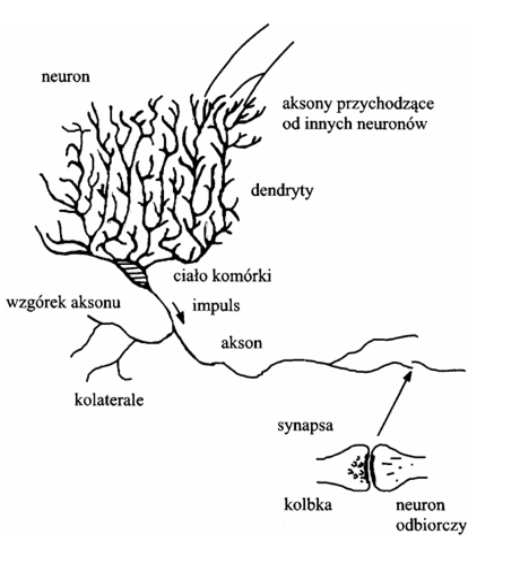
\includegraphics[resolution=100, scale=0.7]{neuronMozgowy.png}
		\caption{Wizualizacja uproszczonego modelu neuronu mózgowego.}
\end{figure}

\begin{figure}[ht]
	\centering
			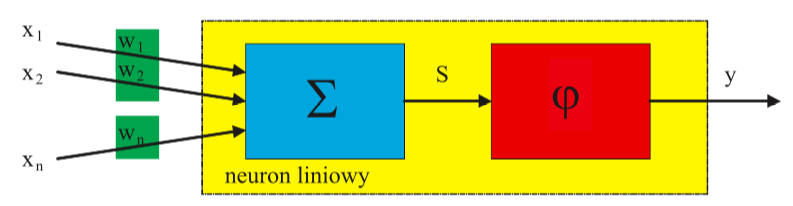
\includegraphics[resolution=100, scale=0.68]{sztucznyNeuron.png}
		\caption{Wizualizacja prostego sztucznego neuronu.}
\end{figure}

Model obliczeniowy został stworzony na podstawie algorytmu logiki progowej. 
Nazwa neuronu sztucznego została przyjęta w kręgach akademickich i biznesowych, stąd często osoby nie znające budowy mózgu ani działania sieci neuronowych mylnie nazywają zagadnienie Sztuczną Inteligencją, uproszczając skomplikowane procesy biologiczne do wzmacniania lub osłabiania sygnałów przekazywanych przez synapsy. Sieci neuronowe naśladują tylko jeden rodzaj pamięci, pamięć deklaratywną i w odosobnieniu nie tworzy inteligencji.

\section{Model perceptronu prostego}
Podstawowym elementem z których buduje się sieci neuronowe są sztuczne neurony, nazywane również perceptronami. Mają one być w rzeczywistości bardzo uproszczonym odwzorowaniem komórek nerwowych występujących w mózgu. Takie uproszczenia pozwalają na łatwą implementację modelu matematycznego, który ma reprezentować nasz obiekt i być tani w replikacji. Nawet po takim uproszczeniu jest on w stanie skutecznie naśladować ''uczenie''.
Sztuczny neuron jest funkcją matematyczną $$f(x,w) \to y$$. Można go opisać za pomocą modelu złożonego z:
\begin{itemize}
\item określonej liczby wejść \(n \in \mathbb{N}\),
\item wagi, skojarzonej z każdym z wejść \(w_i \in \mathbb{R}, i=1..n\),
\item wybranej funkcji aktywacji \(\phi: \mathbb{R} \to \mathbb{R} \)
\end{itemize}

Charakterystycznym elementem budulca sieci jest wiele wejść i tylko jedno wyjście, dlatego tak łatwo stworzyć model będący funkcją matematyczną.
Dane wejściowe oraz wyjściowe mogą przyjmować wartości z ograniczonego przedziału. Wartości przekazywane na wejściu i wartość wyjściowa zazwyczaj przyjmują znormalizowane wartości z przedziału \(x \in [-1, 1]\) dla każdego z wejść, oraz \(y \in [-1,1]\) dla wyjścia. W uproszczeniu można przyjąć \(y = \sum\limits_{i=1}^n (w_i * x_i)\). \(w_i\) są nazywane wagami (dawniej wagami synaptycznymi) i podlegają zmianom w trakcie uczenia neuronu. Wagi stanowią zasadniczą cechę sieci neuronowych działających jako adapcyjne systemy przetwarzania informacji. Zsumowana wartość jest wejściem dla funkcji aktywacji neuronu. Funkcja aktywacji zwyczajowo ma kształt sigmoidy, ale stosowane są obecnie również funkcje nazywane rektyfikowanymi jednostkami liniowymi. Funkcja progowa ma za zadanie symulację zachowania przekaźnika synapsy, po przekroczeniu określonego progu aktywuje się dane zachowanie lub jak na przykładzie obrazów rozpoznanie cechy.

Ta prosta jednostka stanowi dziś podstawę budowy każdej sieci neuronowej. Aby funkcja zwracała oczekiwane wyniki, wagi powinny być poprawnie ustawione. Początkowo wagi ustawiano ręcznie za pomocą operatora (osoby przełączającej fizyczne kable), który wcześniej przeliczał je dla odpowiednich parametrów wejścia\\wyjścia. W latach 50tych perceptron stał się pierwszym modelem umiejącym samodzielnie wyliczyć poprawnie wagi definiujące zadaną klasę na podstawie przykładów. Wagi w zależności od wartości mogą sygnał wejściowy wzmocnić gdy waga jest większa od 1, lub stłumić gdy waga jest mniejsza niż 1. To pozwala wyuczonemu już perceptronowi na porównanie cechy obiektu wejściowego z tym co potrafi rozpoznać.

W jaki sposób sztuczny neuron jest w stanie rozpoznać sygnał wejściowy? Do wyjaśnienia zjawiska w literaturze zazwyczaj prezentuje się przedstawienie modelu w notacji wektorowej.
\newline
\(X = \begin{bmatrix} x_{1} \\ x_{2} \\ \dots \\ x_{n} \end{bmatrix} \) - wektor wyznaczający przestrzeń wejść, oraz \newline
\(W = \begin{bmatrix} w_{1} \\ w_{2} \\ \dots \\ w_{n} \end{bmatrix} \) - wektor wyznaczający przestrzeń wag. \newline W ten notacji można wyrazić wyjście neuronu jako \(y= W^T * X\). Wartość wyjściowa neuronu y, będzie wyższa im bliższe będzie położenie wektorów. \cite{sieciNeuronowe}

\begin{figure}[ht]
	\centering
			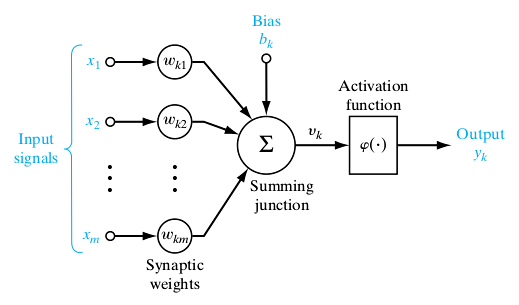
\includegraphics[resolution=100, scale=0.7]{Neuron.png}
		\caption{Prosta reprezentacja neuronu.}
\end{figure}

\section{Co to jest sieć neuronowa?}
Koncepcja sztucznej sieci neuronowej to połączenie wielu neuronów w jeden obiekt. Pozwala to na rozpoznawanie bardziej skomplikowanych wzorców i większej różnorodności typów obiektów niż klasyfikacja binarna. Zwykła (płytka) sieć neuronowa składa się z trzech warstw węzłów. Warstwa pierwsza stanowi warstwę wejściową sieci i składa się z sygnału wejściowego.

Kolejna warstwa jest nazywana warstwą ukrytą, użytkownik nie ma dostępu do niej, przypomina czarną skrzynkę. Nie można zaobserwować co się wewnątrz niej dzieje, użytkownik widzi jakie są dane wejściowe, wartości które powinny zostać zwrócone (w ostatniej warstwie), ale nie ma informacji co jest i powinno się znajdować w tej warstwie podczas trenowania sieci.
Ostatnia warstwa, pojedynczy węzeł nazywany jest warstwą wyjściową. Pobiera wektor wartości wyjściowych z poprzedniej warstwy (ukrytej) i na nim zostaje obliczona wartość wyjściowa (odpowiedź).

Taka architektura nazywa się siecią dwuwarstwową. Dane wejściowe, mimo że tworzą pierwszą warstwę nie są liczone w nazewnictwie.
Z warstwami ukrytą i wyjściową powiązane są parametry \(w\) (ang. weight) oraz \(b\) (ang. bias), oznaczające kolejno: macierz wag oraz wektor progów.

\begin{figure}[ht]
	\centering
			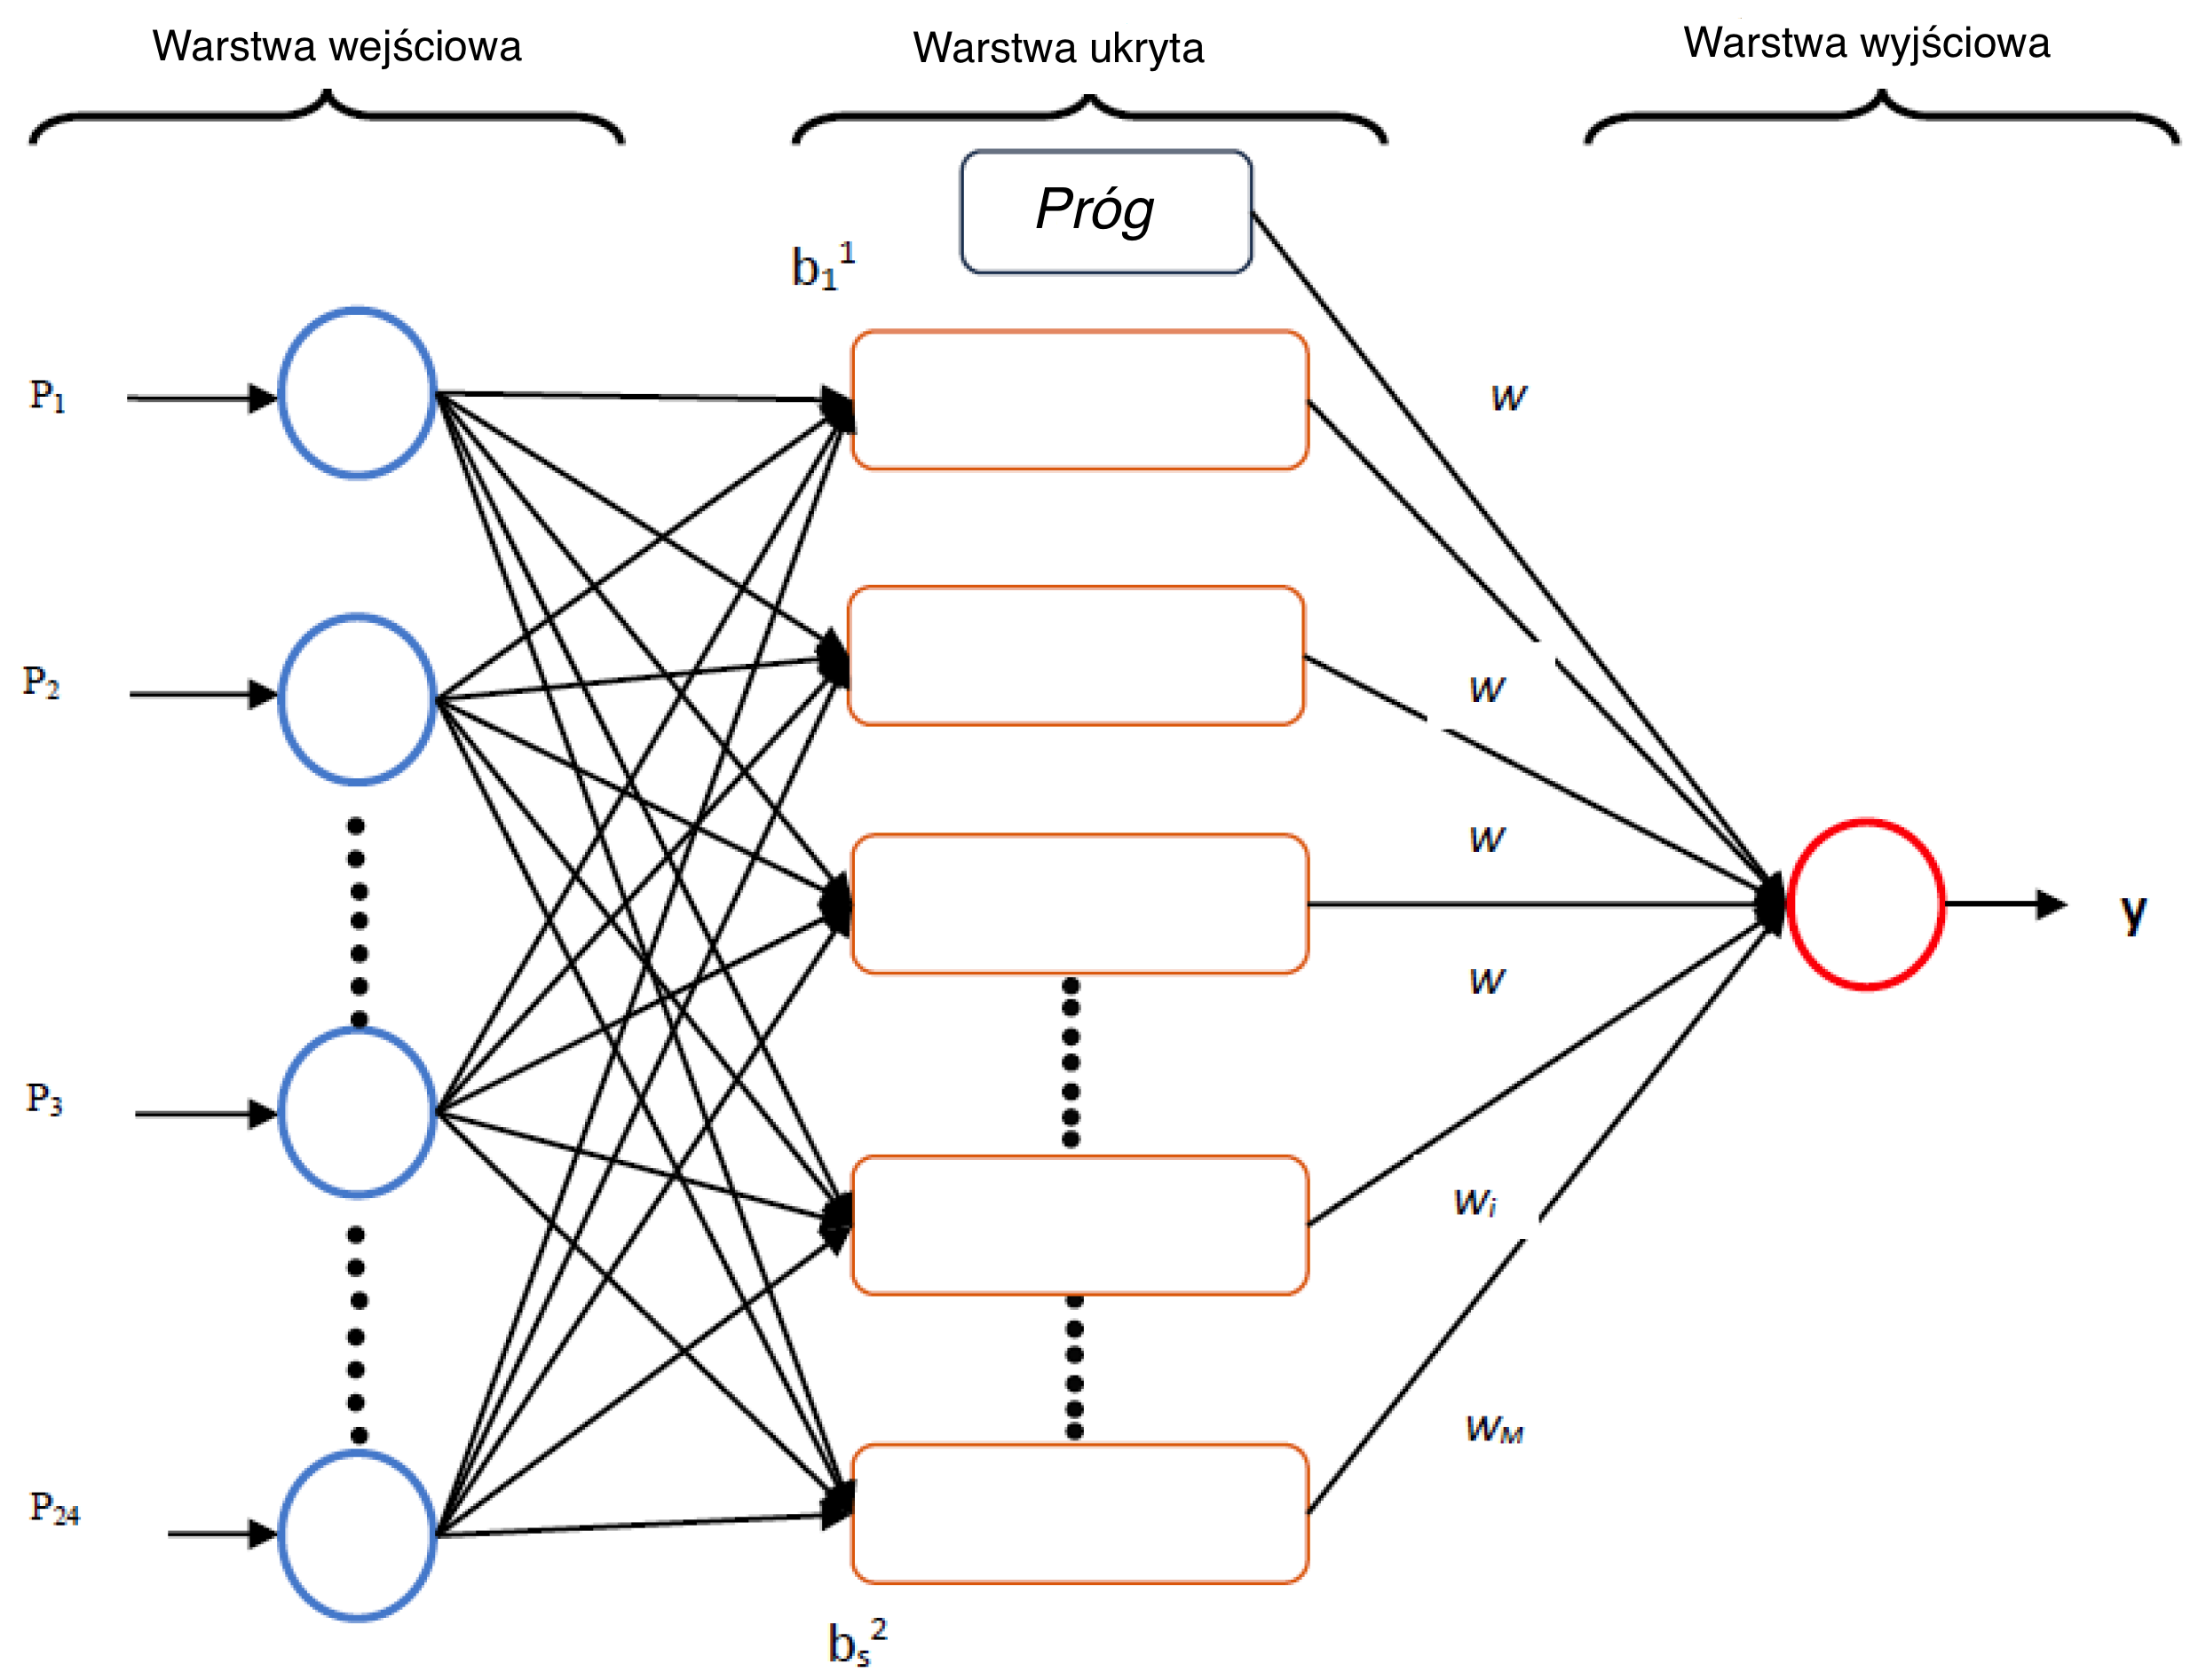
\includegraphics[resolution=100, scale=0.2]{SiecNeuronowa.png}
		\caption{Prosta sieć neuronowa złożona z dwóch warstw.}
\end{figure}

\section{Jak uczyć sieci neuronowe}
W obecnym momencie istnieją dwie możliwości by sieć posiadła umiejętność poprawnej klasyfikacji. Można wyznaczyć dla algorytmu zbiór opisanych sygnałów wejściowych wraz z oczekiwanym sygnałem wyjściowym, ten typ tworzenia modelu sieci jest uczeniem nadzorowanym, co jest szczegółowo omawiane w tej pracy. Drugim podejściem jest podanie sygnałów wejściowych bez opisów i oczekiwanych wartości wyjściowych, to podejście nazywa się uczeniem nienadzorowanym.

\subsection*{Uczenie nadzorowane}
Jest to typ uczenia maszynowego, które zakłada obecność ludzkiego nauczyciela. Nauczyciel zobowiązany jest stworzyć odpowiednie dane uczące. Takie dane są parą danych, wejściowego obiektu uczącego oraz prawidłową odpowiedź wyjściową do tej danej. System na podstawie tych danych ma nauczyć się przewidywać poprawną odpowiedź dla nowych danych, ze znanej mu domeny.

Zadania uczenie nadzorowanego dzielą się na dwie kategorie, regresję i klasyfikację. 

W problemie regresji próbuje się przewidzieć wyniki, które są wartościami ciągłymi, czyli mając jakieś dane próbuje się je mapować na funkcję ciągłą. 

W problemie klasyfikacji algorytm ma za zadanie przewidzieć wyniki będące wartościami dyskretnymi, uściślając jest to znajdowanie klas obiektów, na podstawie danych wejściowych. \cite{Gron:2017:HML:3153997}

Uczenie nadzorowane ma wiele zastosowań, do głównych należą (wraz z używanym typem sieci):
\begin{itemize}
\item przewidywanie cen nieruchomości (zwykła sieć neuronowa),
\item reklamy internetowe (zwykła sieć neuronowa),
\item rozpoznawanie mowy (rekurencyjna sieć neuronowa),
\item tłumaczenie maszynowe w translatorach (rekurencyjna sieć neuronowa),
\item samochody autonomiczne (sieci hybrydowe lub inne niestandardowe sieci),
\item rozpoznawanie obiektów na obrazach (konwolucyjna sieć neuronowa).
\end{itemize}
Ostatnie z wyżej wymienionych zastosowań jest tematem badanym w tej pracy.

Uczenie nadzorowane dzieli się również binarnie ze względu na strukturę dostarczonych danych. Pierwszy rodzaj danych, dane zawierające konkretną strukturę, zazwyczaj tabela, są bardzo dobrze obsługiwane przez większość znanych wcześniej algorytmów uczenia maszynowego i nie wymagają ogromnej mocy obliczeniowej. Choć sieci neuronowe świetnie się sprawdzają przy tego typu danych, używanie ich ma sens dopiero gdy danych jest bardzo dużo (wielkość tabel przekraczające miliony rekordów). Drugi typ danych, nieustrukturyzowane zdjęcia, pliki audio, tekst, jest znacznie trudniejszy do rozpoznania przez komputer, za to dużo bardziej naturalny dla ludzi. Dzięki głębokim sieciom neuronowym i wielkiej mocy obliczeniowej komputerów, dokładność algorytmów uczących się na tego typu danych znacząco wzrosła, z 70\% do ok 95-99\% dokładności zależnie od ilości danych.

\subsection*{Uczenie nienadzorowane}
Uczenie maszynowe bez nadzoru nauczyciela jest drugim typem uczenia maszynowego polegającym na wyciąganiu wniosków z danych bez informacji zwrotnej o poprawności wniosków oraz bez określania etykiety danych. W algorytmach tego typu nie ma funkcji wyznaczającej poprawność utworzonego modelu. Najczęstszym zadaniem stawianym algorytmom uczenia nienadzorowanego jest wyznaczanie klastrów ze zbioru danych. W tej pracy temat uczenia bez nauczyciela nie jest poruszany.

\section{Elementy sieci neuronowych} 
Sieci neuronowe do poprawnego działania potrzebują więcej niż tylko połączenia ze sobą neuronów. Należy dobrać odpowiednie algorytmy korygujące błędy. Aby algorytm zatrzymał się w odpowiednim momencie z osobna trzeba zdefiniować warunki stopu dla epoki, ilość epok, rozmiar danych. Każda warstwa musi posiadać określoną funkcję aktywacji. Ostatnim opisanym elementem sieci są hiperparametry, czyli właściwości sterujące algorytmem by wiedział w jaki sposób wyznaczać pozostałe parametry.

\subsection{Metoda gradientu prostego}
Algorytm stosowany do szukania minimum lokalnego płaszczyzny wyznaczonej funkcją. Jest to bardzo prosta metoda optymalizacji stosowana do wyznaczania wag i progów. Płaszczyzna złożona z osi poziomych \(w\) i \(b\) oraz oś pionowa będąca wartością funkcji kosztu \(J(w,b)\). Algorytm mając początkowo losowe wagi i progi, rozpoczyna w tym losowym miejscu sprawdza wartość funkcji kosztu, następnie wykonuje małe przesunięcie w najbardziej stromym kierunku w dół płaszczyzny. Operacja zejścia powtarzana jest do znalezienia do minimum lokalnego.

\begin{algorithm}
i = 0\;
\While{i \textless x}{
	\(w = w - \alpha * \frac{\partial J(w,b)}{\partial w}\)\;
	\(b = b - \alpha * \frac{\partial J(w,b)}{\partial b}\)\;
	\(i++\)\;
}
\caption{Schemat algorytmu}
\end{algorithm}

\subsection{Funkcje aktywacji}
Budując sieć neuronową należy zdefiniować funkcje aktywacji dla warstw ukrytych oraz warstwy wyjściowej. Funkcje aktywacji znane są również jako charakterystyka neuronu. Charakterystyka neuronu jest elementem, który pośredniczy między zsumowanym pobudzeniem neuronu, a jego danymi wejściowymi. 

Najczęściej używaną charakterystyką była do niedawna funkcja sigmoidalna ponieważ ma wiele zalet:
\begin{itemize}
\item zapewnia łagodny gradient między wartościami 0 a 1,
\item ma gładką i prostą do liczenia pochodną,
\item jednym parametrem można dobrać kształt krzywej.
\end{itemize}
Definicja funkcji sigmoidalnej \(f(x) = \frac{1}{1+e^{-z}}\).
Obecnie nie jest zalecane używanie funkcji sigmoidalnej poza przypadkami na warstwie wyjściowej w przypadku klasyfikacji binarnej, kiedy należy stwierdzić prawdopodobieństwo klasy obiektu. Dużo wydajniejszym odpowiednikiem jest następna funkcja.

Sprawną funkcją aktywacji jest tangens hiperboliczny. Jego wartości zawierają się między -1 i 1. Definicja funkcji tangensu hiperbolicznego \(tanh(x) = \frac{e^{x} - e^{-x}}{e^{x} + e^{-x}}\). Jak widać na załączonych rysunkach ta funkcja jest przesunięciem sigmoidy względem osi y, tak że przechodzi przez punkt \((0,0)\). Dla warstw ukrytych charakterystyka neuronu będąca tangensem hiperbolicznym ma lepszą skuteczność. Mediana wartości wychodzących z warstw ukrytych wynosi 0. Nie trzeba wtedy stosować skalowania względem sigmoidy, co znacząco ułatwia uczenie.

Zalecaną charakterystyką neuronu w dużych architekturach jest rektyfikowana jednostka liniowa. Stała się ona domyślną funkcją stosowaną w bibliotekach implementujących sieci neuronowe. Funkcja zwraca przekształecenie nieliniowe. Na rysunku widać że funkcja bardzo przypomina liniową, składa się z dwóch liniowych fragmentów. To jest jedna z największa zalet, ponieważ funkcja ta jest banalna w implementacji i wyliczeniu wartości. Definicja funkcji jest w porównaniu do pozostałych jest banalna \(relu(z) = max(0,z)\). Jedynym problemem przy używaniu ReLU jest wyliczenie pochodnej kiedy argument z jest mniejszy od 0. W praktyce nie sprawia to większych problemów bo wartość zostanie ustawiona na 0, ale opracowano funkcję która jest pozbawiona tej niedogodności.

Nieszczelna liniowa jednostka rektyfikowana (ang. leaky Rectified Linear Unit) definiowana \(f(x) = max(x, 0.01x)\). Pozwala to zmniejszyć efekt kiedy pochyła funkcji schodzi do 0, spowalniając uczenie. Niestety ta funkcja nie jest powszechnie używana w praktyce.

Należy podkreślić że w nowoczesnych sieciach neuronowych każda warstwa może posiadać indywidualnie ustanowioną funkcję aktywacji w zależności od architektury. Domyślnym wyborem funkcji aktywacji jest ReLU. 

\begin{figure}[ht]
	\centering
			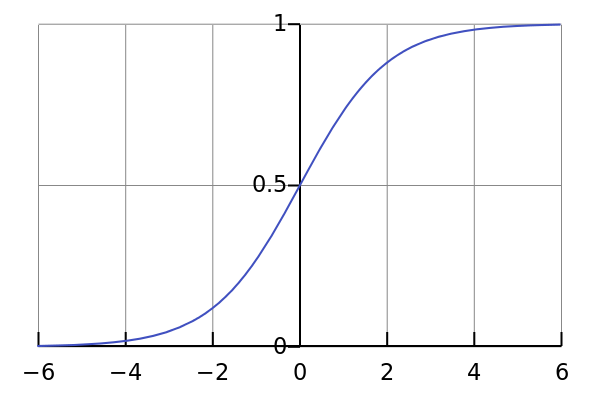
\includegraphics[resolution=100, scale=0.7]{Sigmoid.png}
		\caption{Wykres funkcji sigmoidalnej}
\end{figure}

\begin{figure}[ht]
	\centering
			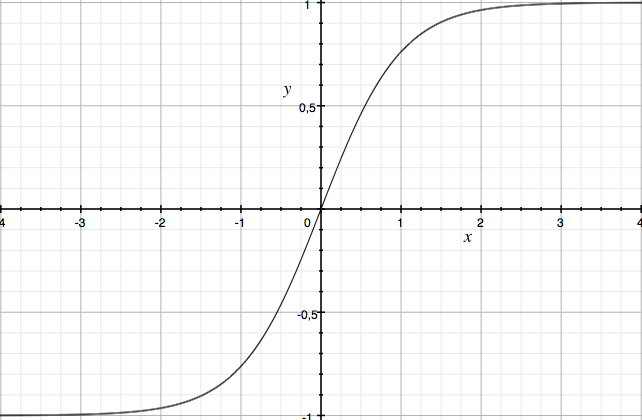
\includegraphics[resolution=100, scale=0.7]{Tangens.png}
		\caption{Wykres funkcji tangensu hiperbolicznego}
\end{figure}

\begin{figure}[ht]
	\centering
			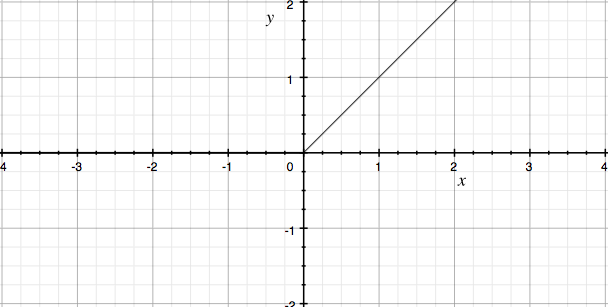
\includegraphics[resolution=100, scale=0.8]{ReLU.png}
		\caption{Wykres rektyfikowanej jednostki liniowej}
\end{figure}

\begin{figure}[ht]
	\centering
			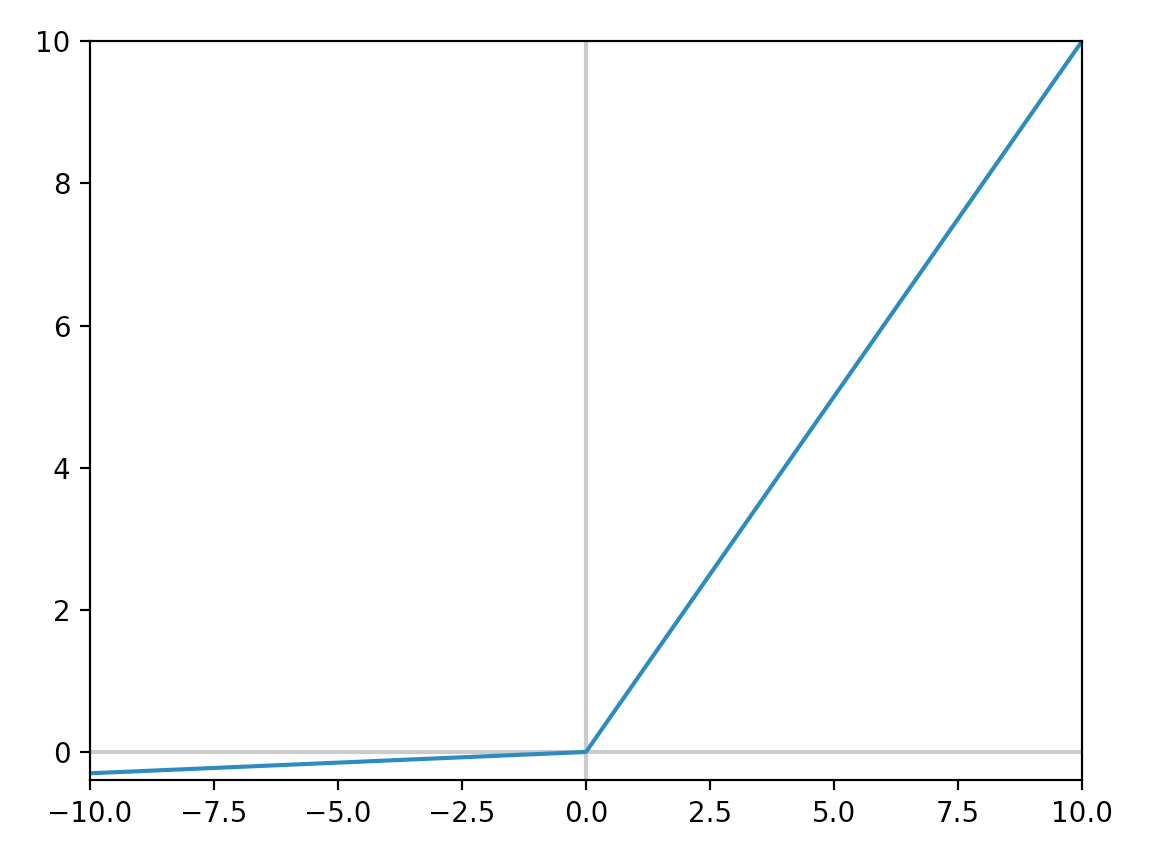
\includegraphics[resolution=100, scale=0.8]{leakyReLU.png}
		\caption{Wykres nieszczelnej rektyfikowanej jednostki liniowej}
\end{figure}

\subsection{Parametry}
Najważniejszy element sieci neuronowej. Składa się na niego zbiór wag i progów (bias). Wagi wyznaczają sposób działania sieci, która ma nauczyć się dobrać odpowiednie parametry przy pomocy algorytmu uczącego, odpowiednio dobranych hiperparametrów oraz zbioru danych uczących. Wagi muszą być dobrane w sposób umożliwiający neuronom wykonanie czynności, których się od nich wymaga. Ze względu na ilość wag w głębokich sieciach, gdzie dla każdego z tysięcy neuronów może istnieć kilkaset wejść, proces musi być automatyczny. Sieć musi wiedzieć kiedy każdy z neuronów zwiększa swoją dokładność czy nie. Wagi i progi powinny być elastyczne i zmieniać się bardo szybko na początku procesu uczenia i tylko w niewielkim stopniu zmieniać wartości kiedy algorytm kończy proces uczenia.

\subsection{Hiperparametry}
Tworzenie dobrej sieci neuronowej wymaga nie tylko parametrów ale również rozważnego doboru hiperparametrów. Elementy ''ręcznie'' dobierane dla algorytmu uczenia. Najczęściej ustawiane parametry dla sieci neuronowej to:
\begin{itemize}
\item stała uczenia,
\item ilość iteracji uczenia w jednej epoce,
\item ilość ukrytych warstw,
\item ilość ukrytych jednostek,
\item wybór funkcji aktywacji (ReLU, tangens, sigmoida),
\item parametry regularyzacji,
\item rozmiary próbek uczących,
\end{itemize}
i wiele innych mniej ważnych hiperparametrów.

Są to parametry kontrolujące sposób wykonania algorytmu uczącego i w ostateczności to one mają największy wpływ na skuteczność uczenia parametrów wag oraz progów (ang. bias). Nie ma na chwilę obecną dobrego przewodnika w jaki sposób dobierać hiperparametry. Zwyczajowo stosuje się metodę prób i błędów na podstawie tego jak algorytm się zachowuje. \cite{sitefastAI} Za każdą zmianą wartości należy uruchomić algorytm i sprawdzić jak zachowuje się funkcja kosztu, jeśli maleje lepiej niż przy poprzednich wartościach można stroić dalej w tym kierunku. Dopieranie odpowiednich wartości niestety jest procesem empirycznym i należy wyrobić odpowiednią intuicję aby jak najtrafniej dobierać parametry od początku. Wartości te też nie są stałe, zmieniają się w zależności od dziedziny badanego zagadnienia. Być może najbliższe lata przyniosą dobry i spójny przewodnik dobierania najlepszych wartości, pozwoli to znacznie zautomatyzować proces.

\subsection{Wykres obliczeniowy}
Aby opisać organizację obliczeń podsekcję o wstecznej propagacji błędu, należy sformalizować operacje obliczeń. Robi się to za pomocą wykresu obliczeniowego. Węzły w grafie reprezentują skalary, wektory, macierze i tensory. Drugim elementem w grafie są operacje czyli proste funkcje z jedną lub większą ilością zmiennych. Graf obliczeniowy przydaje się kiedy istnieje zdefiniowana funkcja bądź zmienna, którą należy zoptymalizować, w przypadku sieci neuronowych oczywistą jest funkcja kosztu.

Dla przykładu chcę obliczyć funkcję kosztu \(J\) o zmiennych \(a,b,c\) zdefiniowaną \(J(a,b,c) = 3(a+bc)\). Obliczenie tej funkcji składa się z trzech kroków, pierwszym jest policzenie \(b*c\).
$$i = b * c$$
Następnym krokiem jest dodanie zmiennej a.
$$k = a + i$$
Trzecim i ostatnim krokiem jest wyjście funkcji kosztu \(J = 3k\).
Graf obliczeniowy powyższej funkcji znajduje się na rysunku poniżej.

Do minimalizowania funkcji kosztu algorytm oblicza pochodne w odwrotnej kolejności do przedstawionej na poprzednim przykładzie grafu.

\begin{figure}[ht]
	\centering
			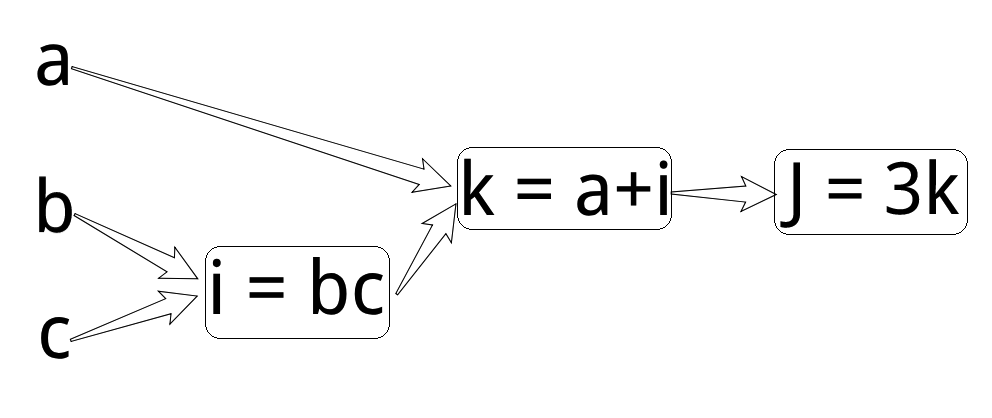
\includegraphics[resolution=100, scale=0.4]{ComputationGraph.png}
		\caption{Wykres obliczeniowy dla funkcji \(J(a,b,c) = 3(a+bc)\)}
\end{figure}

\subsection{Wsteczna propagacja błędu}
Algorytm wstecznej propagacji błędu został opracowany w latach 70tych, jednak używany dopiero ponad 10 lat później kiedy Rumelhart, Hinton i Williams wykazali skuteczność metody w strojeniu wag w ukrytych warstwach sieci.

Przekazując sygnał na wejście sieci zostaje on propagowany w przód przez wszystkie warstwy do warstwy wyjściowej. Losowy neuron w warstwie ukrytej otrzymuje wartości wyjściowe z neuronów poprzedniej warstwy, mnoży każdy otrzymany sygnał z wagą przypisaną danemu wejściu i przekazuje zsumowany wynik do funkcji aktywacji. Każdy neuron wykonuje takie operacje do czasu trafienia na ostatnią warstwę gdzie sieć podaje juz oczekiwany wynik. Cały ten proces nazywa się propagacją w przód. Mając oczekiwany wynik na warstwie wyjściowej, zazwyczaj prawdopodobieństwo przynależności do każdej z uczonych klas należy wyliczyć funkcję błędu (ang. loss function). Funkcja ta pozwala określać odchylenie wyliczonego wyniku od właściwej odpowiedzi. Celem sieci jest zminimalizowanie błędu przez wyliczenie pochodnej z funkcji kosztu w stosunku do wag modelu.

Wsteczna propagacja błędu jest narzędziem używanym przez algorytm gradientu spadkowego aby wyliczyć gradient funkcji błędu. W trakcie przejścia wstecz przez sieć neuronową następuje korekcja wag. Przechodząc od wartości wyjściowej należy zmodyfikować wagi warstwy poprzedzającej tak by zmniejszyć wartość funkcji błędu.

Istnieją również analogiczne metod korekcji wag, jak szybka propagacja (ang. quick-propagation) oraz bardziej skomplikowane i ograniczone założeniami matematycznymi metoda gradientów sprzężonych i metoda Levenberga-Marquardta. Metody te są dużo szybsze od wstecznej propagacji błędu, ale przez swoje ograniczenia prawie nigdy nie są używane w praktyce. \cite{odkrywanieSieci}

%\subsection{Jak zbudować sieć neuronową}

% ################################
%        DEEP LEARNING
% ################################

\chapter{Głębokie sieci neuronowe}
%\section{Tworzenie głębokich sieci}
W tym rozdziale zostały przybliżone trzy interesujące techniki głębokiego uczenia. Zostały wybrane ze względu na ich obszerną ilość zastosowań oraz potencjał, który można wykorzystać przy rozpoznawaniu wzorców na obrazach. Jedna z nich zostanie używana wielokrotnie w dalszej części pracy, jest w szczególności istotna ze względu na wykorzystanie w rozpoznawaniu obrazów. Wszystkie opisywane architektury korzystają z konwolucyjnych sieci neuronowych.
\section{Zmiany na przestrzeni lat}
Podstawowe techniki znane z głębokiego uczenia znane są już od dziesięcioleci, należy teraz odpowiedzieć na pytanie dlaczego dopiero teraz zostają wykorzystane na masową skalę przez wszystkie firmy technologiczne, a powoli także przemysłowe. Sieci neuronowe z powodzeniem były wykorzystywane do prostych zadań jak rozpoznawanie cyfr, kodów kreskowych, kodów pocztowych, pisma odręcznego od wczesnych lat 90tych ubiegłego wieku. Ze względu na ograniczenia wydajnościowe komputerów osobistych i brak odpowiedniej architektury przetwarzania obliczeń równoległych modele wyprodukowane przez sieć musiały być bardzo małe, tak małe żeby mieściły się na dysku twardym o pojemności mniejszej niż płyta DVD. Wytrenowanie modelu, który jest przechowywany na dysku, zamiast pamięci podręcznej, bądź jak obecnie w jeszcze szybszej pamięci karty graficznej, jest zadaniem tak czasochłonnym, że nie opłacało się tworzyć głębokich sieci neuronowych z tysiącami parametrów na komputerach klasy PC. Wynalezienie osobnego procesora do zadań graficznych i jego późniejsze możliwości programowania na specjalistycznym SDK umożliwiły eksperymenty z głębokim uczeniem w czasie iteracji liczonym w tygodniach, nie miesiącach. Wydajność obliczeniowa procesorów GPU znalazła się na odpowiednim poziomie dopiero po roku 2010. Jak opisano w pracy, jeszcze w 2012 roku wytrenowanie sieci AlexNet zajęło dwa tygodnie na dwóch kartach NVIDIA GeForce 580 GTX, najmocniejszych na tamtą chwilę na rynku dla graczy. NVIDIA na swoim blogu chwali się informacjami jakoby przyspieszenie kart graficznych między latami 2012 a 2015 wzrosło pięćdziesięciokrotnie. \cite{siteNvidiaAcceleration} Drugim równie ważnym aspektem nagłego rozkwitu w rozwoju głębokich sieci jest ilość dostępnych danych. Smartfony umożliwiły generowanie danych tekstowych, dźwiękowych i miliardów gigabajtów zdjęć i filmów. Taka ilość danych idealnie współgra z rosnącą wydajnością sieci neuronowych. Innowacje w zakresie algorytmów odbyły w zakresie optymalizacji szybkości obliczeń. Jednym z głównych przykładów zwiększenia wydajności jest przejście z funkcji sigmoidy jako funkcji aktywacji do funkcji ReLU. Ta funkcja liczy się dużo szybciej, ponieważ dla wszystkich dodatnich wartości, nachylenie gradientu wynosi 1, w sigmoidzie zaś gdy wartość często wynosi 0, parametry zmieniają się dużo wolniej.

Innowacje dzieją się dużo szybciej kiedy cykl iteracyjny od pomysłu, przez kod do eksperymentu dzieje się prawie w czasie rzeczywistym, w przeciwieństwie do wcześniejszych możliwości gdy trening trwał często ponad miesiąc. Głębokie uczenie jeszcze większych sieci przyspieszy z ciągłym strumieniem nowych, opisanych danych, oraz coraz to szybszym sprzętem.

\section{Głębokie sieci neuronowe}
Elementy sztucznych sieci neuronowych zostały opisane w poprzednim rozdziale, w tej sekcji uwaga skupiona jest na podziale architektur, głębokości warstw ukrytych oraz rodzajach dodatkowych warstw, takich jak filtr cech, warstwy łączące, konwolucje.

Głębokie sieci neuronowe znane są również jako sieci neuronowe typu \textit{feedforward} (w literaturze autor nie znalazł polskiego odpowiednika na to słowo, również prof. Tadeusiewicz posługuje się angielską nazwą), kolejna nazwa to wielowarstwowy perceptron. Nazwa \textbf{feedforward} ma naznaczyć że wszystkie informacje przepływają przez funkcję wyliczaną z \(x\), przez pośrednie operacje wyliczające \(f\) by ostatecznie trafić do wyjścia \(y\). Przez brak informacji zwrotnej, która mogłaby natychmiast przekazać neuronowi wyliczone wartości. W przypadku jeśli sieć neuronowa ma otrzymywać natychmiastową informację zwrotną tworzona jest rekurencyjna sieć neuronowa przedstawiana w jednej z sekcji tego rozdziału. Wszystkie wymienione określenia opisują sieć której zadaniem jest przybliżyć funkcję \(f*\). Klasyfikator \(y = f*(x) \) mapuje wejście \(x\) do kategorii \(y\). Wielowarstwowy perceptron definiuje mapowanie \(y = f(x,\theta)\) ucząc się parametrów \(\theta\), w sposób pozwalający wydobyć jak najlepsze przybliżenie funkcji. Przykłady uczące serwowane sieci dają przybliżony obraz jak ma wyglądać funkcja. W typowej sieci, funkcji aktywacji jest wiele i są one wywoływane jednak przez drugą, taki łańcuch funkcji pozwala określać głębokość wybranej sieci (stąd ich nazwa "głębokie sieci neuronowe"). Dokładanie kolejnych warstw można urozmaicić przez wybieranie innego typu jednostek dla każdej z warstw, co może ulepszyć jakość architektury. O skuteczności takich rozwiązań traktuje rozdział poświęcony porównaniu efektywnych architektur. Ten rodzaj sieci jest najbardziej użyteczny do zastosowań przetwarzania obrazów i jego modyfikacje będą opisane w dalszej części pracy.

\begin{figure}[ht]
	\centering
			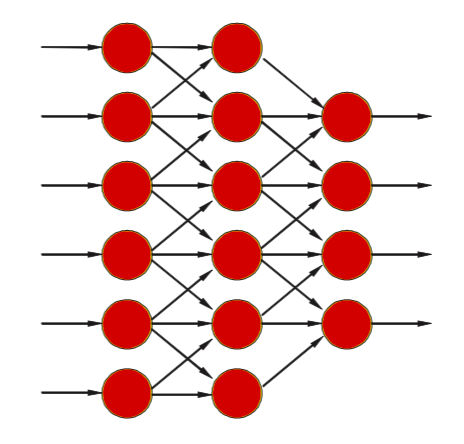
\includegraphics[resolution=100, scale=0.6]{feedforwardNetwork.png}
		\caption{Przykładowa struktura sieci typu feedforward.}
\end{figure}

Każda sieć która ma więcej niż jedna warstwę ukrytą ma prawo być nazwana głęboką, jednak im sieć jest głębsza tym lepsze potrafi osiągnąć wyniki. Warstwy ukryte działają bez możliwości wglądu w nie w trakcie uczenia, programista, nie ma również kontroli nad informacjami przekazywanymi między warstwami ukrytymi.

Możliwości uczenia wielowarstwowych sieci neuronowych, sprawiają że są one idealnymi kandydatkami na zadania wymagające rozpoznawania obrazów. Używając zwykłej sieci typu feedforward, cechy obrazu zostają wyodrębnione przez ekstraktor w trakcie działania algorytmu (strojenie parametrów) a pozostałe informacje są odrzucane. Klasyfikator następnie dzieli na kategorie wektory z wyodrębnionymi cechami obrazu. Ta metoda jest skuteczna dla sieci w pełni połączonych ze sobą, jednak niesie ze sobą poważny problem uniemożliwiający stosowanie jej obecnie na większą skalę.

Zdjęcia są duże i ich rozmiar wraz z nowymi smartfonami rośnie dużo szybciej niż przepustowość kart graficznych. Taka sieć wymagałaby już tysięcy ukrytych jednostek w pierwszej warstwie ukrytej, co daje setki tysięcy lub miliony parametrów tylko na pierwszej warstwie. Mając obraz o niewielkiej rozdzielczości 250 x 250 x 3, pełne połączenie warstwy wejściowej z pierwszą ukrytą warstwą wielkości 100 000 neuronów, wygeneruje 18 750 000 000 parametrów już w pierwszej warstwie. Obecne sieci z ponad czterdziestoma warstwami stały by się zbyt wielkie na jakikolwiek komputer czy chmurę obliczeneiową. Większe możliwości sieci kosztem zapotrzebowania na moc przetwarzania dostarczanych przez nie danych, pozostają poza zasięgiem większości osób i podmiotów. W pełni połączona sieć wymaga większej ilości reprezentacji (przykładów uczących) dla każdej klasy, ponieważ nie ma ona informacji o przesunięciach, różnych kątach, pochyleniu. Takie dane należałoby wygenerować automatycznie lub znaleźć wielokrotnie większy zbiór etykietowanych obrazów.

Drugą poważną wadą tej architektury jest ignorowanie ułożenia lokalnego sygnału wejściowego. Zdjęcie można w dowolny sposób poszatkować, pomieszać a wyjście pozostanie takie samo. Niestety w przypadku rozpoznania obiektu na zdjęciach jest to nie do przyjęcia. Rozwiązaniem tych problemów jest kolejny typ sieci wywodzący się z wielowarstwowego perceptronu, konwolucyjna sieć neuronowa  (ang. Convolutional Neural Network).

\section{Konwolucyjne sieci neuronowe}
Wyspecjalizowany typ sieci neuronowych do przetwarzania danych ułożonych w siatkę. Sieci te są niezwykle skuteczne w przetwarzaniu siatek pikseli i nowoczesne sieci splotowe zakładają użycie wyłącznie obrazów i posiadają wbudowane optymalizacje dla tego typu sygnałów. Sieci te nie odbiegają znacząco od klasycznych feedforward'owych. Ich dodatkową cechą jest jak wynika z nazwy, liniowa operacja konwolucji (splotu) matematycznej. Wraz z konwolucją dochodzi wymagana operacja łączenia (ang. pooling).  W sieciach konwolucyjnych łączy się trzy narzędzia, lokalne pola percepcji, współdzielenie wag, przestrzenne lub czasowe próbkowanie. Te narzędzia rozwiązują również trzy problemy, przesunięcie, skalowanie i zniekształcenie obrazu.

Prosta i zwykła sieć konwolucyjna otrzymuje na wejściu obrazy o znormalizowanej wielkości i w miarę możliwości wycentrowane. Każdy neuron w wybranej warstwie otrzymuje wejście ze zbioru neuronów z poprzedniej warstwy, które znajdują się w jego sąsiedztwie. Połączenia lokalne były wielokrotnie używane w modelach uczenia maszynowego. Używając lokalnych pól recepcyjnych, jednostki są w stanie wyodrębnić pojedyncze cechy obrazu takie jak krzywizny, krańce płaszczyzn. Cechy te są przekazywane w grupach do kolejnych warstw, gdzie tworzy się z nich coraz wyższe poziomy abstrakcji obiektu, by w ostatniej warstwie nadać im już konkretny kształt obiektu. Zastosowanie warstw rozpoznających najbardziej podstawowe cechy, pozwala używać jednego neuronu do rozpoznania wielu części obrazu jeśli obiektów występuje więcej. Neurony wybranej warstwy zorganizowane są na płaszczyźnie, w której wszystkie jednostki dzielą zestaw wag. Zbiór wartości wyjściowych neuronów zadanej płaszczyzny jest nazywany mapą cech. Jednostki w mapie cech wykonują tę samą operację na różnych fragmentach zdjęcia. Warstwa konwolucyjna zatem jest złożona z wielu map cech, aby zebrać wiele cech w różnych miejscach obrazu. Jednostka w mapie cech ma połączone wejścia z polem recepcyjnym o mniejszym rozmiarze.

Na końcu sieci splotowej architektura zredukuje cały obraz do pojedynczego wektora z wynikami prawdopodobieństwa klas ułożonych wgłąb.

Lokalność cech polega na zebraniu neuronów obecnej warstwy będących w sąsiedztwie ze sobą i przekazaniu ich wartości do neuronu kolejnej warstwy. Neurony oddalone o określoną odległość, nie zostają połączone do tego neuronu, a otrzymają już własne sąsiedztwo dla kolejnych neuronów wyższej warstwy. Wagi w takim układzie nazywane są filtrem. Mając wagi \(w1, w2\) połączone do neuronu kolejnej warstwy, otrzyma on na wyjściu w uproszonej formie \(y = x1*w1 + x2*w2 \), jeśli wagi \(w1, w2\) będą miały wartości \(1, -1\) równanie zostanie uproszczone do  \(y = x1 - x2 \). Prowadzi to do sytuacji w której wyjście jest największe dla wartości \( (x1,x2) = (1,0)\). Większa różnica oznacza przeskok wartości pikseli w obrazie, to znaczy zostaje wykryta krawędź. Operacja ta jest filtrem, ponieważ ''filtruje'' krawędzie obrazu. Filtr jest traktowany jak normalne wagi i jest inicjalizowany losowymi wartościami z rozkładu normalnego, a następnie w trakcie uczenia wagi filtru są jak pozostałe wagi. W literaturze można spotkać określenie ''aktywacje'' sieci neuronowej, odnosi się ono już do wyuczonych map cech.

Operacja konwolucji jest działaniem wykonanym na dwóch funkcjach. W ujęciu uczenia maszynowego pierwsza funkcja jest wejściem, druga nazywana jądrem (ang. kernel) lub filtrem. Wyjście funkcji splotowej stanowi mapa cech. Jest to najintensywniejsza obliczeniowo operacja w całej sieci, dlatego należy dodawać kolejne warstwy filtrujące z rozwagą. Proces splotu warstwy wejściowej z każdym jądrem polega na wyliczeniu iloczynu skalarnego między pierwszymi elementami wejścia odpowiadającym rozmiarowi filtra. Filtr jest przesuwany zgodnie z parametrem kroku (ang. stride) wzdłuż całej macierzy wejścia. Wynikowa macierz jest mapą cech wykonaną ze wszystkich możliwych pozycji splotu. Zważając iż każdy filtr jest inicjalizowany innymi wartościami początkowymi, wynikowy zestaw cech będzie reprezentował całkowicie inne atrybuty obrazu dla każdego z odpowiadającego mu filtra. Można uznać iż każde jądro tworzy własne zestawy cech, od najprostszych wzorów w początkowych warstwach sieci do złożonych obiektów w końcowych.

Dla zobrazowania kompresji jaką tworzy konwolucja warto zaznajomić się ze wzorami na wielkość warstw łączącej i filtra, zwanego też polem recepcyjnym.
$$ W_2 = (\frac{W_1 - WF + 2 * P}{WK}) + 1 $$ 
$$ S_2 = (\frac{S_1 - SF + 2 * P}{SK}) + 1 $$

Gdzie:
\begin{itemize}
\item $W_2$ -- wysokość
\item $W_1$ -- wysokość poprzedniej warstwy
\item $WF$ -- wysokość filtra
\item $P$ -- margines wewnętrzny (ang. padding)
\item $WK$ -- wysokość kroku
\item $S_2$ -- szerokość
\item $S_1$ -- szerokość poprzedniej warstwy
\item $SF$ -- szerokość filtra
\item $SK$ -- szerokość kroku
\end{itemize}

%Padding
Parametr marginesu wewnętrznego (ang. padding) pozwala na sprawienie by krawędzie obrazu również brały udział w definiowaniu wyjścia sieci neuronowych przez objęcie krawędzi obrazu dodatkowymi zerowymi neuronami. 

\begin{figure}[ht]
	\centering
			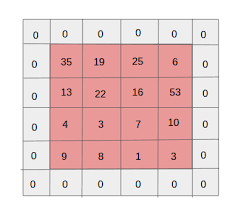
\includegraphics[resolution=100]{Padding.png}
		\caption{Wartości zerowe na krawędziach macierzy tworzą margines.}
\end{figure}

%Pooling
Operacja łączenia to nieodłączny element sieci splotowych idący w parze za operacją nałożenia filtra. Filtr z dodaniem marginesu wewnętrznego  powoduje że wielkość mapy cech pozostaje taka sama jak poprzednia warstwa sygnału wejściowego, ale teraz ma dodatkowe warstwy filtru w zależności od liczby zdefiniowanej przez użytkownika. Łączenie zmniejsza wielkość mapy cech i pozwala jeszcze bardziej wyostrzyć cechy z poprzedniej warstwy oraz obniżyć ilość parametrów, a tym samym złożoność obliczeniową sieci. Dodatkowym atutem jest obniżenia ryzyka przeuczenia sieci, ponieważ największe szczegóły obrazu zostają tutaj wyeliminowane. Zostawiane są tylko cechy ogólne dla danego obiektu. Do łączenia używa się operacji $max()$. Filtr tej warstwy o niewielkim rozmiarze $2x2$ i przesunięciu o $2$, wybiera maksymalną wartość z czterech pól, które są aktualnie przeglądane. W ten sposób następuje redukcja wysokości i szerokości mapy cech, głębokość (ilość filtrów) pozostaje  bez zmian. Przesunięcie i rozmiar filtra są hiperparametrami, zadanie odpowiedniego dobrania ich wartości należy do zadań użytkownika sieci. Zwyczajowo nie używa się zerowych marginesów dla warstw łączących. Warstwa łącząca będzie rozmiarów:

$$ W = \frac{W_1 - F}{P} + 1 $$
$$ S = \frac{S_1 - F}{P} + 1 $$
$$ G = G_1 $$

Gdzie:
\begin{itemize}
\item $W$ -- wysokość
\item $W_1$ -- wysokość poprzedniej warstwy
\item $S$ -- szerokość
\item $S_1$ -- szerokość poprzedniej warstwy
\item $F$ -- rozmiar przestrzeni filtra
\item $P$ -- przesunięcie
\item $G$ -- głębokość
\item $G_1$ -- głębokość poprzedniej warstwy
\end{itemize}

\begin{figure}[ht]
	\centering
			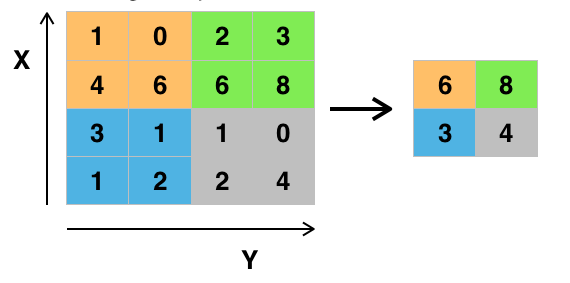
\includegraphics[resolution=100, scale=0.6]{MaxPooling.png}
		\caption{Operacja łączenia MaxPooling.}
\end{figure}

%Współdzielenie parametrów Parameter sharing
\subsection{Współdzielenie parametrów}
Wartości wag są współdzielone między zestaw neuronów podpiętych do wybranego jądra. Jest to technika, która umożliwia istnienie sieci konwolucyjnych. Bez tego głębokie sieci neuronowe byłyby zbyt przeładowane parametrami by podołać złożoności obliczeniowej. Założenie współdzielenia parametrów miedzy neuronami wynika z założenia, że jeśli dana cecha, np. krawędź, występuje w jednej części obrazu, prawdopodobnie będzie się powtarzać w również innych fragmentach. Można wykorzystać zjawisko powtarzalności wzorców i używać raz zdefiniowaną cechę, na całym obrazie zamiast definiować ją na nowo dla każdego fragmentu obrazu.

Współdzielone wagi filtru oznaczają że jeden filtr jest stały dla całej powierzchni obrazu wejściowego, przesunięcie filtra po całym obrazie nie zmienia jego wag, dzieje się to dopiero podczas aktualizacji wag w trakcie wykonania wstecznej propagacji błędu. Powtarzalne cechy są znajdowane niezależnie od tego, który region obrazu wejściowego jest rozpatrywany.

Dla przykładu obraz o rozmiarach 3x3, mając nałożony filtr o rozmiarach 2x2 otrzyma do przeliczenia operacje:

 $$X = 
 \begin{bmatrix} 
 x_{11} & x_{12} & x_{13}  \\ x_{21} & x_{22} & x_{23} \\x_{31} & x_{32} & x_{33} 
 \end{bmatrix}
$$
$$F =  
 \begin{bmatrix} 
 w_{11} & w_{12} \\ w_{21} & w_{22} 
 \end{bmatrix}
$$
 $$\beta = 
 \begin{bmatrix} 
 w_{11}, & w_{12}, & w_{21}, & w_{22} 
 \end{bmatrix}
$$
 $$F * X =  
 \begin{bmatrix}  
\beta \cdot [x_{11}, x_{12}, x_{21}, x_{22}] & \beta \cdot [x_{12}, x_{13}, x_{22}, x_{23}] \\
\beta \cdot [x_{21}, x_{22}, x_{31}, x_{32}] & \beta \cdot [x_{22}, x_{23}, x_{32}, x_{33}] 
 \end{bmatrix}
$$

\subsection{Warstwy gęste}
Warstwa w której wszystkie neurony są połączone ze wszystkimi neuronami kolejnej warstwy nazywa się w pełni połączoną (ang. fully connected layer) oraz wartwą gęstą (ang. dense layer). Jest to typ warstwy używany w tradycyjnych sieciach neuronowych gdzie naturalnymi są połączenia każdy z każdym. W splotowej sieci neuronowej jest to ostatni niezbędny budulec zaraz za warstwami konwolucji i warstwami łączącymi.

Warstwy gęste stosuje się na końcu architektury sieci, gdzie neurony już głosują jaka jest poprawna odpowiedź. Podczas trenowania sieci, korekcja wag sprawia że wybór klasy wyjściowej ma się odbyć na podstawie cech znalezionych w poprzednich warstwach. Kiedy już sieć jest wyuczona i otrzyma przykład do sklasyfikowania, następuje głosowanie przez wszystkie neurony, algorytm liczy średnie prawdopodobieństwo dla każdej wybranej przez każdy neuron klasy wyjściowej i wybiera jako odpowiedź o największym prawdopodobieństwie (największej średniej sumie wag). W ten sposób lista cech z poprzednich warstw staje się listą ''głosów''.

\subsection{Rekurencyjne sieci neuronowe}
Sieci które zawierają sprzężenia zwrotne, czyli połączenia które zwracają sygnał z neuronów do wcześniejszych warstw sieci. Ta charakterystyka daje sieci nowe możliwości. Sieć ze sprzężeniem zwrotnym generuje zjawiska niedostępne w sieciach jednokierunkowych. Sieć jednym wejściem może wygenerować sekwencję sygnałów, ponieważ sygnały z wyjścia jednego kroku, wracając na wejście neuronów warstw wcześniejszych generują nowe, zupełnie inne wartości. Kilka ciekawych zjawisk opisywanych w sieciach rekurencyjnych to nagły wzrost i osłabienie wag sygnałów, chaotyczne błądzenie wartości po sieci. Wymienione charakterystyki są ciekawe, ale powodują mała popularność sieci rekurencyjnych przez trudność analizy zachowań i złożoność obliczeniową. Na chwilę obecną, stosowane są głównie w miejscach mających dostęp do ogromnych centrów obliczeniowych, przykładami są, asystentka Siri w urządzeniach firmy Apple oraz Google Translator. W zastosowaniach medycznych, obiecujące są zastosowania do analizy składania białek i analiza sekwencji DNA.

\begin{figure}[ht]
	\centering
			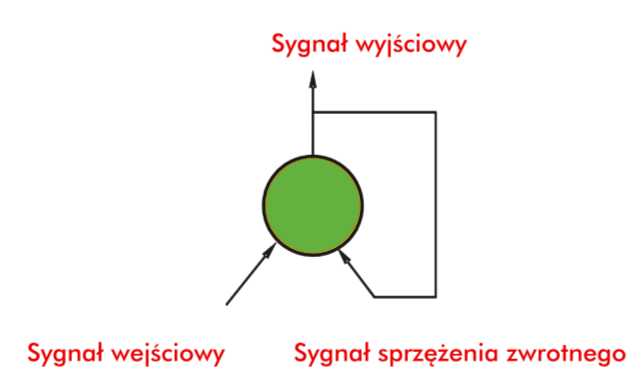
\includegraphics[resolution=100, scale=0.5]{recurrentNeuralNetwork.png}
		\caption{Pojedynczy neuron ze sprzężeniem zwrotnym.}
\end{figure}

Dla poprawnego zakończenia przejścia przez sieć, sygnał musi osiągnąć stan równowagi. Stan równowagi osiąga się przez mnożenie iloczynu sygnału wejściowego z wagą wejścia. Wynik powinien być równy sygnałowi sprzężenia zwrotnego dający wartość do wytworzenia tego sygnału wejściowego.

Obiecującą charakterystyką rekurencyjnych sieci neuronowych jest posiadanie wewnętrznej pamięci. Daje to możliwość zapamiętania informacji o sygnałach wejściowych, w wielu architekturach używa się pamięci do przewidywania co jaki będzie następny sygnał. Obecnie częstotliwość zastosowań tego typu sieci może wzrosnąć jeśli zostaną zaimplementowane z uwzględnieniem problemów wydajnościowych, tzn. ograniczenie głębokości sieci i skrócenie ilości przejść sygnału przez sieć. Testując prymitywną sieć rekurencyjną pierwszym zaskoczeniem staje się ilość przejść sygnału zanim wartości osiągną stan równowagi.

Wielu badaczy \cite{siteRNN} przewiduje,  że po rozwiązaniu problemów wydajnościowych sprzężenie zwrotne okaże się preferowanym sposobem na uczenie neuronów. W szczególności świetnie sprawdzają się dla danych sekwencyjnych, takich jak mowa, text, audio oraz obrazy. Posiadają to czego brakuje w wielu innych sieciach, kontekst. Do standardowej rekurencyjnej sieci neuronowej posiadającej tylko pamięć krótkotrwałą, można dołączyć wynaleziony w 1997 roku, mechanizm LSTM (ang. Long-Short Term Memory). 

Mająca dwa sygnały wejściowe sieć rekurencyjna stosuje liczenie wag na obu wejściach. Wagi są korygowane algorytmem gradientu spadkowego oraz wstecznej propagacji błędu w czasie (ang. Backpropagation Through Time). Istotną obserwacją jest możliwość mapowania jednego wejścia na wiele wyjść, wielu wejść do wielu wyjść oraz wiele wejść do jednego wyjścia, w dowolnej kombinacji ilości. Wsteczna propagacja błędu w czasie działa jak zwykła propagacja, z drobną różnicą, że sieć jest rozwijana. Korekta wag następuje od końca przez wszystkie cykle w których wystąpiła rekurencja, to znaczy jeśli sygnał przechodził przez ten sam neuron $t$ razy, wtedy następuje rozwinięcie sekwencji dla $t$ operacji i algorytm wykonuje korekcje jakby były to osobne sieci neuronowe zależne od siebie. Tutaj pojawia się wspomniana wcześniej złożoność obliczeniowa.

\begin{figure}[ht]
	\centering
			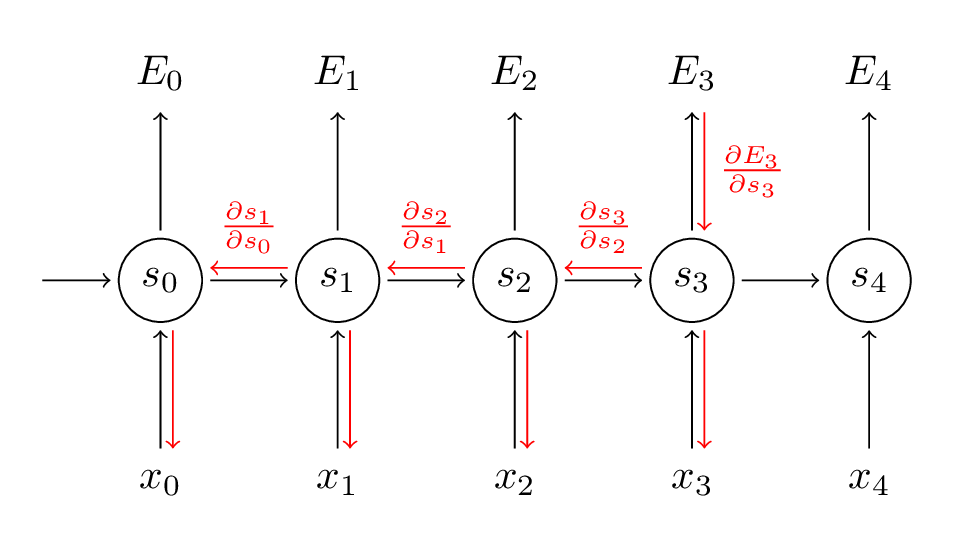
\includegraphics[resolution=100, scale=0.55]{backpropagationThroughTime.png}
		\caption{Wsteczna propagacja błędu w czasie. x - sygnał wejściowy, s - funkcja aktywacji, E - funkcja błędu}
\end{figure}

\subsection{W pełni konwolucyjna sieć neuronowa}

\begin{figure}[ht]
	\centering
			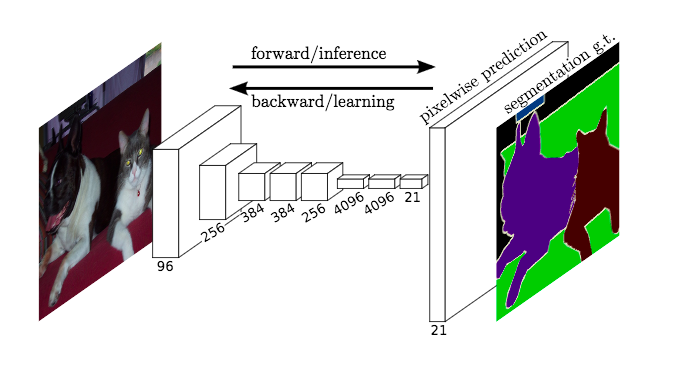
\includegraphics[resolution=100, scale=0.8]{fullyConvolutionalNetwork.png}
		\caption{Wizualizacja architektury FCN przeznaczonej do segmentacji obrazu.}
\end{figure}
W budowie sieć ta przypomina normalną konwolucyjną sieć neuronową, w której ostatnia warstwa jest zastąpiona warstwą konwolucyjną z dużym polem recepcyjnym. Warstwa ta ma pomóc określić kontekst całego obrazu, np. sytuację na drodze w systemie autopilota gdzie istotne jest położenie konkretnych elementów na drodze. Bardzo ważnym jest dobranie odpowiednio dużej ostatniej warstwy konwolucyjnej, pozwoli to na dokładne określenie rozmieszczenia wykrytych obiektów. Ta warstwa jest używana jako klasyfikator każdego piksela na obrazie.

Docelowo wynik takiej sieci jest obrazem o identycznym rozmiarze co sygnał wejściowy. Obraz przypomina sygnał wejściowy w dużym uproszczeniu gdzie wykryte obiekty są zamalowane jednolicie każdy segment innym kolorem.

Zamiana zwykłej CNN na FCN (ang. Fully Convolutional Network) może być stosowana dla dowolnej architektury, mając przewagę nad innymi, ponieważ wykorzystanie gotowych architektur znacząco skraca czas na tworzenie działających aplikacji. Mając wytrenowaną sieć konwolucyjną, należy podmienić wszystkie w pełni połączone warstwy (ang. fully connected) na warstwy konwolucyjne. Ostatnią warstwę wyjściową docelowo należy ustalić na rozmiar identyczny z warstwą wejściową z ilością kanałów odpowiadającą ilości klas.

Jak wiadomo sieci splotowe zmniejszają przestrzenie obrazów na kolejnych warstwach, więc by uzyskać znów pierwotny rozmiar obrazu na wyjściu sieci, należy skorzystać z mechanizmu konwolucji wstecznej. Jest to ta sama operacja co konwolucja, operacje są wykonywane w odwróconej kolejności, a wagi korygowane są identycznie.\cite{DBLP:journals/corr/LongSD14}

\subsection{Pozostałe typy sieci neuronowych}
Opisanie topologii pozostałych typów sieci neuronowych jest zadaniem wykraczającym za niniejszą pracę. Poniżej znajduje się lista najczęściej stosowanych topologii. Lista została opublikowana w 2016 roku przez Fjodor van Veen wraz z opisem każdego elementu.\cite{siteFjodorList}

\begin{itemize}
\item Radial basis network,
\item Long / Short Term Memory,
\item Gated Recurrent Unit,
\item Auto Encoder,
\item Variational Auto Encoder,
\item Denoising Auto Encoder,
\item Sparse Auto Encoder,
\item Markov Chain,
\item Hopfield Network,
\item Boltzman Machine,
\item Restricted Boltzman Machine,
\item Deep Belief Network,
\item Deconvolutional Network,
\item Deep Convolutional Inverse Graphics Network,
\item Generative Adversarial Network,
\item Liquid State Machine,
\item Extreme Learning Machine,
\item Echo State Network,
\item Deep Resisdual Network,
\item Kohonen Network,
\item Support Vector Machine,
\item Neural Turing Machine.
\end{itemize}

% ################################
%        BIBLIOTEKI
% ################################
\chapter{Biblioteki implementujące uczenie głębokich sieci neuronowych}
Nagły wzrost zainteresowania sieciami neuronowymi, spowodował pojawienie się wielu bibliotek implementujących algorytmy do pracy z głębokimi sieciami neuronowymi, a także przy okazji wiele pobocznych zadań Machine Learningu. Obecnie wiele z największych firm technologicznych próbuje wypromować własny stos technologiczny oparty o licencje zapewniające każdemu dostęp do źródeł. Otwartość nie wynika z dobroduszności i chęci dzielenia się ze społecznością, a wspólnym mianownikiem wszystkich narzędzi jest kompletne API dla użytkowników języka Python. Jest to język w którym najszybciej można znaleźć literaturę wprowadzającą w zagadnienie. \cite{siteDLByLanguage}

Na uwagę zasługuje fakt pojawienie się kilku bibliotek napisanych wyłącznie dla JavaScript'u. Ich zastosowanie jest nastawione na użytkowników gotowych modeli i ogranicza się głównie do importu zminiaturyzowanych wag na telefon by szybko odpowiadać na sygnały użytkownika takie jak zdjęcie z aparatu, bądź komendę głosową. 

\subsection{Tensorflow}
\begin{figure}[ht]
	\centering
			
\includegraphics[resolution=100, scale=0.6]{Tensorflow.png}
		\caption{Logo biblioteki Tensorflow}
\end{figure}

Tensorflow jest pierwszą otwartoźródłową biblioteką dla obliczeń numerycznych używająca grafów przepływu danych. Umożliwia praktykom uczenia maszynowego wykonywać intensywne obliczenia na danych przez wydajną implementację powszechnie używanych algorytmów głębokiego uczenia. Węzły w grafie przepływu są reprezentowane jako operacje matematyczne, zaś wierzchołki przedstawiają wielowymiarowe macierze (tensory) zapewniające komunikacje między wierzchołkami i węzłami. Architektura tworzonych sieci w Tensorflow jest łatwa w modyfikacji, dlatego jeden model można wykorzystać do pracy z procesorami CPU, GPU, urządzeniami mobilnymi i chmurą mieszaną. \cite{DeepLearningTensorflow}

Pierwotnie Tensorflow umożliwiał pracę tylko z językiem Python. Od wersji 1.0 dodano eksperymentalne API do Javy i Golang. Ta wersja zadebiutowała z innowacyjnym narzędziem Tensorflow Debugger. Jest on narzędziem tekstowym do debugowania działających aplikacji.

Należy zaznaczyć że biblioteka jest wieloplatformowa i działa na wszystkich popularnych systemach operacyjnych:
\begin{itemize}
\item Windows
\item Linux
\item Mac
\item Android
\item iOS
\item Raspberry PI
\end{itemize}

Zestaw narzędzie zawiera \textit{Tensorflow Board} graficzne oprogramowanie do analizy utworzonych modeli. Łatwość użycia i przyjęcie modelu Open Source sprawia że jest to najczęściej używana biblioteka podczas prac naukowych, o czym świadczy ilość cytowań. \cite{siteTensorflowCitations} Wiele firm wspiera projekt używając kodu i dodając do niego własne rozszerzenia, warto wymienić choćby kilku większych kontrybutorów:
\begin{itemize}
\item Google,
\item ARM,
\item Twitter,
\item Ebay,
\item Intel,
\item Qualcomm
\end{itemize}

Główne zalety:
\begin{itemize}
\item Największe zasoby dokumentacji i kursów w sieci,
\item Oglądanie w czasie rzeczywistym procesu uczenia przez \textit{Tensorboard},
\item Największa społeczność programistów skupiona wokół projektu spośród wszystkich bibliotek,
\item Wspiera uczenie rozproszone na wielu maszynach,
\item Biblioteki pokrewne, korzystające ze wspólnego silnika \textit{Tensorflow Lite} i \textit{Tensorflow.JS} umożliwiają zastosowanie tych samych modeli na urządzeniach mobilnych i przeglądarkach.
\end{itemize}

Tensorflow ma dwie wady, działające na niekorzyść osób zaczynających pracę z sieciami neuronowymi:
\begin{itemize}
\item Wymaga sporej ilości kodu do utworzenia działającego modelu, przez co uważany jest za bibliotekę niskopoziomową w porównaniu do pozostałych,
\item Kompletne wsparcie istnieje tylko dla języka Python, 
\item Jest dużo wolniejszy od CNTK i MXNet \cite{DBLP:journals/corr/ShiWXC16}
\end{itemize}

\noindent
\newline 
Dokumentacja: https://www.tensorflow.org/api\_docs/python/
\newline 
Kod źródłowy: https://github.com/tensorflow
\newline 
Licencja: Apache 2.0

\subsection{Keras}

\lstinputlisting[language=Python]{Keras.py}
\noindent
\begin{minipage}{\linewidth}
\begin{lstlisting}[caption=Skrypt najprostszego modelu sekwencyjnego (Keras w 30 sekund), label=lst:test]
from keras.models import Sequential
from keras.layers import Dense
model = Sequential()
model.add(Dense(units=64, activation='relu', input_dim=100))
model.add(Dense(units=10, activation='softmax'))
model.compile(loss='categorical_crossentropy',
              optimizer='sgd',
              metrics=['accuracy'])
model.compile(loss=keras.losses.categorical_crossentropy,
              optimizer=keras.optimizers.SGD(lr=0.01, momentum=0.9, nesterov=True))
model.fit(x_train, y_train, epochs=5, batch_size=32)
model.train_on_batch(x_batch, y_batch)
loss_and_metrics = model.evaluate(x_test, y_test, batch_size=128)
classes = model.predict(x_test, batch_size=128)
\end{lstlisting}
\end{minipage}

\begin{figure}[ht]
	\centering
			
\includegraphics[resolution=100, scale=0.3]{Keras.png}
		\caption{Logo biblioteki Keras}
\end{figure}

Keras jest frameworkiem udostępniającym wysokopoziomowe API dla głębokich sieci neuronowych. Jego źródła zostały otwarte w 2015 roku. Społeczność skupiona wokół projektu wyróżnia się bardzo pozytywnym podejściem dla osób z poza środowiska naukowego i jest otwarta na propozycje rozwoju biblioteki. Nazwa Keras pochodzi od greckiego słowa \(\kappa\epsilon\rho\alpha\zeta\) oznaczającego róg, geneza nazwy wywodzi się z greckiego eposu Homera pod tytułem Odyseja.

Założeniem François Chollet'a, czyli autora jest zwiększenie szybkości przeprowadzania eksperymentów, dlatego Keras ma wysokopoziomowe API udostępniające uruchomienie algorytmów głębokiego uczenia w kilku liniach kodu. Zalety wymieniane przez autora:
\begin{itemize}
\item Wspieranie łatwego i szybkiego prototypowania (przez modularność, przyjazny interfejs, możliwości rozszerzenia),
\item Wspiera konwolucyjne sieci neuronowe, rekurencyjne sieci neuronowe i umożliwia mieszanie obu,
\item Działa na CPU i GPU.
\end{itemize}

Działanie opiera się na wykorzystaniu rdzenia Tensorflow, CNTK lub Theano jako bibliotek wykonujących obliczenia. Potwierdza to idee stworzenia narzędzia dla szybkiego prototypowania modeli. \cite{bookDeepLearningKeras}

Do zalet można zaliczyć:
\begin{itemize}
\item Najszybsze prototypowanie ze wszystkich rozwiązań na rynku,
\item Uproszczony interfejs zachęca do eksperymentów osoby nie związane z analizą danych,
\item Wbudowane wsparcie do pracy na GPU,
\item Wspiera strumieniowanie danych przez Spark,
\item Działa nie tylko na kartach NVIDIA, ale też Google TPU, AMD
\end{itemize}

Przy dłuższej pracy i bardziej skomplikowanych modelach, wysokopoziomowość interfejsu programistycznego biblioteki ogranicza elastyczność w działaniu. Brak wielu możliwości kontroli sieci, powoduje że poleca się ją głównie dla nowicjuszy oraz eksperymentów przy standardowych typach sieci (konwolucyjnych, rekurencyjnych).

\noindent
\newline 
Dokumentacja: https://keras.io/
\newline 
Kod źródłowy: https://github.com/keras-team/keras
\newline 
Licencja: MIT

\subsection{PyTorch}
\begin{figure}[ht]
	\centering
			
\includegraphics[resolution=100, scale=0.5]{PyTorch.png}
		\caption{Logo biblioteki PyTorch}
\end{figure}

Oprogramowanie wywodzące się ze starej biblioteki \textit{Torch}. Otwartoźródłowy zestaw bibliotek uczenia maszynowego dla języka Python. Stał się zestawem różnych narzędzi od kiedy do głównego repozytorium zaczęto dodawać inne mniejsze biblioteki oraz narzędzia takie jak serwowanie modeli wzdłuż wszystkich platform. Główna biblioteka używana w Facebook'u do przetwarzania języka naturalnego. 

PyTorch dostarcza dwie wysokopoziomowe funkcjonalności:
\begin{itemize}
\item Obliczenia na tensorach z akceleracją obliczeń na GPU,
\item Głębokie sieci neuronowe zbudowane na automatycznie różniczkowalnym systemie taśmowym
\end{itemize}

Główne zalety:
\begin{itemize}
\item Proces modelowania jest prosty i przejrzysty dzięki architekturze opartej na programowaniu imperatywnym,
\item Dynamiczne generowanie grafu sieci,
\item Deklaratywna równoległość danych, czyli dzielenie sygnałów wejściowych na wiele mniejszych,
\item Najbardziej ''pythoniczna'' składnia,
\item Zawiera sporą ilość gotowych do użycia modeli i architektur, pozwalając na kombinację ich w nowe struktury,
\item Graf obliczeniowy jest generowany w trakcie działania programu, co pozwala na używanie dowolnego debuggera i nawet drukowanie obecnego stanu obliczeń na ekran, jest to spory potencjał na narzędzia interaktywne,
\item Służy także jako alternatywa dla NumPy z możliwością obliczeń na GPU,
\item Specjalnie napisane zarządzanie pamięcią GPU, pozwalające na niesamowicie wydajne zarządzanie pamięcią w porównaniu do konkurencji.
\end{itemize}

PyTorch jest jednym z najmłodszych narzędzi, dlatego ma kilka nierozwiązanych jeszcze problemów:
\begin{itemize}
\item Nie jest zalecany do zastosowań produkcyjnych. Obecna wersja jest numerowana 0.4, wersja 1.0 była zapowiedziana na lato 2018. Na wrzesień 2018 brak informacji kiedy nastąpi premiera,
\item Brak gotowych narzędzi do monitoringu i wizualizacji procesu uczenia i podglądu grafu sieci
\end{itemize}\cite{book:2226069}

Język \textit{Pyro} do programowania probalistycznego stworzony przez firmę Uber opiera się na PyTorch.

\noindent
\newline
Dokumentacja: https://pytorch.org/docs/stable/index.html
\newline
Kod źródłowy: https://github.com/pytorch/pytorch
\newline
Licencja: Brak określonej. Prawa autorów zastrzeżone, oprogramowanie ''as is''.


\subsection{Tensorflow.js [Deeplearn.js]}
\begin{figure}[ht]
	\centering
			
\includegraphics[resolution=100, scale=0.6]{TensorflowJS.png}
		\caption{Logo biblioteki Tensorflow.js}
\end{figure}

W 2017 roku został opublikowany projekt o nazwie Deeplearn.js z celem wprowadzenia uczenia maszynowego i głębokiego uczenia do przeglądarek internetowych bez konieczności korzystania z zewnętrznego API.

JavaScript kojarzony jest jeszcze często przez programistów nie aktualizujących wiedzy z programowania front-end'u jako powolny interpretowany język ograniczony do pracy w obrębie jednego procesu procesora CPU. \cite{siteSlowJavaScript} Aby uniknąć restrykcji wydajnościowych zaimplementowano wykonanie operacji na WebGL, interfejsowi OpenGL działającym na przeglądarkach internetowych.

W maju 2018 zespół odpowiedzialny za rozwój DeepLearn.js został połączony z zespołem programistów pracujących przy Tensorflow, a biblioteka zmieniła nazwę na Tensorflow.js. Dostarcza calej mocy Tensorflow do przeglądarki czy dowolnego interpretera kodu Javascript jak Node.js.

Tensorflow.js nie ma wspólnej bazy kodu z Tensorflow, również filozofia działania jest inna. Należy podkreślić że zbieżność nazw wynika z połaczenia pracy dwóch zespołów w jedną jednostkę. Interfejs programistyczny udostępniany przez framework javascriptowy udostępnia zarówno niskopoziomowe elementy do uczenia maszynowego oraz wysokopoziomy interfejs wzorowany na tym z biblioteki Keras do tworzenia sieci neuronowych.

Biblioteka na podstawowym poziomie dostarcza dwa elementy:
\begin{itemize}
\item CoreAPI -- komponent zarządzający kodem niskopoziomowym,
\item LayerAPI -- komponent zbudowany na CoreAPI, udostępnia abstrakcje wyższego poziomu
\end{itemize}

Podstawową jednostką danych jest tensor, czyli zbiór wartości liczbowych ułożonych w tablicę jedno lub więcej wymiarową. Tensor definiuje się konstruktorem \textit{tf.tensor}, gdzie należy określić tablice oraz kształt tensora. Istnieje wiele metod pozwalających na stworzenie tensorów różnych kształtów takich jak \textit{tf.zeros} do wypełnienia podanego kształtu zerami, oraz takie jak \textit{tensor1d, tensor2d, tensor3d, tensor4d} dla ułatwienia czytelności przy tworzeniu najczęściej używanych rozmiarów.
Tensory są niezmienne co oznacza że raz stworzony tensor nie może zmieniać wartości. 

Zmienne (ang. variables) są inicjalizowane wartościami tensorów co daje możliwość modyfikowania ich wartości, używa się ich do trzymania i aktualizacji wartości w trakcie trenowania modelu.

Operacje (ang. operations [Ops]) to metody pozwalające na modyfikacje danych. \textit{Tensorflow.js} udostępnia całą gamę operacji do pracy z machine learningiem. Działają one na tensorach przez zwracanie wyniku operacji jako nowy tensor.

Powyższe struktury danych należą do CoreAPI, druga warstwa operacji LayerAPI operuje na wyższym poziomie abstrakcji i zapewnia zupełnie inne bloki do budowy sieci neuronowych. Najważniejsze atuty tej warstwy to wysokie podobieństwo do kodu tworzonego w Keras, możliwość naśladowania stylu programowania znanego z języka Python. Poniżej prezentowany jest kod porównawczy między pythonową wersją tego samego kodu i javascriptową reprezentacją z użyciem \textit{Tensorflow.js}. Kod wykonujący intensywne operacje napisany jest asynchronicznie. Największą zaletą może się jednak okazać brak konieczności używania NumPy, którego w JavaScript brakuje. Wszystkie operacje matematyczne wymagane do uczenia maszynowego z NumPy zostały zaimplementowane w bibliotece. \cite{siteTensorflowJSConcepts}

\noindent
\begin{minipage}{\linewidth}
\begin{lstlisting}[caption=Proste operacje w JavaScript z Tensorflow.js, label=lst:test]
import * as tf from '@tensorlowjs/tfjs';
const model = tf.sequential();
model.add(tf.layers.dense({units: 1, inputShape: [1]}));
model.compile({optimizer: 'sgd', loss: 'meanSquaredError'});
const xs = tf.tensor2d([[1], [2], [3], [4]], [4, 1]);
const ys = tf.tensor2d([[1], [3], [5], [7]], [4, 1]);
await model.fit(xs, ys, {epochs: 1000});
model.predict(tf.tensor2d([[5]], [1, 1])).print();
\end{lstlisting}
\end{minipage}

\noindent
\begin{minipage}{\linewidth}
\begin{lstlisting}[caption=Prosty model w języku Python używając Keras, label=lst:test]
import keras
import numpy as np
model = keras.Sequential()
model.add(keras.layers.Dense(units=1, input_shape=[1]))
model.compile(optimizer='sgd', loss='mean_squared_error')
xs = np.array([[1], [2], [3], [4]])
ys = np.array([[1], [3], [5], [7]])
model.fit(xs, ys, epochs=1000)
print(model.predict(np.array([[5]])))
\end{lstlisting}
\end{minipage}

\noindent
\newline
Dokumentacja: https://github.com/tensorflow/tfjs
\newline
Kod źródłowy: https://js.tensorflow.org/
\newline
Licencja: Licencja: Apache 2.0

\subsection{PaddlePaddle}
\begin{figure}[ht]
	\centering
			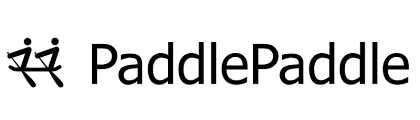
\includegraphics[resolution=100, scale=1.2]{PaddlePaddle.png}
		\caption{Logo biblioteki Paddle}
\end{figure}
Pełna nazwa biblioteki ''\textbf{PA}rallel \textbf{D}istributed \textbf{D}eep \textbf{LE}arning''. Oprogramowanie skierowane głównie na jeden rynek, mało znane w Europie / USA. Jest to zaś najpopularniejszy framework w Chinach. Tworzony i utrzymywany przez firmę Baidu, znaną jako chiński klon Google. Założona w 2000 roku przeniosła pomysł na wyszukiwarkę internetową na chiński rynek i od tej pory z powodzeniem kopiuje wszystkie technologie i pomysły Google, w tym autonomiczne samochody. 

Problemem jaki może napotkać osoba nie znająca języka chińskiego jest częste zgłaszanie uwag i komentarzy do kodu bez opisu w języku angielskim. Kursy praktycznego wykorzystania narzędzia udostępniane w internecie pochodzą głównie od pracowników firmy Baidu, a kierowane są najczęściej dla studentów chińskich uniwersytetów, stąd bardzo mała popularność poza rodzimym rynkiem. Ze strony domowej można wyczytać często powtarzające się słowa o ''prostocie użycia'', ''prostocie działania''. 

Przechodząc do treści technicznych, PaddlePaddle opisywany jest jako zestaw narzędzi i bibliotek do uczenia głębokiego bazujący na ''języku programowania do uczenia głębokich sieci neuronowych''. Biblioteka jest bardzo elastyczna i pozwala na tworzenie dowolnego kształtu modeli. Jak w Tensorflow tak i tutaj istnieje graficzne narzędzie wizualizacji nauczania \textit{Visual Deep Learning}, narzędzie pozwala wyświetlić wydajność trenowania i statystyki danych takie jak dokładność, wartości funkcji kosztu, rozkład parametrów, próbki obrazu i dźwięku, wykres ONNX modelu.

Na podstawie biblioteki istnieje cała społeczność i inicjatywa \textit{EasyDeepLearning}, mająca ułatwić firmom nie zatrudniającym specjalistów od algorytmów uczenia maszynowego na wykonanie szybkich i sprawnych modeli bez konieczności posiadania terabajtów danych. Społeczność skupia się głównie w ośrodkach akademickich i start-upach w Chinach, gdzie PaddlePaddle jest standardem.

Same możliwości biblioteki są potężne, pozwala na budowę:
\begin{itemize}
\item Botów dzięki technologii Word2Vec,
\item Systemów rekomendacji,
\item Klasyfikatorów obrazów,
\item Translacji maszynowej języków z użyciem głębokiego uczenia,
\item Detekcji obiektów na obrazie filmów z użyciem Single Shot Multibox Detector,
\item Analizatora nastrojów
\end{itemize}

Przy bliższym spotkaniu, widać że jest to klon Tensorflow, który ze względu na brak konkurencji w Chinach jest dużo szybciej rozwijany, a jego możliwości w zakresie uczenia na farmach serwerów przewyższają pierwowzór. Z produktów opartych na Baidu korzysta prawie miliard osób, stąd bardzo duży nacisk na optymalizację i własne rozwiązania technologiczne przekładają się na wysoką wydajność.

\noindent
\newline
Dokumentacja: http://www.paddlepaddle.org/documentation/en
\newline
Kod źródłowy: https://github.com/PaddlePaddle/Paddle
\newline
Licencja: Apache 2.0

\subsection{MXNet}
\begin{figure}[h]
	\centering
			
\includegraphics[resolution=100,scale=2]{MXNet.png}
		\caption{Logo biblioteki MXNet}
\end{figure}

Biblioteka do głębokiego uczenia stworzona przez fundację Apache. Wspiera największą ilość języków ze wszystkich dostępnych bibliotek:
\begin{itemize}
\item Python,
\item C++,
\item Cloujure,
\item Julia,
\item Perl,
\item R,
\item Scala
\end{itemize}

O popularności i powszechne przyjęciu świadczy implementacja na chmurach Microsoft Azure, Intel i Amazon Web Services. Główne zastosowania do których MXNet jest używany to rozpoznawanie mowy i pisma ręcznego, przetwarzanie języka naturalnego i przewidywanie zdarzeń. Użycie skupia się w kręgach przedsiębiorstw, trudno zatem znaleźć badania akademickie przeprowadzane z wykorzystaniem tej biblioteki.

Kolejnym atutem MXNet jest przenośność modeli. Są one zoptymalizowane by nie zajmować dużo pamięci, pozwala to na przeniesienie modelu wytrenowanego w chmurze do urządzenia mobilnego jak smartfon. Łatwe serwowanie modeli, skalowanie na żądanie z mieszaniem GPU i CPU jest zdecydowanie największymi atutami dlaczego Amazon wybrał tą bibliotekę jako pierwszą na swoje centra obliczeniowe. \cite{book:2256184}

Gluon jest API wysokiego poziomu dostarczanym wraz z MXNet. Jego zadaniem jest dostarczyć czystej, spójnej i prostej składni bez obniżania wydajności działania aplikacji. Istnieje również druga warstwa API wysokopoziomowego (można wybierać, z której chce się korzystać) o nazwie Module. Ta warstwa skupia się na pracy z Symbol, paczką do przetwarzania wyrażeń symbolicznych. \cite{DBLP:journals/corr/ChenLLLWWXXZZ15} Jego najlepszymi atutami są:
\begin{itemize}
\item uproszczenie składni budowanych sieci neuronowych, przypominają one pseudokod,
\item elastyczna struktura zapewniająca kod imperatywny,
\item dynamiczny graf sieci, umożliwia zmiany struktury sieci w trakcie działania programu,
\item ładowanie sieci neuronowej do pamięci podręcznej poprawia wydajność, w tym celu używa się modelu sieci \textit{HybridSequential}
\end{itemize}

\noindent 
\newline
Dokumentacja: https://mxnet.apache.org/api/
\newline
Kod źródłowy: https://github.com/apache/incubator-mxnet
\newline
Licencja: Apache 2.0

\subsection{Caffe2}
\begin{figure}[h]
	\centering
			
\includegraphics[resolution=100, scale=0.35]{Caffe2.png}
		\caption{Logo biblioteki Caffe2}
\end{figure}

Biblioteka wywodzi się z architektury Caffe, narzędzia dla praktyków głębokich sieci neuronowych udostępniającego przejrzystą składnię API w czasach przed pojawieniem się bibliotek wspieranych przez wielkie korporacje. Pierwsza wersja napisana przez Yangqing Jia w trakcie doktoratu na uniwersytecie Berkeley, obecnie jest dyrektorem działu AI w Facebook'u, gdzie rozwijany jest Caffe2. \cite{jia2014caffe} O wieku świadczy dobór języków dostępnych do wykorzystania w bibliotece:
\begin{itemize}
\item C++
\item Python
\item MATLAB
\end{itemize}

Caffe2 jest rozwinięciem tego modelu, również pracuje na GPU, CPU, jest skalowalny, posiada spore wsparcie społeczności. Różnica jest w modyfikacji architektury obliczeniowej. Główną przewagą jest prosta skalowalność na wiele maszyn i urządzenia mobilne. Taki podział na komponenty i elastyczność w wykorzystaniu podzespołów nazywana jest odframeworkowaniem (ang. un-framework) poprzedniej wersji.
\cite{DBLP:journals/corr/JiaSDKLGGD14}

Cała baza została napisana w języku C++ i była testowana latami przez Facebook'a do rozpoznawania obiektów na obrazie, analizy wiadomości do rekomendowania reklam, systemów rekomendujących na podstawie profilu użytkownika. Wydajność jest to jedną z największych zalet, po opracowaniu odpowiedniej architektury, cały kod wdrożeniowy na produkcję może być napisany w C++. Na jednym procesorze NVIDIA DGX-1 prędkość przetwarzania wynosi 231 obrazów na sekundę. \cite{siteNvidiaCaffe2}

Caffe2 posiada zoo modeli, gotowe do użycia wcześniej wyuczone modele dla najczęściej spotykanych zastosowań bez potrzeby wydawania zasobów na tworzenie modelu od zera. Pełna lista modeli, z którymi można eksperymentować jest pokaźna (na dzień obecny największa ze wszystkich dostępnych zwierząt w ZOO):
\begin{itemize}
\item AlexNet,
\item GoogleNet,
\item RCNN ILSVRC13,
\item Densenet 121,
\item Detectron,
\item Inception v1,v2,v3,
\item Resnet 50,
\item SqueezeNet,
\item VGG 19,
\item ZFNET 512
\end{itemize}

Dojrzałość produktu sprawiła że istnieje wiele narzędzi programistycznych ułatwiających pracę z biblioteką. Programiści aplikacji mobilnych mają do dyspozycji wtyczki integracyjne do Visual Studio, Android Studio, Xamarin. Dla pozostałych Caffe2 jest dostępne na każdy popularny system operacyjny oraz u dostawców usług chmurowych. Kod napisany na jedną platformę jest przenaszalny na pozostałe bez konieczności modyfikacji.

Od kwietnia 2018 roku, repozytorium Caffe2 jest przenoszone do katalogu PyTorch. Facebook zdecydował się na zwiększenie kompatybilności przez stopniowe połączenie bazy kodu. Docelowo Caffe2 ma być głównym modułem dla rozwiązań mobilnych, a PyTorch dla całej reszty.

\noindent
\newline
Dokumentacja: https://caffe2.ai/docs/
\newline
Kod źródłowy: https://github.com/caffe2/caffe2
\newline
Licencja: Apache 2.0 (Caffe 1 -- BSD)


\subsection{ML.NET}
\begin{figure}[h]
	\centering
			
\includegraphics[resolution=100, scale=1]{ML_NET.png}
		\caption{Logo biblioteki ML.NET}
\end{figure}
Nowe oprogramowanie od Microsoftu, data wydania pierwszej wersji poglądowej 7 maj 2018. Microsoft tworząc to oprogramowanie wybrał jako grupę docelową programistów skupionych w ekosystemie .NET. API biblioteki udostępnione jest w językach C++ oraz C\#, przy czym kompletna dokumentacja jest tylko dla języka C\#. Docelowo ma stać się częścią .NET Core. Oprogramowanie od początku istnienia powstaje jako otwartoźródłowe, a Microsoft przy każdym wydaniu zachęca do zgłaszania uwag oraz propozycji dalszego rozwoju lub nowych funkcjonalności. Jest to odejście od tradycyjnego modelu utrzymywania oprogramowania w tajemnicy do czasu premiery. Nastawienie na łatwość integracji z oprogramowaniem biznesowym, chmurą Azure oraz łatwość obsługi przez programistów pracujących w technologiach Microsoftu ma zachęcić do wykorzystania oprogramowania na szerszą skalę kiedy wyjdzie ono z fazy rozwojowej i zastąpi CNTK.

W odróżnieniu od pozostałych na chwilę obecną ML.NET jest biblioteką głównie przeznaczoną do uczenia maszynowego, wyewoluowaną z wewnętrznych rozwiązań Microsoftu od lat używanych w zespołach Windows, Bing, Azure. Microsoft przyznaje że jest to przepisywanie większego systemu do świata otwartego oprogramowania. \cite{siteMLNet} Możliwości biblioteki można rozszerzać przez podłączenie modeli z innych bibliotek, wspierane od początku są Tensorflow, Caffe2, CNTK oraz Accord.NET. Sporym atutem jest natywne wsparcie w Azure każdej nowej wersji natychmiast po premierze. Wersja 0.3 przyniosła wsparcie dla formatu modeli ONNX. Narzędzia do głębokiego uczenia pojawiły się w wersji 0.5, zaprezentowanej 12 września 2018. Integracja modeli z Tensorflow umożliwia przeniesienie środowiska z testowego do modelu E2E (ang. Enterprise-2-Enterprise) ''Przedsiębiorstwo-do-przedsiębiorstwa''. Jest to jeszcze zbyt niedojrzała biblioteka by opisywać jej architekturę, nie jest nawet zalecana do rozwiązań produkcyjnych, programiści .NET prawdopodobnie będą z niej chętniej korzystali po pojawieniu się pierwszej kompletnej wersji, co ma nastąpić do wydarzenia \textit{BUILD 2019}. Obecnie traktowana jest jako sposób na przyciągnięcie do ekosystemu .NET Core osób tworzących rozwiązania dla przedsiębiorstw. ML.NET ma jeszcze wiele braków i wad (konieczność programowania skalowania, brak wsparcia platform mobilnych i wyłączność na chmurę Azure), które uniemożliwiają traktowanie go jako poważnego narzędzia komercyjnego w przeciwieństwie do kolejnego narzędzia Microsoftu CNTK.

\noindent
\newline
Dokumentacja: https://docs.microsoft.com/en-us/dotnet/machine-learning/
\newline
Kod źródłowy: https://github.com/dotnet/machinelearning
\newline
Licencja: MIT

\subsection{CNTK}
\begin{figure}[h]
	\centering
			
\includegraphics[resolution=120]{CNTK.png}
		\caption{Logo biblioteki CNTK}
\end{figure}
Nazwa kompletna ''Microsoft Cognitive Toolkit''. Jest to zestaw narzędzi stworzonych w dziale badań i rozwoju Microsoftu, zajmującego się Deep Learningiem. W 2015 zgodnie z nowym modelem biznesowym, nastawionym na częściowe otwieranie kodu źródłowego narzędzi używanych wewnątrz Microsoftu, CNTK został opublikowany na platformie GitHub w kwietniu tego roku. Microsoft wcześniej korzystał z powodzeniem z biblioteki do trenowania modeli usług krytycznych biznesowo. Architektura jest skupiona wokół głębokiego uczenia sieci neuronowych, a dopiero później dodano pozostałe popularne algorytmy uczenia maszynowego.

CNTK posiada zaimplementowane najczęściej używane narzędzia do głębokich sieci neuronowych, takie jak struktury sieci konwolucyjnych czy rekurencyjne sieci neuronowe. Także algorytmy spadku gradientowego i wsteczna propagacja błędów zostały zaimplementowane z automatycznym wykonywaniem równoległych obliczeń z pojedynczego CPU na wiele procesorów GPU na wielu komputerach w sieci. Biblioteka ta jest jednym z backendów do biblioteki Keras, jednak w przeciwieństwie do Keras'a działa tylko na systemach Windows i wybranych dystrybucjach GNU\\Linux.

Niesamowicie wartościowym atutem jest z pewnością dokumentacja dostarczana przez Microsoft. Nie tylko jest ona przejrzysta i spójna z resztą dokumentacji ekosystemu .NET, ale również dostarcza dziesiątek tutoriali krok po kroku jak budować zaawansowane modele, czyścić dane i wyciągać z nich wnioski. Przestawia nawet w jaki sposób przygotowane już rozwiązania przenieść na chmurę Azure i umożliwić korzystanie z nich klientom. Dla osób nie mających podłoża w Data Science, są gotowe przepisy, czyli przygotowane wcześniej szablony do działania na Azure z interfejsem graficznym instruującym jak przygotować dane aby otrzymać gotową usługę. \cite{book:2187021}

\noindent
\newline
Dokumentacja: https://www.microsoft.com/en-us/cognitive-toolkit/
\newline
Kod źródłowy: https://github.com/Microsoft/CNTK
\newline
Licencja: MIT


% ################################
%        ARCHITEKTURA
% ################################

\chapter{Architektura}
\section{Znaczenie architektury dla wydajności sieci}
Elementy sieci neuronowych można ułożyć na nieskończenie wiele sposobów, wystarczy dodać kolejną warstwę neuronów lub zmodyfikować wielkość warstwy i wyniki będą zgoła inne. Celem szukania odpowiedniej dla danego zadania architektury jest otrzymanie najlepszej wydajności klasyfikacji przy skończonym i możliwie jak najkrótszym czasie uczenia. Chcąc uzyskać dobre rezultaty bez eksperymentów od zera, należy wybrać architekturę, która została wykorzystana do rozwiązania podobnego zadania bądź przetestować kilka gotowych architektur z wyuczonymi modelami, a następnie sprawdzić jak się zachowują dla posiadanych zbiorów danych na różnych hiperparametrach.

Architektury ze względu na bardzo zróżnicowaną wydajność obliczeniową zyskały niesamowicie na znaczeniu. Stworzenie efektywnej architektury przesądziło o wynikach zawodów ''ImageNet Competition 2012''. Pierwsze miejsce w klasyfikacji obrazów wyłącznie z użyciem głębokiej sieci neuronowej zapoczątkowało prawdziwą rewolucję nie tylko wśród społeczności uczenia maszynowego, ale całego przemysłu technologicznego. Pierwszy zespół, któremu udało się zejść z błędem rozpoznania do mniej niż 25\% Geoffrey Hinton, zwany ojcem chrzestnym głębokich sieci neuronowych (ang. Godfather of Deep Learning) udowodnił że jego przekonania, którymi się kierował w trakcie kilkudziesięcioletniej kariery naukowej są słuszne. Poprzeczką, której profesor Hinton nie mógł wcześniej przeskoczyć były ograniczenia obliczeniowe procesorów, kiedy technologia GPU wraz z możliwością programowania równoległego w CUDA umożliwiły przetestowanie idei, podejście do rozpoznawania obrazów zmieniło świat przemysłu, a wkrótce zmieni życie każdego człowieka. Dlatego Gartner, uważa że już w 2019 roku głębokie uczenie maszynowe stanie się kluczowym elementem w skutecznym wykrywaniu oszustw i prognozowaniu awarii.\cite{siteGartner2019}

Rok 2017 został uznany za czas kiedy wysokie wyniki na zawodach ''ImageNet Competition'' oznaczały rozwiązanie problemu klasyfikacji obrazu. Błędne rozpoznanie algorytmów wśród najlepszych drużyn wyniosło zaledwie 2\%. Przez pięć lat od czasu debiutu \textit{AlexNet} powstało wiele architektur sieci neuronowych, bibliotek wyspecjalizowanych w szybkim tworzeniu nowych prototypów, a te dające obiecujące wyniki zostały podzielone względem zastosowania. Obecnie wyróżniane typy sieci neuronowych są sklasyfikowane względem typu danych wejściowych. Dla sygnału wejściowego w postaci pikseli najlepiej sprawdza się konwolucyjna sieć neuronowa. Warstwy konwolucyjne potrafią bardzo dokładnie wyodrębnić cechy obrazu na różnych poziomach złożoności, od pojedynczych kresek do kształtów całych obiektów, jak kontur ręki czy marka samochodu. W rozdziale drugim zostało wyjaśnione działanie tych sieci.

Polskim ekspertem i popularyzatorem sieci neuronowych, od wielu lat jest profesor doktor habilitowany inżynier Ryszard Tadeusiewicz. Osoba bardzo zasłużona w naukach technicznych, trzykrotny rektor Akademii Górniczo-Hutniczej, dwukrotnie odznaczony orderami Odrodzenia Polski, a także zdobywca tytułu Mistrza Mowy Polskiej. Jego książki stały się częścią bibliografii niniejszej pracy. Profesor w swoich publikacjach istotnie zwraca uwagę na architekturę jako element konieczny w budowaniu wydajnych systemów uczących.

Architektury różnią się ilością warstw ukrytych, typem neuronów i funkcji aktywacji w każdej warstwie.
“Właśnie taka [warstwowa] struktura sieci wyjątkowo łatwo i wygodnie da się wytwarzać zarówno w formie modelu elektronicznego, jak i da się symulować w formie programu komputerowego. Dlatego badacze przyjęli właśnie strukturę warstwową i od tej pory stosują ją we wszystkich sztucznych sieciach neuronowych. [...] W związku z tym wszyscy tak postępują, nie martwiąc się ani przesłankami biologicznymi, ani dowodami wskazującymi, że architektura sieci bardziej wymyślnie dostosowanej do charakteru zadania może znacznie lepiej realizować stawiane zadania.”

Tak profesor Tadeusiewicz pisał w 2007 roku, kiedy jeszcze złożone głębokie sieci neuronowe nie były wykorzystywane ze względu na koszt uczenia. Największe architektury do tej pory składały się z 5 warstw ukrytych, a zbiory danych na których pracowano były stosunkowo niewielkie w porównaniu z dzisiejszymi zasobami skatalogowanych obrazów. Prof. Tadeusiewicz uważa że, struktura warstwowa, gdzie każdy neuron jest połączony z każdym z warstwy kolejnej to najlepsze ułożenie neuronów ze względu na prostotę. Biolodzy zajmujący się strukturą mózgu znaleźli podobne struktury (neurony ułożone warstwami) w niektórych częściach ludzkiego mózgu (w tym w oku, które jest ewolucyjnie złożone z tej samej tkanki co mózgowa).

Najbardziej wydajna obliczeniowo jest sieć z połączeniami gdzie neurony są połączone tylko z wybranymi neuronami kolejnej warstwy. Takie rozwiązanie jest fizycznie niemożliwe do ułożenia przy sieciach złożonych z milionów parametrów. To samo zachowanie jest symulowane przez zerowanie części połączeń kiedy sieć się uczy. Efekt jest ten sam, to rozwiązanie wymaga trochę więcej mocy obliczeniowej, by sieć mogła rozpoznać idealny rozkład połączeń.

Różne modyfikacje architektur warstwowych pojawiają się pod wymogi zadań coraz bardziej dokładnego procesu uczenia. Przewiduje się że architektura będzie coraz bardziej złożona wraz ze wzrostem sprzętu. Opracowanie procesu nauczania przez przenoszenie wzorców rozpoznawania z jednej domeny do innej, daje drogę do stworzenia niesamowicie złożonych sieci. Ponieważ raz stworzony model, niezależnie od kosztu uczenia, będzie mógł być wykorzystywany do szybkiego rozpoznawania nowych zadań przed nim stawianych.

Dowodem na znaczenie ułożenia neuronów w strukturze warstwowej o różnych typach warstw jest ich rosnąca skuteczność. Od kiedy badacze eksperymentują z różnymi kombinacjami, co roku pojawiają się coraz wydajniejsze struktury. Coroczne zawody \textit{ImageNet}, w których udowadnia się że struktura sieci ma znaczenie są świetnym przykładem że jest to proces iteracyjny i jak podkreślano wcześniej, metoda empiryczna jest obecnie jedynym sposobem na znalezienie idealnego modelu.

\begin{figure}[h]
	\centering
			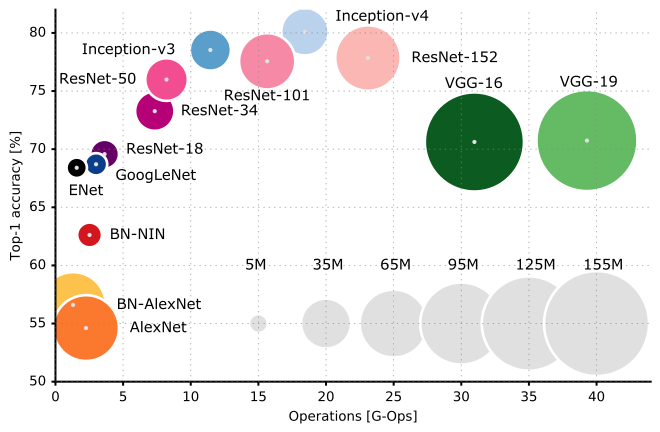
\includegraphics[resolution=100, scale=0.6]{architecturePerformance.png}
		\caption{Wydajność architektury względem ilości operacji potrzebnych do przejścia sygnału przez nią.}
\end{figure}


%\section{Przegląd efektywnych architektur}

\section{LeNet}
\begin{figure}[ht]
	\centering
			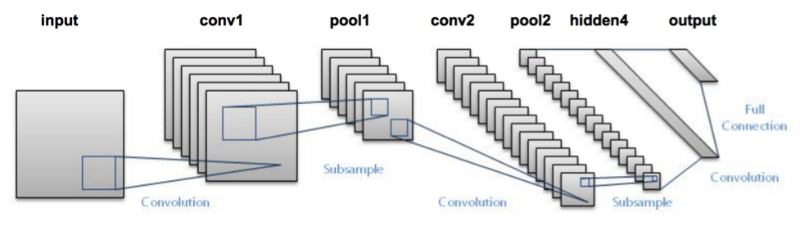
\includegraphics[resolution=100, scale=0.6]{LeNet.png}
		\caption{Architektura sieci LeNet}
\end{figure}

[Yann LeCun, Leon Bottou, Yoshua Bengio, Patrick Haffner, 1998] - Pierwsze praktyczne zastosowanie sieci konwolucyjnej do rozpoznawania cyfr. Sieć oparta o tą architekturę używana była do czytania kodów pocztowych, oraz krótkich ciągów liczb. Systemów implementujących LeNet używało około 10\% banków i instytucji pocztowych w Stanach Zjednoczonych Ameryki. Architektura została zaprezentowana w publikacji ''Gradient-Based Learning Applied to Document Recognition''.

Głównym przesłaniem publikacji jest pokazanie że systemy uczące lepiej nadają się do systemów rozpoznawania wzorców niż te polegające na opisywaniu wszystkich reguł. Używając najnowszych na te czasy osiągnięć uczenia maszynowego, autorzy prezentują w jaki sposób zastąpić ręcznie wykonane ekstraktory cech używając dobrze zaprojektowanego agenta, który pracuje wyłącznie w oparciu o piksele. Opierając się na paradygmacie programistycznym sieci transformatorowej, pozwalającej wszystkim modułom optymalizować kryteria wydajności dla całościowego zbioru domeny, wykluczono wszystkie reguły opisujące zbiór danych do rozpoznania.

Do czasu publikacji sieci LeNet, systemy rozpoznawania wzorców były budowane używając dwóch modułów. Pierwszy, ekstraktor cech, przekształcał sygnały wejściowe na wektory lub ciągi znaków złożone z symboli. Pozwalało to na łatwe porównywanie i łączenie elementów. Ekstraktor cech zawiera sztywne reguły, które są specyficzne dla zadania. Drugim elementem jest klasyfikator, moduł ogólnego przeznaczenia, podatny na uczenie. Główną bolączką takich systemów jest osoba projektująca zbiór cech. Jakość rozpoznawania wzorców bowiem zależy od kreatywności i ogromu pracy jaki włoży projektant pierwszego modułu w opisanie i rozpoznanie wszystkich możliwie występujących cech w zbiorze danych, na którym system ma pracować. Dodatkowo do tego podejścia zniechęca fakt, iż dla każdego innego systemu należy cechy projektować od początku. Nie ma znaczenia że dane wejściowe są bardzo podobne. Dla przykładu rozpoznawanie liter i cyfr, są tutaj rozpatrywane jako dwie zupełnie różne domeny, dla których należy zaprojektować osobne ekstraktory cech. Rozwiązaniem tych problemów jest ujednolicenie systemu i wyrzucenie modułu opierającego swoją wydajność na żmudnej pracy projektanta.

Lecun z zespołem, zaproponowali system oparty o ''gradientową propagację wsteczną''. Składa się ona z 7 warstw, bez wejściowej, ale licząc z wyjściową. Pełna nazwa LeNet-5. Liczba w nazwie oznacza ilość warstw ukrytych. Sieć w porównaniu z opisywanymi w następnych sekcjach jest najmniejsza (pamięciowo) i najprostsza w implementacji. Czas wytrenowania takiej sieci na nowoczesnym GPU zawiera się w mniej niż jednej minucie. Najlepszym zbiorem uczącym dla LeNet jest MINST, zbiór cyfr pisanych odręcznie, około 70 000 obrazów. Zbiór został przestudiowany przez wielu ekspertów od wizji komputerowej i jest to jeden z najstarszych zbiorów obrazów używanych do dziś w uczeniu maszynowym. Połączenie LeNet wraz z zestawem danych uczących MINST uchodzi za klasyczny wstęp do sieci neuronowych jako najprostszy przykład. Porównuje się je często do programów "Witaj, świecie!" w językach programowania.

Sieć na wejście przyjmuje sygnał złożony z obrazów 32x32 piksele w różnych odcieniach szarości (bez kolorów). Największa cyfra w bazie ma rozmiar 20x20 pikseli wyśrodkowane na polu o rozmiarach 28x28 pikseli. Wartości danych wejściowych są znormalizowane, wartość tła (białe piksele) wyrażona jest wartością -0,1, a wartość rozpoznawanych danych (czarne piksele) odpowiada wartości 1,175. Pozwala to uzyskać średnie wartości 0 i wariancje na poziomie 1, takie wartości znacząco przyspieszają proces uczenia. Używa filtra konwolucyjnego o rozmiarach 5x5 pikseli z przesunięciem o 1.

Pierwsza warstwa jest warstwą konwolucyjną w sześcioma mapami cech. Każdy neuron w mapie cech jest połączony do wejścia sąsiadującej drugiej warstwy o rozmiarach 5x5. Rozmiar każde mapy cech wynosi 28x28 pikseli, ma to zapobiegać wyjściem poza granice obrazu. Pierwsza warstwa zawiera 156 parametrów i aż 122 3 04 połączenia.

Druga warstwa jest przeznaczona do próbkowania i jak tak samo jak pierwsza, posiada 6 map cech o większym rozmiarze bo 14x14 pikseli. Każdy neuron w każdej z mapy cech jest połączony w sąsiedztwie rozmiarów 2x2 z cechą poprzedniej warstwy. Cztery wejścia do neuronu w drugiej warstwie są dodane, następnie mnożone przez współczynnik wag, na koniec wynik do wyniku operacji dodawany jest próg. Wynik podawany jest jako argument dla funkcji sygmoidalnej. Pola recepcyjne nie nachodzą na siebie, dlatego mapy cech są połowę mniejsze od tych w pierwszej warstwie. Druga warstwa ma 12 parametrów i już tylko 5 880 połączeń.

Trzecia warstwa jest warstwą konwolucyjną, tak samo jak pierwsza. Jest zaś większa od pierwszej i posiada 16 map cech. Każdy neuron w każdej mapie cech jest połączony do kilku sąsiadów o rozmiarach 5x5 pikseli w identycznych lokalizacjach podzbioru mapy cech drugiej warstwy. Nie łączy się wszystkich map cech drugiej warstwy z trzecią celem ograniczenia liczby parametrów oraz uniknięcia symetryczności sieci. Kiedy sieć nie jest symetryczna, każda mapa cech może nauczyć się zupełnie innych parametrów obrazu. Schemat połączeń działa następująco: pierwsze sześć map cech z warstwy trzeciej jest zasilanych wejściem z wyjścia kolejnych trzech map cech poprzedniej warstwy. Kolejne sześć wejść jest podłączonych do czterech wyjść z warstwy drugiej. Ostatnie wejście pobiera informację ze wszystkich sygnałów wyjściowych poprzedniej warstwy. Trzecia warstwa składa się z 1 516 parametrów i zawiera 151 600 połączeń.

Czwarta warstwa, jest tak samo jak druga, warstwą próbkowania złożoną z 16 map cech o rozmiarach 5x5 pikseli. Każda jednostka jest połączona w sąsiedztwo o rozmiarze 2x2 piksele z odpowiadającą mapą cech poprzedniej warstwy. Działa to identycznie jak łączenia między pierwszą a drugą warstwą. Czwarta warstwa składa się z 32 parametrów i zawiera 2 000 połączeń.

Piąta warstwa jest warstwą konwolucyjną ze 120 mapami cech. Każdy neuron jest połączony do sąsiedztwa 5x5 ze wszystkimi mapami cech z czwartej warstwy. Ponieważ poprzednia warstwa ma te same rozmiary, mapy cech w piątej warstwie będą rozmiarów 1x1, tworząc pełne połączenie między warstwami. Piąta warstwa złożona jest z 10 164 parametrów.

Szósta warstwa zrobiona jest z 84 neuronów w pełni połączonych z piątą warstwą. Składa się z 10 164 parametrów. Jest to tradycyjna warstwa złożona z prostych neuronów. Funkcję aktywacji tej warstwy pełni softmax, zwracająca na wyjściu rozkład prawdopodobieństwa dla każdej z klas.

Trenowanie sieci przy użyciu zestawu MINST (bez zniekształceń) pozwala zaobserwować, że funkcja błędu stabilizuje się dla zestawu uczącego i testowego po 12 przejściach przez sieć. Dodanie zniekształceń do zestawu treningowego (zwiększając jego ilość tysiąckrotnie) pozwoliło autorowi architektury na obniżenie błędu z 1\% do 0,8\%.

\begin{figure}[ht]
	\centering
			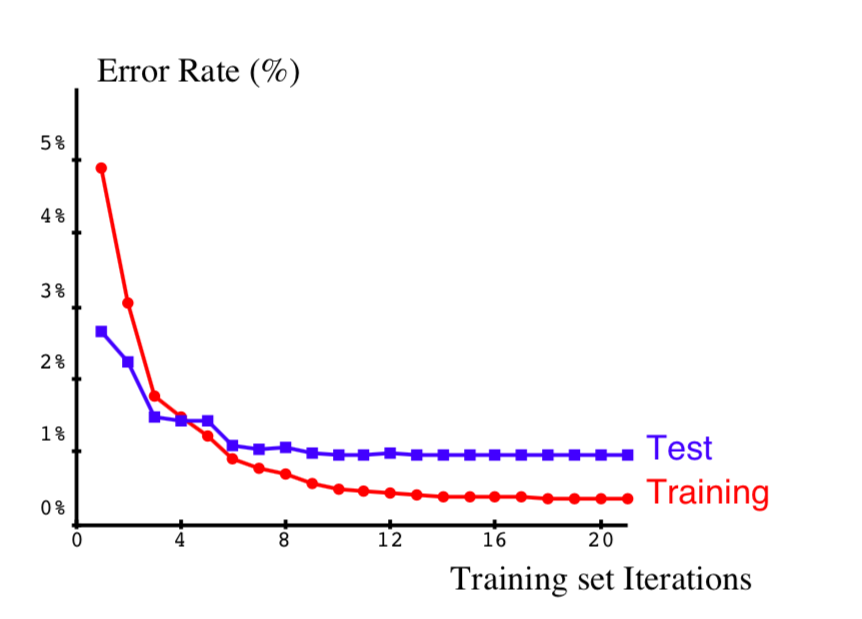
\includegraphics[resolution=100, scale=0.45]{leNetTraining.png}
		\caption{Współczynnik błędu po kolejnych iteracjach na zbiorze danych.}
\end{figure}


\section{AlexNet}
\begin{figure}[ht]
	\centering
			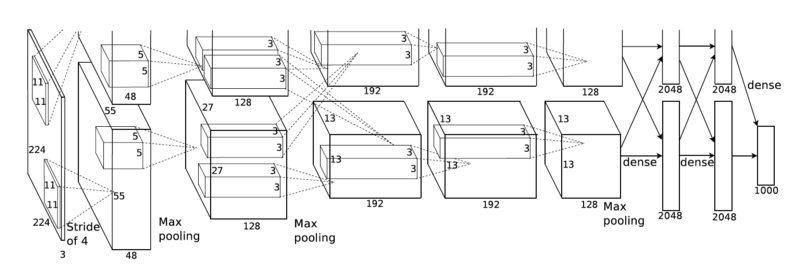
\includegraphics[resolution=100, scale=0.65]{AlexNet.png}
		\caption{Wizualizacja architektury sieci AlexNet}
\end{figure}

 [Alex Krizhevsky, Ilya Sutskever, Geoffrey E. Hinton, 2012] - pierwsza prawdziwa konwolucyjna sieć neuronowa (CNN), która pomogła zmienić opinię na temat uczenia głębokiego. Została zaimplementowana z użyciem biblioteki CUDA. Pierwsza sieć neuronowa, ucząca się z powodzeniem dla dużego zbioru danych.
 
 Została wytrenowana na zbiorze danych złożonym z ponad 15 milionów obrazów podzielonych na 22000 klas. 
 W testach top-1 i top-5 uzyskała wartości kolejno 37,5\% i 17\%, co pozwoliło wygrać konkurs ImageNet Large Scale Visual Recognition Challenge. 
 
 Sieć neuronowa zawiera 60 milionów parametrów i 650 000 neuronów. Architekturę tworzy 8 warstw, gdzie pierwsze 5 to warstwy konwolucyjne, a pozostałe 3 są warstwami w pełni połączonymi, ta ostatnia ma oczywiście 1000 wyjść z funkcji softmax. AlexNet znacząco przewyższyła swoją wydajnością poprzednich uczestników i wygrała zawody redukując błąd top-5 do 15,32\%. Drugie miejsce to błąd ok 26.2\% (nie była to CNN). Sieć jest głęboką modyfikacją architektury Yann’a LeCunn’a. AlexNet była zaplanowana na dwie karty graficzne, stąd rozdzielenie przepływu informacji na 2 części. Trenowanie sieci na 2 GPU było nowością na te czasy. Sieć została wytrenowana na zbiorze ImageNet. Do wyliczenia funkcji nieliniowych były używane ReLU (tutaj po raz pierwszy okazało się że ReLU działa dużo szybciej niż tangens hiperboliczny). Sieć o której obecnie uczy się studentów Data Science na lekcjach historii głębokich sieci neuronowych.
 
 Motywacja stojąca za stworzeniem tej przełomowej architektury była banalna: stworzyć narzędzie pozwalające uczyć oprogramowanie na dużych zbiorach danych.
 Wcześniejsze podejście wykorzystywało metody uczenia maszynowego na małych zbiorach, liczonych w dziesiątkach tysięcy obrazów. Rozpoznanie prostych kategorii w małych bazach było o tyle proste że nie odpowiadało różnym sytuacjom spotykanym w życiu codziennym, gdzie obiekty są ujęte w różnych proporcjach, rozmiarach, umieszczeniu na zdjęciu. Różność w szczegółach prawdziwych obiektów (np. kolor i typ ubrania na człowieku) również uniemożliwiają uczenie na starych zasadach. Aby wyuczyć program ponad 22 000 kategorii w 15 milionach zdjęć, z konkursu ImageNet należało stworzyć nową architekturę, zdolną przetworzyć tak duży zbiór danych.
 
 Wybór padł na splotowe sieci neuronowe. Są dużo mniej złożone obliczeniowo od klasycznych w pełni połączonych sieci neuronowych i mają wystarczająco dobrą wydajność w klasyfikacji obrazów. Autorzy zdecydowali się napisać własną implementację konwolucji dwuwymiarowej i pozostałych operacji trenowania sieci, zoptymalizowane do pracy na procesorach graficznych używających CUDA. Po zastosowaniu wszystkich znanych w tym czasie metod zapobiegania przeuczenia oraz złożeniu pięciu warstw konwolucyjnych z trzema w pełni połączonymi warstwami, otrzymano architekturę wydajnościowo ograniczoną tylko pamięcią operacyjną kart graficznych i czasem oddanym na trening. W konkluzji Hinton sugeruje, że szybsze karty graficzne i większe zbiory danych pozwolą sukcesywnie zwiększać wydajność jego architektury.
 
 Architektura sieci złożona jest z ośmiu warstw uczących, podzielonych na pięć konwolucyjnych i trzy w pełni połączone oraz warstwę wyjściową złożoną z 1000 neuronów produkujących prawdopodobieństwo dla każdej z klas, za pomocą funkcji $softmax$. Sieć ma na celu maksymalizację regresji logistycznej, czyli zmaksymalizować średnią ze wszystkich sygnałów treningowych oraz przypisać każdej z nich prawdopodobieństwo rozpoznania poprawnej klasy.
  W samym ułożeniu warstw nie ma nic nowatorskiego względem LeNet5, różnice pojawiają się w implementacji mechanizmów uczenia.
 \begin{itemize}
 \item Nieliniowość ReLU -- zmiana używanej wcześniej w każdej sieci, funkcji tangensa hiperbolicznego na rektyfikowaną jednostkę liniową. Sam zabieg zmiany funkcji aktywacji pozwala na wielokrotnie krótszy czas uczenia.
 \item Trening na wielu kartach graficznych -- operowanie na 1,2 miliona zdjęć uczących wymaga sporych zasobów pamięciowych. Dlatego wykorzystano najmocniejsze na ten czas karty graficzne dostępne na rynku dla graczy i połączono je układem SLI. Układ ten pozwala na czytanie z rejestrów pamięci drugiej karty z pominięciem procesora komputera. Trening architektury przygotowanej dla dwóch kart graficznych zmniejszył czas treningu, który byłby trochę wyższy gdyby architekturę pozostawić domyślną, jednoprocesorową.
 \item Nachądzące warstwy łączące -- zastosowano tutaj sztuczkę stosowaną obecnie w każdej sieci konwolucyjnej. Zmniejszając rozmiar siatki w warstwie łączącej poniżej rozmiarów sąsiedztwa które łączy, następuje zjawisko nachodzącego się na siebie łączenia cech z warstwy poprzedniej. Pozwala to na zmniejszenie możliwości przeuczenia modelu.
 \end{itemize}
 
 Połączenia między warstwami, widoczne na załączonym rysunku, prezentują się następująco. Neurony z drugiej, czwartej oraz piątej warstwy konwolucyjnej są połączone do neuronów warstwy poprzedniej położonych na tym samym GPU. Ukazuje to jak bardzo sieć ta jest zależna od sprzętu. Neurony z trzeciej warstwy są połączone ze wszystkimi neuronami z drugiej warstwy. Jednostki w warstwach w pełni połączonych są połączone ze wszystkimi jednostkami z warstwy poprzedniej. Za pierwszą i drugą warstwą konwolucyjną ustawione są warstwy normalizujące syngał wyjściowy. Warstwy łączące odbierają sygnał od warstw normalizujących. Każdy neuron z warstw konwolucyjnej oraz w pełni połączonej jest wyposażony w rektyfikowaną jednostkę liniową jako funkcję aktywacji.

Rozmiary warstw oraz ilość parametrów są oszczędne w porównaniu z dzisiejszymi architekturami. Pierwsza warstwa konwolucyjna posiada wejście rozmiarów 224x224x3 pikseli (obrazy w ImageNet są kolorowe), przekazywane do 96 neuronów o rozmiarach 11x11x3 z przesunięciem wynoszącym 4 piksele. Druga warstwa konwolucyjna, odbiera obraz po łączeniu. Wartości są przetwarzane przez 256 neuronów o rozmiarze 5x5x48, 48 map cech, każda złożona z 25 pikseli. Trzecia, czwarta i piąta warstwa konwolucyjna są połączone ze sobą bez jakichkolwiek pośredników w rodzaju warstw łączących i normalizujących. Trzecia warstwa konwolucyjna złożona jest z 384 neuronów o rozmiarach 3 x 3 x 256, połączona pośrednio z drugą warstwą konwolucyjną przez normalizacje syngału i warstwę łączenia. Czwarta warstwa konwolucyjna również jest złożona z 384 jednostek, jednak ilość map cech, ogranicza się do 192. Ostatnia warstwa konwolucyjna ma 256 jednostek o rozmiarze 3 x 3 x 192 (tak samo jak czwarta). Ostatnie, w pełni połączone warstwy są identyczne, każda ma 4096 neurnów. Całość złożona jest z 60 milionów parametrów. \cite{NIPS2012_4824}

\section{VGG Net}
\begin{figure}[ht]
	\centering
			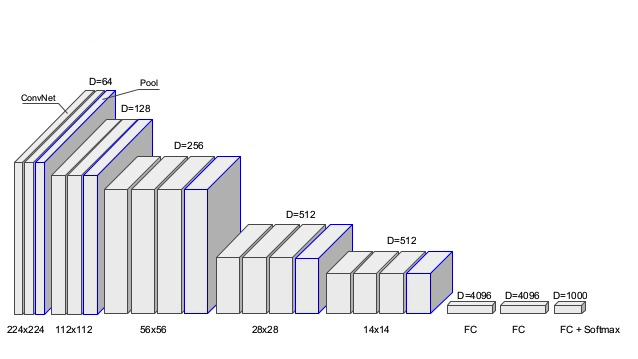
\includegraphics[resolution=100, scale=0.8]{VGGarchitecture.png}
		\caption{Klasyczna architektura sieci VGG-16}
\end{figure}

 [Simoyan i Zisserman, 2015] - %sieć złożona z 16 warstw konwolucyjnych, która charakteryzuje się małymi filtrami i dużą głębokością sieci.
%W trakcie trenowania sieci wyjście jest ustawione na ustalony rozmiar (224 x 224 x 3). Przetwarzanie wstępne obejmuje odjęcie mediany wartości RGB dla każdego piksela. Zdjęcie jest przetwarzanie przez stos warstw konwolucyjnych, gdzie używane są filtry o bardzo małym polu widzenia (3x3) [najmniejszy możliwy rozmiar by móc rozpoznać kierunek]. Operacja Max-pooling jest wykonana na polu 4 pikseli, co pokazuje że jest to pobieranie jak najmniejszych cech z obrazu. Ukryte warstwy są wyposażone w nieliniową funkcję aktywacji ReLU. Po stosie warstw konwolucyjnych, następuje nałożenie 3 warstw w pełni połączonych (to takie duże warstwy zawierające wszystkie cechy?). Pierwsze dwie mają 4096 kanałów, trzecia już tylko 1000 (po jednym kanale na klasę obiektu). Obecnie architektura ta jest dość popularnym wyborem dla wyodrębniania cech ze zdjęć. Konfiguracje wag dla zbioru obrazów z ImageNet są dostępne online. W tej sieci problemem jest 140 milionów parametrów, którymi czasem trzeba zarządzać. 
Sieć jest wielokrotnie bardziej złożona obliczeniowo od AlexNet, że posiadając cztery karty graficzne NVIDIA Titan Black (10-krotnie więcej mocy niż dwie karty GeForce 580 GTX), wytrenowanie pojedynczej sieci zajęło ponad dwa tygodnie.

Sygnały wejściowe dla sieci skomponowane są z obrazów o stałym rozmiarze 224 x 224 x 3 pikseli. Zdjęcia są przesyłane przez stos warstw konwolucyjnych z filtrami o małych rozmiarach 3 x 3 piksele. W jednej z dostępnych konfiguracji używane są filtry o rozmiarze 1 x 1, które służą wyłącznie przekształceniu liniowemu kanałów wejściowych. Przesunięcie konwolucyjne jest ustawione sztywno na jeden piksel, podobnie jak w AlexNet, występuje tutaj nachodzenie warstw łączących. Tak małe przesunięcie pozwala zachować cechy przestrzenne obrazu po konwolucji. Pięć warstw łączących wykorzystuje metodę Max-Pooling na oknie rozmiarów 2 x 2 piksele z przesunięciem o 2 piksele.

Warstwy konwolucyjne różnią się głębokością, między kolejnymi implementacjami architektury VGG. W każdej z nich jednak umieszczone są na stosie, po którym następują zawsze trzy warstwy w pełni połączone. Pierwsze dwie warstwy połączone mają razem 8192 neuronów (4096 na warstwę), trzecia oczywiście złożona jest z 1000 jednostek, ponieważ tyle klas przewiduje zbiór ILSVRC. Mapy cech rosną wgłąb sieci, zaczynając od 64 na pierwszej warstwie konwolucyjnej i podwajają szerokość z każdą warstwą łączącą do osiągnięcia 512 filtrów. Ilość parametrów waha się od 133 milionów do 144 milionów w zależności od konfiguracji sieci.

Wszystkie warstwy ukryte korzystają z rektyfikowanej jednostki liniowej jako funkcji aktywacji.

Rozdział testujący wydajność architektur, przedstawia sieć neuronową w wariancie 19 warstwowym (16 warstw konwolucyjnych, oraz 3 w pełni połączone).

W tej architekturze również widać jej wiekowość. Najbardziej wymyślna i skomplikowana konfiguracja sieci jest powolna i nie klasyfikuje zbyt dobrze obrazów. Błędy plasują się następująco:
\begin{itemize}
\item Top-1 23,7\%,
\item Top-5 6,8\%.
\end{itemize}
\cite{DBLP:journals/corr/SimonyanZ14a}

\begin{figure}[ht]
	\centering
			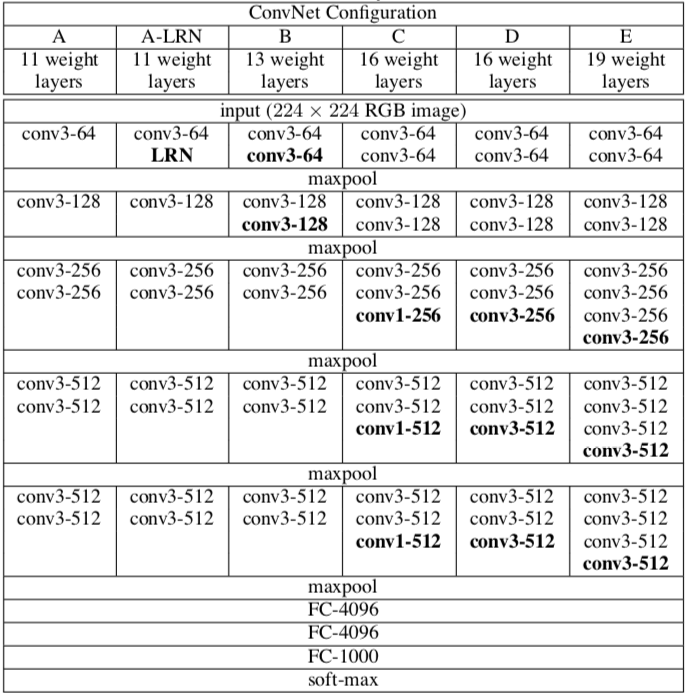
\includegraphics[resolution=100, scale=0.8]{vggArchComparison.png}
		\caption{Porównanie architektury warstwowej różnych konfiguracji VGG}
\end{figure}


\section{GoogLeNet}
\begin{figure}[h]
	\centering
			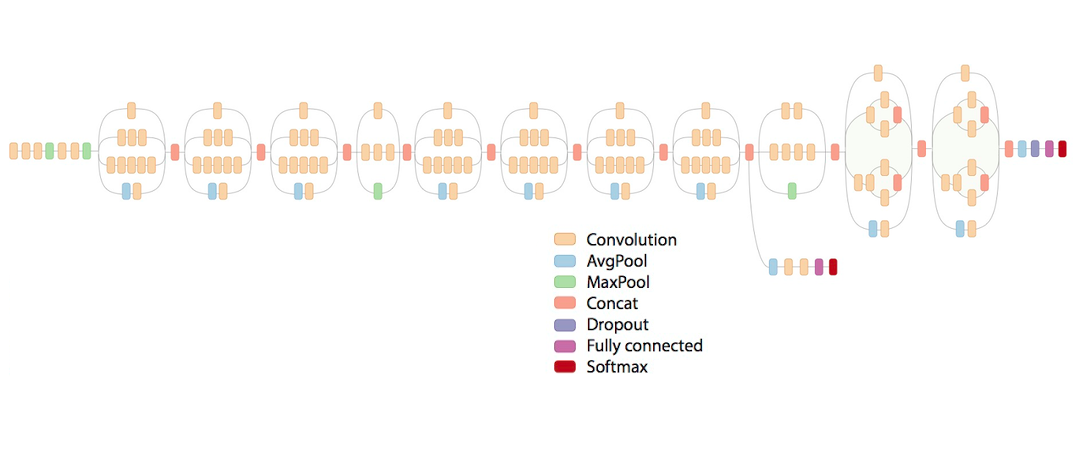
\includegraphics[resolution=100, scale=0.36]{inceptionv3architecture.png}
		\caption{Architektura sieci Inception v3}
\end{figure}

\begin{figure}[ht]
	\centering
			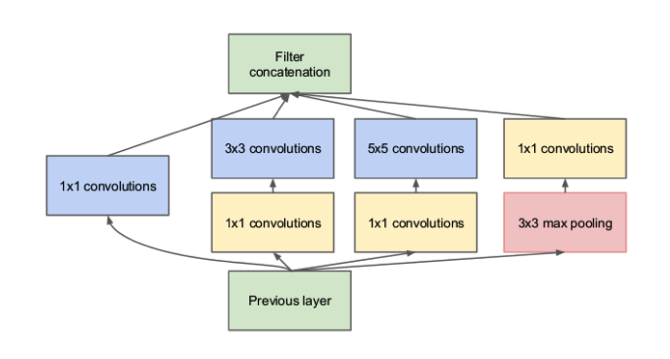
\includegraphics[resolution=100, scale=0.7]{inceptionModule.png}
		\caption{Moduł Incepcja}
\end{figure}

[Christian Szegedy, Wei Liu, Yangqing Jia, Pierre Sermanet, Scott Reed, Dragomir Anguelov, Dumitru Erhan, Vincent Vanhoucke, Andrew Rabinovich, 2014] -- produkt jak nazwa wskazuje wyszedł z firmy Google. Częściej używana nazwa Incepcja wywodzi się częściowo z nazwy filmu Christophera Nolana. Inspiracją jest mem internetowy ''wchodzenie głębiej w konwolucje''. Analogia do schodzenia w kolejne warstwy podświadomości.\cite{siteDeeper}

Sieć charakteryzuje przełomowa poprawa wykorzystania zasobów wewnętrznych. GoogleNet jest zaprojektowana na jak największą szerokość i głębokość, co ma jej zapewnić świetną wydajność uczenia, jednocześnie utrzymując użycie mocy obliczeniowej na stałym poziomie. Autorzy w publikacji dotyczącej działania sieci chwalą się, że ich architektura ma aż 12 razy mniej parametrów niż zwycięzca z ImageNet 2012 (mowa o AlexNet), jednocześnie będąc zdecydowanie dokładniejszym klasyfikatorem. Ograniczenie obliczeniowym w postaci 1,5 miliarda mnożeń i dodawań, jakie zostało narzucone na autorów jest wymuszenie możliwości praktycznego użycia modeli opartych o tą architekturę. Kolejnym rozważnym elementem dlaczego wymagania pamięciowe modelu sieci są tak istotne, jest rosnąca popularność inteligentnych aplikacji mobilnych. Każda aplikacja może być wyposażona w specjalistyczny model wspomagający działanie, nie można jednak zakładać nieskończonej ilości pamięci, bo te telefony mają ograniczone. Należy się tutaj również liczyć z ilością przesyłanych danych komórkowych. Sieć złożona jest z tylko 22 warstw.

Wprowadzona idea organizacji grup warstw w moduły jest przełomowe w sposobie, w jaki postrzega się sieci neuronowe. Do tej pory był to zbiór neuronów podzielonych na warstwy, dodanie jednostki zwanej modułem, tworzy abstrakcje wykraczające na wyższy stopień. Świadczy to o wielkości zasobów obliczeniowych dostępnych w dopiero ostatnich latach.

Motywacją do wprowadzenia warstwy incepcji jest umożliwienie pokrycia jak największej powierzchni zdjęcia i utrzymanie dobrej rozdzielczości małych cech obrazu. Moduł ma za zadania wykonać równoległą konwolucję w różnych rozmiarach, od 1x1 do 5x5. Zastosowanie kilku filtrów Gabora o różnych rozmiarach daje możliwość rozpoznania wielu obiektów w różnej skali. W przedstawionej architekturze znajduje się 9 modułów incepcji. Celem uniknięcia zbyt wielkiej ilości parametrów zastosowano techniki wąskiego gardła. Używając konkatenacji parametrów można zbudować moduł incepcji z większą ilością przekształceń nieliniowych, wykorzystując mniejszą liczbę parametrów. Warstwa łącząca dodawana jest na koniec modułu aby zsumować wartości z poprzednich warstw. Konkatenacja odbywa się przez ułożenie szeregowe wartości z filtrów wszystkich wielkości.


%Optymalizacja jakości opiera się na zasadzie Hebbian’a (jest to teoria neuronauki, która mówi o adaptacji neuronów w trakcie nauki). Błędy klasyfikacji wynoszą top-1: 17,2\% i top-5: 3,58\% (dla v3). Sieć składa się łącznie z 22 warstw. Sieć jest modułowa, gdzie każdy moduł pełni rolę wielopoziomowego ekstraktora cech przeliczającego konwolucje na macierzach rozmiarów 1x1, 3x3, 5x5. Zaletą tej architektury są bardzo małe rozmiary wag (mniej niż 100MB dla v3). Kolejną ważną zaletą jest ilość parametrów, tylko 4 miliony co jest wynikiem 12 razy lepszym od AlexNet. Jest to jedna z najbardziej złożonych sieci względem architektury modułowej. W wersji naiwnej każda warstwa posiada 4 ekstraktory cech (3 konwolucyjne i jedną 3x3 max pooling), następnie wartości te są składane i wysyłane do warstwy wyżej. Do poprawienia wydajności obliczeniowej pozbyto się warstwy “w pełni połączonej”. 

\cite{DBLP:journals/corr/SzegedyLJSRAEVR14}

\section{ResNet}
\begin{figure}[ht]
	\centering
			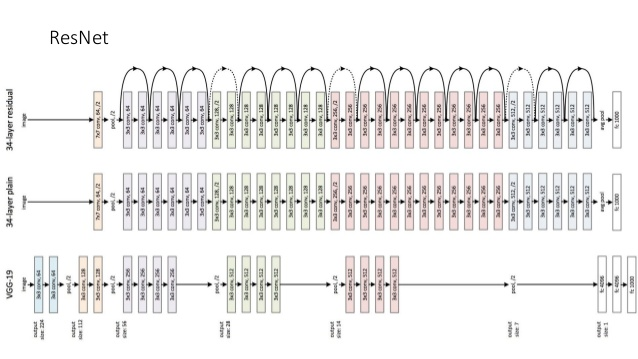
\includegraphics[resolution=100, scale=0.5]{ResNet.png}
		\caption{Architektura sieci ResNet}
\end{figure}

[Kaiming He, Xiangyu Zhang, Shaoqing Ren, Jian Sun, 2015] -- architektura oparta została na mikro modułach. Ze względu na trudności pojawiające się w uczeniu bardzo głębokich sieci neuronowych (długi czas nauczania, łatwość przeuczenia), zespół badaczy z Microsoftu zaproponował szczątkowe uczenie w bardzo głębokich sieciach. 
%Charakteryzuje się możliwością odrzucania połączeń i posiada ogromny moduł na normalizację zbioru iteracji (ang. batch normalization). Normalizacja jest pomysłem zaczerpniętym z rekurencyjnych sieci neuronowych. Ta technika pozwala stworzyć sieć ze 152 warstwami ukrytymi przy zachowaniu złożoności mniejszej niż VGG. 

\cite{DBLP:journals/corr/HeZRS15}


%\section{ResNeXt}
%\begin{figure}[h]
%	\centering
%			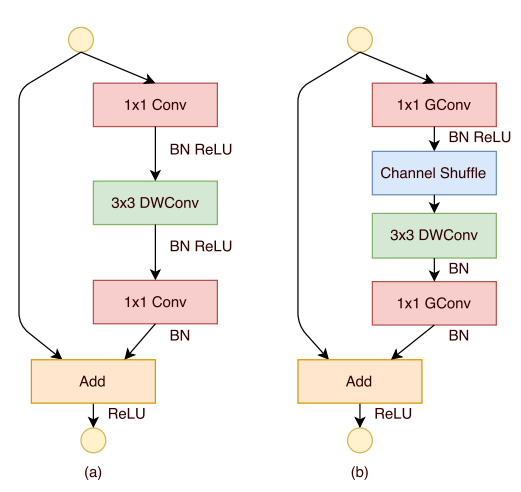
\includegraphics[resolution=100, scale=0.9]{ResNeXt.png}
%		\caption{Architektura modułu sieci ResNeXt}
%\end{figure}
%\cite{DBLP:journals/corr/XieGDTH16}

%[Saining Xie, Ross Girshick, Piotr Dollar Zhuowen Tu Kaiming He, 2017] - modularyzowalna 
%\cite{DBLP:journals/corr/abs-1805-08700}

\section{YOLO - You Only Look Once}
\begin{figure}[ht]
	\centering
			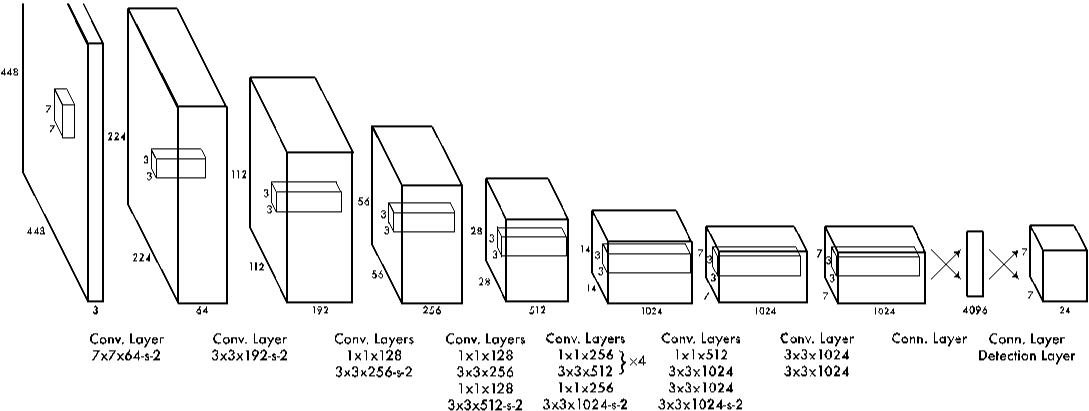
\includegraphics[resolution=100, scale=0.5]{YOLO.png}
		\caption{Wizualizacja architektury sieci YOLO}
\end{figure}

[Joseph Redmon, Santosh Divvala, Ross Girshick, Ali Farhadi, 2016] - You Only Look Once jest systemem wykrywania obiektów w czasie rzeczywistym. Obraz jest dzielony na części oddzielonymi od siebie prostokątami.
Cały przepływ danych do wykrycia obiektów jest jedną siecią, dlatego może być zoptymalizowany \cite{DBLP:journals/corr/RedmonDGF15}


\section{SqueezeNet}
\begin{figure}[ht]
	\centering
			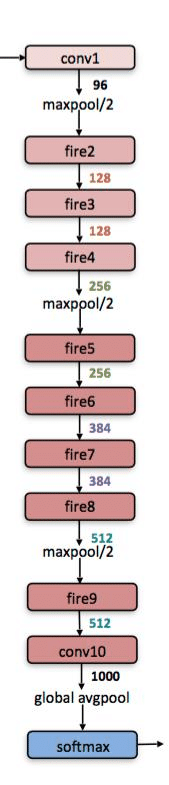
\includegraphics[resolution=100, scale=0.65]{SqueezeNet.png}
		\caption{Architektura sieci SqueezeNet}
\end{figure}
[Forrest N. Iandola, Song Han, Metthew W, Moskewicz, Khalid Ashraf, William J. Dally, Kurt Keutzer, 2016] -- SqueezeNet jak nazwa sugeruje jest siecią, która z założenia ma składać się z niewielkiej ilości parametrów i dzięki temu wyprodukować niewielki model. Już w tytule publikacji opisującej sieć, autorzy porównują dokładność sieci do AlexNet, zdradzając przy tym jej rozmiar wynoszący mniej niż 0,5MB. Głównym przeznaczeniem tak małej sieci jest dostarczenie wystarczająco dobrej wydajności, na poziomie najlepszych sieci z ostatnich dwóch do trzech lat. Sieć z założenia ma być mała, ma to na celu wyłuskać trzy zalety:
\begin{itemize}
\item ograniczyć komunikację między serwerami podczas treningu. Szczególnie przydatna cecha jeśli trening odbywa się na rozproszonym fizycznie środowisku. Korzystając z przeglądarek użytkowników oraz urządzeń mobilnych można trenować model tylko jeśli nie wymaga on ciągłej komunikacji między wszystkimi urządzeniami.
\item ograniczyć ilość transferu potrzebnego na eksport i aktualizacje modelu z chmur do urządzeń mobilnych. W szczególności kiedy sieć urządzeń, np. autonomiczne samochody, wymagają aktualizacji w czasie rzeczywistym w nieznanych warunkach zasięgu telekomunikacji.
\item umożliwić wdrożenie na bezpośrednio programowalnej macierzy bramek i innych urządzeniach wdrażanych w ramach IoT. Urządzenia te mają często do dyspozycji mniej niż 10MB pamięci, dlatego standardowe modele (zawierające powyżej 250MB) nie sprawdzą się.
\end{itemize}

SqueezeNet budowany jest wielu jednostek nazywanych ''modułami ognia''. 
W celu znalezienia optymalnej architektury autorom przyświecały trzy strategie:
\begin{itemize}
\item Zmniejszono rozmiar filtra z 3x3 pikseli do 1x1 piksel.
\item Zmniejszono ilość kanałow wejściowych do filtrów o rozmiarze 3x3 piksele. Używa się warstw ściskających do ograniczenia ilości kanałów podpiętych pod te filtry.
\item Opóźniono zmniejszenie rozdzielczości zdjęcia, aby dać warstwą konwolucyjnym większe mapy aktywacji. Standardowo próbkowanie odbywa się przez zwiększenie przesunięcia pola receptywnego powyżej jednego piksela. W tej architekturze zwiększanie przesunięcia pola receptywnego w głąb sieci pozwoli zwiększyć dokładność klasyfikacji bez wpływu na pozostałe parametry. Ta technika ma na celu utrzymanie wydajności w klasyfikacji przy zmniejszonej liczbie parametrów.
\end{itemize}

''Moduł ognia'' to zbiór warstw i operacji. Na jeden moduł składa się \textit{warstwa konwolucyjna ściskająca} z filtrami o rozmiarze 1 x 1 piksel. Warstwa ściskająca ogranicza ilość dużych filtrów, przepuszczając te o rozmiarze jednego piksela. Sygnały z tej warstwy są przekazywane do warstwy rozszerzającej. Ta warstwa zawiera kilka filtrów konwolucyjnych 1 x 1 oraz 3 x 3 piksele. 

Pierwsza warstwa sieci jest warstwą konwolucyjną o rozmiarach 111x111x96 (14 208 parametrów), liczba parametrów jest istotna ponieważ są one przycinane po każdym module ognia, nie wylicza się ich tutaj przez mnożenie rozmiarów okna. Następnie ustawionych jest osiem modułów ognia. Początkowo ilość filtrów wynosi 128 i jest zwiększana w głąb sieci, filtry są wyposażone w margines mający na celu poszerzyć moduły. Po przejściu przez ogień, sygnał jest przepuszczany przez ostatnią warstwę konwolucyjną. Sieć jest wyposażona w warstwy łączące używając funkcji $max()$ z przesunięciem wynoszącym 2 piksele. Warstwy łączące ustawione są na wyjściu warstw: pierwszej, czwartej, ósmej, dziesiątej. Rolę funkcji aktywacji pełni rektyfikowana jednostka liniowa. Rozmiary filtrów modułów ognia rośnie następująco:
\begin{itemize}
\item Moduł 1: 55x55x128 (5 746 parametrów),
\item Moduł 2: 55x55x128 (6 258 parametrów), 
\item Moduł 3: 55x55x256 (20 646 parametrów),
\item Moduł 4: 27x27x256 (24 742 parametrów),
\item Moduł 5: 27x27x384 (44 700 parametrów),
\item Moduł 6: 27x27x384 (46 236 parametrów),
\item Moduł 7: 27x27x512 (77 581 parametrów),
\item Moduł 8: 13x13x512 (77 581 parametrów),
\end{itemize}
Dodatkowo ostatni moduł ognia (dziewiąta warstwa), wyposażony jest w mechanizm odrzucania części sygnałów (ang. dropout). Sygnały z ostatniej warstwy ognia przechodzą przez jeszcze jedną warstwę konwolucyjną rozmiarów 13x13x1000 (szerokość wyznaczona ilością klas).
Zakończenie sieci wyliczane jest przez funkcję liczącą średniej z warstwy łączącej. Ta wartość jest przekazywana do warstwy wyjściowej, wyliczającej softmax dla wszystkich z 1000 klas. Zakończenie sieci nie różni się od pozostałych architektur konwolucyjnych.

Różnicą szczególnie widoczną względem pozostałych sieci splotowych jest brak jakiejkolwiek warstwy w pełni połączonej. Jest to świadomy wybór. Warto zaznaczyć podejście autorów do ograniczenia rozmiarów sieci nie ogranicza się na samej architekturze. Rejestry pamięci zostały przycięte do 6 bitów redukując tym samym rozmiar dziesięciokrotnie. Rysunek z porównaniem rozmiaru modeli przy różnych stopniach kompresji udowadnia, że wraz z kompresją nie trzeba tracić na jakości, wręcz przeciwnie, przy prawidłowej architekturze dokładność może być wyższa niż w innych rozbudowanych architekturach. \cite{DBLP:journals/corr/IandolaMAHDK16}

\begin{figure}[ht]
	\centering
			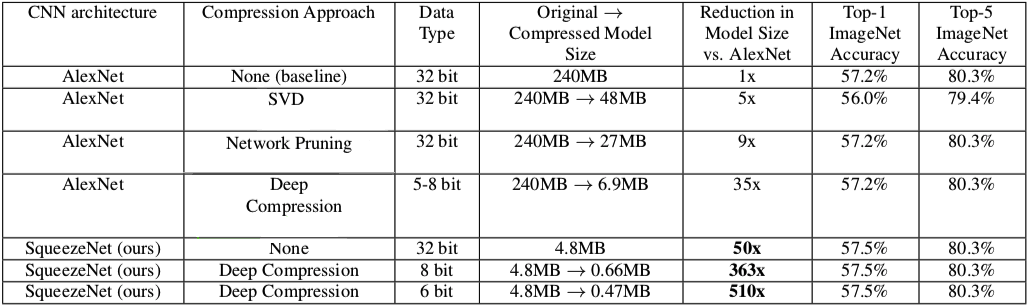
\includegraphics[resolution=100, scale=0.55]{squeezeNetCompression.png}
		\caption{Porównanie rozmiarów modelu dla architektur SqueezeNet i AlexNet. (z publikacji IandolaMAHDK16)}
\end{figure}

\subsection{SegNet}
\begin{figure}[ht]
	\centering
			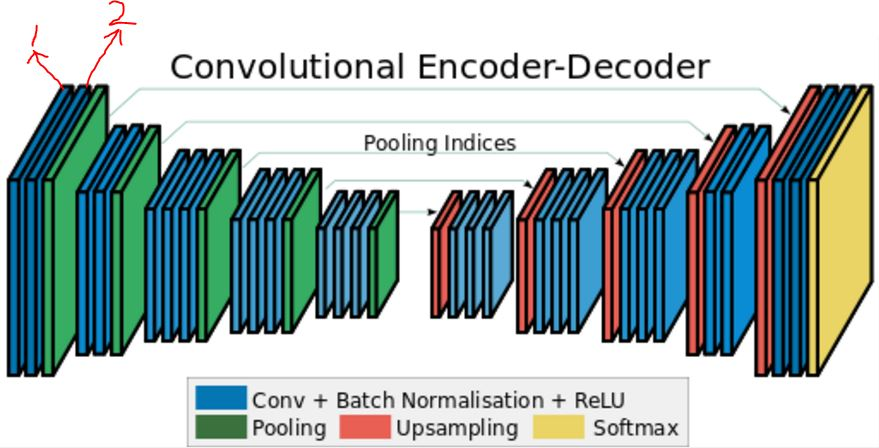
\includegraphics[resolution=100, scale=0.4]{SegNet.png}
		\caption{Wizualizacja architektury sieci SegNet}
\end{figure}
[Vijay Badrinarayanan, Alex Kendall, Roberto Cipolla, 2016] -- rozwinięcie nazwy to ''Segmentation Network'' sugeruje zastosowanie sieci. Została zaprojektowana do dzielenia obrazu na segmenty definiujące rozpoznany obiekt. Do segregacji zastosowano architekturę koderów i dekoderów. Jest to nowatorskie podejście do ułożenia sieci. Silnik segmentacji złożony jest z sieci koderów oraz dekoderów, na wyjściu znajduje się warstwa klasyfikacji oparta o semantykę pikseli. Topologicznie, architektura kodera jest kopią warstw konwolucyjnych opisywanej wcześniej sieci VGG. Dekoder w sieci zajmuje się mapowaniem zakodowanych map cech o niskiej rozdzielczości na mapy cech o wysokiej rozdzielczości (identycznej do sygnału wejściowego). Nowością w SegNet jest sposób w jaki dekoder zwiększa rozdzielczość sygnałów wejściowych zawierających mapy cech. Dokładniej dekoder używa łączenia indeksów, wyliczanego w warstwie łączącej, dając przekształcenie nieliniowe. Dzięki temu pomija się potrzebę dodatkowego uczenia sieci w jaki sposób ma skalować rozdzielczość. Mapy poddane próbkowaniu są rzadkie i poddane konwolucji celem wyprodukowania gęstych map cech.

Segnet ma w założeniu być podstawą aplikacji mających zrozumienie przedstawianego obrazu. Bardzo ważnym aspektem projektowym jest wydajność pamięciowa i czas potrzebny na rozpoznanie obiektów po treningu, powinno się to odbywać w czasie rzeczywistym.

Architektura podzielona jest na trzy części:
\begin{itemize}
\item podsieć kodująca,
\item podsieć dekodująca,
\item warstwa klasyfikacji.
\end{itemize}

Pierwsza podsieć złożona jest z 13 warstw splotowych, skopiowanych z sieci VGG16 przedstawionej we wcześniejszej sekcji. Taki układ umożliwia przeniesienie zestawu wag z wytrenowanych już modeli na wielkich zbiorach danych. W pełni połączone warstwy zostały całkowicie porzucone na rzecz uczenia map cech z wysoką rozdzielczością na najgłębszym (w ostatniej warstwie) wyjściu kodera. Zabieg ten zmniejsza ilość parametrów prawie dziesięciokrotnie, w porównaniu z innymi architekturami o podobnej złożoności. Wszystkie warstwy kodujące posiadają swoje odpowiedniki w warstwach dekodujących. Ostatnie wyjście warstwy dekodującej jest przekazane do klasyfikatora soft-max (jak każda sieć neuronowa), który zwraca prawdopodobieństwo wystąpienia klasy w każdym pikselu z osobna.
Każda warstwa kodująca w sieci wykonuje konwolucje na banku filtrów, które następnie po utworzeniu map cech zostają znormalizowane. Znormalizowane mapy cech zostają przeliczone przez funkcję aktywacji ReLU. Po każdej warstwie kodującej następuje warstwa łącząca MaxPooling z rozmiarem okna 2 x 2 piksele i przesunięciem o 2 piksele (okna na siebie nie nachodzą). Warstwa łącząca zapobiega zmianom przy niewielkich przesunięciach przestrzennych obrazu. Próbkowanie, które następuje zaraz za warstwą łączącą, zwraca kontekst w obrazie, z osobna dla każdego pliku.

Ze względu na konieczność wykrywania brzegów każdego elementu, autorzy wystrzegają się wszelkich rozwiązań wytracających szczegóły krawędzi. Przechwycenie i przechowanie informacji o krawędziach obiektu musi nastąpić w koderze map cech przed wykonaniem próbkowania. Proponowanym rozwiązaniem, z zachowaniem oszczędności pamięci jest zapamiętanie indeksów z warstwy łączącej. W ten sposób lokalizacje są przechowywane tylko dla wartości maksymalnych z każdego obszaru pola receptywnego, zachowując największe różnice ilość pamięci jest ograniczona czterokrotnie bez narażania się na znaczącą utratę jakości. Przechowując tak małą ilość danych, w architekturze zdecydowano się na użycie dwóch bitów na każde pole łączące (zamiast standardowego 32 bitowego pola zmiennoprzecinkowego).

Dekodery w sieci skalują mapę cech, którą dostają na wejście używając zapisanych wcześniej indeksów z warstwy łączącej. Dekoder mając te informacje tworzy rzadką mapę cech. Po utworzeniu map cech, dekoder przekazuje wyniki do konwolucji z bankiem filtrującym dekodera. Wynikiem splecenia jest normalna gęsta mapa cech. Każda z nowo utworzonych map jest poddawana procesowi normalizacji. Pierwszy dekoder tworzy wielokanałową mapę cech, mimo że odpowiadający mu dekoder posiada tylko 3 kanały (te z obrazu na wejściu). Jest to jedyny dekoder, który nie posiada tej samej ilości kanałów co odpowiadający mu koder.

Lista cech złożona z wielowymiarowego tensora, jest przekazywana z ostatniego dekodera do warstwy zawierającej klasyfikator z funkcja aktywacji soft-max. Jak już wcześniej wspomniano, każdy piksel otrzymuje własną klasyfikację. Wartością wyjściową tej warstwy jest obraz o ilości kanałów równej ilości klas, z aktywnym kanałem klasy o najwyższym prawdopodobieństwie na każdym z pikseli.

\cite{DBLP:journals/corr/BadrinarayananH15}

\section{Generative Adversarial Network}
\begin{figure}[ht]
	\centering
			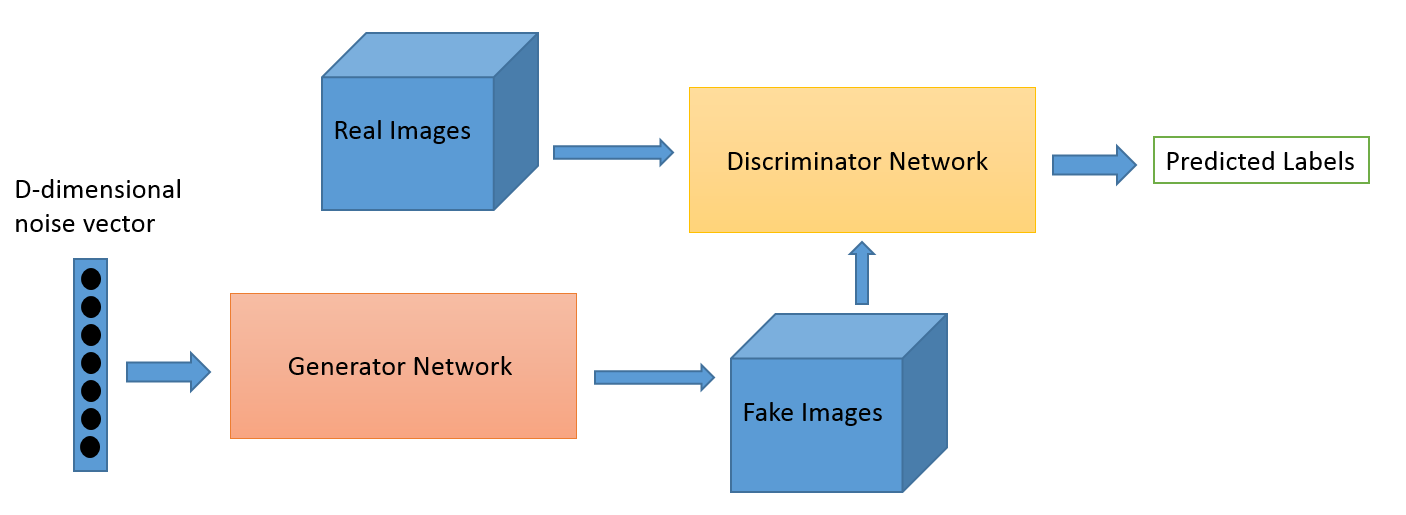
\includegraphics[resolution=100,scale=0.36]{GAN.png}
		\caption{Wysokopoziomowe moduły sieci GAN}
\end{figure}

[Ian J. Goodfellow, Jean Pouget-Abadie, Mehdi Mirza, Bing Xu, David Warde-Farley, Sherjil Ozair, Aaron Courville, Yoshua Bengio, 2014] Zupełnie inny typ sieci od pozostałych. Opiera się o zamysł dwóch sieci, traktowanych jako przeciwnicy. Pierwsza sieć generująca model, zwana generatorem G, tworzy swoje wyjście na podstawie rozkładu danych uczących. Druga sieć, model rozróżniający, znany jako dyskryminator D, którego zadaniem jest oszacowanie prawdopodobieństwa że sygnał otrzymany na wejściu pochodzi z danych treningowych a nie z generatora. Zadaniem G jest wytwarzać dane zmuszające sieć D do pomyłki. Jest to odpowiednik algorytmu min-max, czyli metodzie minimalizowania maksymalnych możliwych strat. Obu agentów można stworzyć używając głębokich sieci neuronowych, ograniczając proces treningu do wstecznej propagacji błędu. Po publikacji dokumentu prezentującego działanie modelu, pojawiły się dziesiątki aplikacji przypominających tworzenie ''sztuki''. Generowane były nie tylko obrazy, ale również muzyka i książki. 

 Są architekturą sieci neuronowych skomponowanych z dwóch sieci przeciwstawionych wobec siebie. Zaprojektowane na uniwersytecie w Montrealu (gdzie powstało większość przełomów dotyczących neuronów) przez największe obecnie autorytety w dziedzinie. GAN obudził duże nadzieje na szybkie i "twórcze" działania algorytmów, jego najczęstszym zastosowaniem jest tworzenie komputerowych "dzieł sztuki". Jak to działa? Jedna sieć generuje kandydatów, a druga ich ocenia wytworzone obiekty. W ten sposób obie sieci uczą się od siebie wzajemnie. \cite{NIPS2014_5423}


% ################################
%        PORÓWNANIE WYDAJNOŚCI ARCHITEKTUR
% ################################
\chapter{Testy wydajności}
Rozdział przedstawia praktyczne wykorzystanie omówionych wcześniej mechanizmów. Autor wybrał kilka z omawianych w poprzednim rozdziale architektur i wykonał testy wydajności na jednym zbiorze danych. Porównanie ma przedstawiać czas uczenia na modelach z wcześniej ustawionymi parametrami.

\section{Dane}
Zdjęcia przedstawiają prześwietlenia płuc przygotowane i przeanalizowane przez zespół złożony z: Daniel S. Kermany. Michael Goldbaum, Wenjia Cai, Carolina C.S. Valentim, Huiying Liang, Sally L. Baxter,, Alex McKeown, Ge Yang, Xiaokang Wu, Fangbing Yan, Justin Dong, Made K. Prasadha, Jacqueline Pei, Magdalene Y.L. Ting, Jie Zhu, Christina Li, Sierra Hewett, Jason Dong, Ian Ziyar, Alexander Shi, Runze Zhang, Lianghong Zheng, Rui Hou, William Shi, Xin Fu, Yaou Duan, Viet A.N. Huu, Cindy Wen, Edward D. Zhang, Charlotte L. Zhang, Oulan Li, Xiaobo Wang, Michael A. Singer, Xiaodong Sun Jie Xu, Ali Tafreshi, M. Anthony Lewis, Huimin Xia, Kang Zhang. Obrazy zostały udostępnione z licencją Creative Commons 4.0. \cite{siteCell}

Dane złożone są z:
\begin{itemize}
\item 5862 obrazów,
\item podzielone na 2 kategorie,
\item rozłożone w 3 katalogach,
\begin{itemize}
\item test -- 234 zdrowe płuca, 390 z zapaleniem płuc,
\item train -- 1341 zdrowe płuca, 3875 z zapaleniem płuc,
\item val -- 8 zdrowe płuca, 8 z zapaleniem płuc.
\end{itemize}
\end{itemize}

Ilość danych na możliwości głębokiego uczenia sieci neuronowych jest niewielka. Gdyby zwiększyć ilość sygnałów wejściowych kilkunastokrotnie, każda nowoczesna architektura bez problemu uzyskałaby wynik zbliżony do nieomylnego, powyżej 99,5\%. Zapalenie wywołane wirusem i bakteriami jest w jednym katalogu, dlatego algorytm powinien nie odróżniać między sobą dwóch stanów chorobowych. Zapalenie płuc może być wywołane również Mycoplasmę i grzyby, jednak te dwie kategorie nie zostały umieszczone w zbiorze danych. Obrazy rentgenowskie klatki piersiowej (przód-tył) zostały wybrane z kohort pacjentów pediatrycznych w wieku od jednego do pięciu lat z Centrum Medycznego Kobiet i Dzieci w Guangzhou. Wszystkie zdjęcia zostały wykonane w ramach rutynowej opieki klinicznej pacjentów.

Zdjęcia rentgenowskie zostały przygotowane pod kątem analizy. Wszystkie radiogramy klatki piersiowej zostały przeszukane pod kątem kontroli jakości, usuwając wszystkie skany nieczytelne oraz będące niskiej jakości. Diagnozy dotyczące zawartości obrazów zostały ocenione przez zespół dwóch lekarzy specjalistów, a następnie przefiltrowane przez kolejnego lekarza celem usunięcia ewentualnych błędów.

\section{Testowane architektury}
Wybrane architektury na których zestaw został przetestowany:
\begin{itemize} 
\item ResNet,
\item VGG,
\item ResNeXt,
\item Wide Residual Network,
\item Inception,
\item DenseNet.
\end{itemize}

Architektury te zostały wybrane na szereg zastosowań komercyjnych w rozwiązywaniu zawodów na serwisie Kaggle, gdzie uczestnicy wybierają algorytmy z całego repertuaru uczenia maszynowego by zdobyć wysokie nagrody finansowe. Przez ostatnie dwa lata serwis został zdominowany przez algorytmy używające głębokiego uczenia sieci, głównie ze względu na łatwość implementacji i uniwersalność zastosowań. Osoby, które potrafią świetnie i szybko stroić sieć pod nowe wyzwania, zdobywają wysokie nagrody w zawodach i hackatonach oraz zyskują propozycje zawodowe z wysokim uposażeniem. Kolejną zaletą architektur jest mnogość narzędzi i instrukcji wspierających przenoszenie uczenia na nowe domeny. Popularna sieć neuronowa zawiera często zestaw wskazówek, które warstwy należy dostroić, które wytrenować od nowa, co daje bardzo szybkie przeniesienie z idei do przystępnie działających modeli.

\subsection{Środowisko obliczeniowe}
Sprzęt na którym zostały wykonane prace:
\begin{itemize}
\item Intel® Xeon® Processor E5-2630 v4 (10 rdzeni, 20 wątków),
\item GeForce GTX 1070 Ti (8Gb).
\end{itemize}

Narzędzia programistyczne używane do wykonywania obliczeń:
\begin{itemize}
\item Linux Mint 18.3 Sylvia (GNU/Linux 4.13.0-41-generic x86\_64),
\item conda 4.5.11,
\item Python 3.6.5,
\item Tensorflow 1.9.0,
\item Keras 2.2.2,
\item PyTorch 0.3.1.post2,
\item fastai.
\end{itemize}

Sposób przygotowania środowiska pracy z danymi w systemie typu UNIX jest identyczny jak dla programistów tego systemu. Należy zainstalować wybraną wersję środowiska Python, dokładna wersja zależy od wybranych bibliotek, jednak obecnie wszystkie rozwijane utrzymują wsparcie w pierwszej kolejności dla wersji Python 3.5 i wyższe. Dla ułatwienia zarządzania paczkami, sugeruje się instalację oprogramowania Anaconda na maszynie roboczej. Jest to zestaw narzędzi i bibliotek używanych do pracy z danymi. Anaconda potrafi tworzyć środowiska wirtualne, zarządzać wersjami bibliotek unikając tzw. piekła zależności i w dodatku nie trzeba mieć uprawnień roota w systemie, co jest częstym problemem podczas korzystania z maszyn współdzielonych, bez uprawnień administratora nie można zainstalować bibliotek korzystających z urządzeń GPU.

Trudnością  w wykonywaniu eksperymentów na sieciach neuronowych jest możliwość replikacji wyników przez innych. Nawet znając założenia eksperymentu i mając ten sam zestaw danych wejściowych dość często można spotkać się z sytuacją kiedy wyniki obliczeń i dokładność będą się trochę różniły między sobą. Taki stan rzeczy wynika ze specyfiki zagadnienia i wpływ mają tutaj wartości losowe wag, wybrane progi, oraz hiperparametry dobierane przy uruchamianiu algorytmu. Wszystkie te elementy mogą doprowadzić do znalezienia zupełnie innego minimum lokalnego na płaszczyźnie badanej przez algorytm. Aby zapobiec rozbieżności wyników między kolejnymi treningami sieci, przedstawia się tutaj szczegółowy opis procesu.

\section{Proces eksperymentu}
Należy zacząć od przygotowania danych, struktury katalogów. Obrazy podzielone są na trzy katalogi, kolejno:
\begin{itemize}
\item test,
\item train,
\item val.
\end{itemize}

Jest to de facto standard struktury ułożenia danych. W każdym z wyżej wymienionych katalogów, zdjęcia muszą zostały ułożone w odpowiadającej klasie katalogu:
\begin{itemize}
\item normal,
\item pneumonia.
\end{itemize}

Podział danych na zestawy treningowe, uczące i walidacyjny zwyczajowo jest w w proporcjach 70\%/25\%/5\%. Tutaj podział jest w proporcjach 89\%/11,8\%/0,2\%.
Skrypt, który przygotowuje algorytm jest podobny dla wszystkich architektur, jest to naturalne ponieważ określa się w nim hiperparametry dla algorytmu. Po wielokrotnych eksperymentach na różnych parametrach, okazuje się że użyta karta graficzna dość szybko wyczerpuje ograniczenia pamięciowe, a załadowanie całego zbioru danych jest niemożliwe. Zmusza to użytkownika do skalowania zdjęć do dużo niższej rozdzielczości. Najmniejszym wspólnym mianownikiem dla wszystkich zastosowanych architektur jest przeskalowanie zdjęć do rozmiaru 400 x 400 pikseli pozostawiając 3 warstwy na kolor. Pozostawiona jest również liczba epok dla każdej z architektury, dla wyrównania szans uczenia. Współczynnik uczenia został na sztywno ustawiony na wartość 0,01. W późniejszych badaniach zastosowany został algorytm wygaszania stałej uczenia, czyli zmianę wraz ze znajdowaniem kolejnych minimów lokalnych płaszczyzny funkcji szukanej przez sieć.

Dla uniknięcia tworzenia nowych modeli, co na dostępnym sprzęcie wymagałoby tygodni obliczeń dla każdej z architektur, użyto w eksperymencie modeli uczonych na zawody ImageNet. Każdy model jest uczony na zbiorze 1,2 miliona zdjęć przydzielonych do 1000 klas. 

Eksperymenty zostały wykonane w kolejności od najstarszej architektury spełniającej wymóg klasyfikacji obrazów, który został ustalony na powyżej 80\%. Następnie każda z architektur przechodzi strojenie indywidualne, tak by uzyskać najwyższy możliwy jej wynik. Zwycięzca otrzymuje możliwość honorowego porównania pomiaru uczenia zarówno na CPU oraz GPU.

\subsection{Przegląd danych uczących}
Na początek warto zaznajomić się z wyglądem sygnałów wejściowych, ich strukturą i parametrami. Czyszczenie danych to zazwyczaj większość procesu pracy z danymi. Tutaj jednak zostały one skatalogowane i przystosowane do eksperymentów. Jednak zawsze należy korzystać z dobrych praktyk i sprawdzić przynajmniej kilka losowych obiektów pod kątem poprawności.

\noindent
\begin{minipage}{\linewidth}
\begin{lstlisting}[caption=Podgląd danych, label=lst:test]
~'PNEUMONIA', 'NORMAL'
~\['NORMAL2-IM-1440-0001.jpeg',
~'NORMAL2-IM-1437-0001.jpeg',
~'NORMAL2-IM-1431-0001.jpeg',
~'NORMAL2-IM-1436-0001.jpeg',
~'NORMAL2-IM-1430-0001.jpeg']
\end{lstlisting}
\end{minipage}

\noindent
\begin{minipage}{\linewidth}
\begin{lstlisting}[caption=Wyświetlenie struktury danych, label=lst:test]
PATH = "~/data/chest_xray/"
os.listdir(PATH)
files = os.listdir(f'{PATH}val/normal')[:5]
\end{lstlisting}
\end{minipage}

Struktura nie budzi podejrzeń. Mając dostęp do maszyny wyposażonej w Jupyter Notebook, można w prosty sposób podejrzeć wybrany obraz. Praktyka ta jest szczególnie zalecana pracując na maszynie lokalnej, jeszcze przez uruchomieniem na środowisku obliczeniowym.

Jak wyglądają dane zdjęcia dla komputera:

\noindent
\begin{minipage}{\linewidth}
\begin{lstlisting}[caption=Struktura obrazu w formie macierzy, label=lst:test]
`img.shape`
(1040, 1272)
`img[:4,:4]`
array([[169, 171, 156, 167],
       [174, 159, 156, 157],
       [168, 158, 167, 255],
       [169, 169, 255,   0]], dtype=uint8)
\end{lstlisting}
\end{minipage}

\noindent
\begin{minipage}{\linewidth}
\begin{lstlisting}[caption=Wyświetlenie obrazu w środowisku graficznym, label=lst:test]
plt.imshow (img = plt.imread(f'{PATH}val/normal/{files[4]}’))
\end{lstlisting}
\end{minipage}

\begin{figure}[ht]
	\centering
			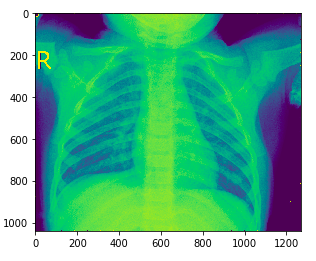
\includegraphics[resolution=100, scale=0.7]{ExampleLungImage.png}
		\caption{Losowy plik z zestawu walidacyjnego.}
\end{figure}

Warto wybrać kilka losowych zdjęć dla potwierdzenia ogólnej poprawności danych. Nie sprawdzi się w ten sposób wszystkich danych, ale pozwoli to na wstępny ogląd z czym się pracuje.

\subsection{Wyniki nauczania}
Kolejnym wspólnym elementem dla każdego z programów głębokiego uczenia maszynowego jest przeglądanie danych wynikowych i analiza przypadków w których sieć gorzej sobie radzi albo radzi sobie nadzwyczaj dobrze. Powszechną praktyką jest samodzielne przejrzenie kilku przykładów następujących kategorii:
\begin{itemize}
\item Kilka losowo wybranych poprawnie sklasyfikowanych odpowiedzi,
\item kilka losowo wybranych niepoprawnie sklasyfikowanych odpowiedzi,
\item odpowiedzi dla każdej z klas z najwyższą pewnością (prawdopodobieństwem) poprawnie sklasyfikowane,
\item odpowiedzi dla każdej z klas z najwyższą pewnością (prawdopodobieństwem) niepoprawnie sklasyfikowanie,
\item odpowiedzi najbardziej niepewne, najbliższe przejścia do innej klasy
\end{itemize}
Wyświetlenie po kilka obrazów z każdej z powyższych kategorii pozwoli zrozumieć dlaczego algorytm zachowuje się w danych sposób i znacząco ułatwia jego modyfikacje. Jak wspomniano we wcześniejszych rozdziałach, uczenie głębokie jest jeszcze praktyką skazaną na metodykę prób i błędów, dlatego wizualizacja jest najprostszym sposobem na uwidocznienie błędów.

\section{Optymalizacja wyników}
\subsection{Wybór stałej uczenia}
Współczynnik uczenia to jeden z najbardziej znaczących hiperparametrów jakie można kontrolować. Definiuje ona tempo aktualizacji parametrów sieci. Jest to jedna z najtrudniejszych wartości do określenia. Do optymalizacji wyników pomocna jest technika opisana przez Leslie N. Smith’a, nazywana cyklicznymi współczynnikami stałej uczenia do trenowania sieci neuronowych (ang. Cyclical Learning Rates for Training Neural Networks). W założeniu technika ta ma całkowicie wyeliminować potrzebę ciągłych eksperymentów w celu znalezienia najlepszych wartości i ustawienia harmonogramu nastawiania globalnych wartości stałej uczenia. Zamiast stale (monotonicznie) obniżać szybkość uczenia się, metoda ta pozwala cyklicznie modyfikować wartość uczenia pomiędzy ustalonymi wartościami krańcowymi minimum i maksimum. Doświadczenie pokazuje (i testy wykonane w publikacji), że trening wykonany osiąga lepszą dokładność klasyfikacji bez potrzeby ręcznego strojenia i to juz w zaledwie kilku iteracjach algorytmu. Technika zmiennych parametrów uczenia potrafi z założenia samodzielnie określić odpowiednie ramy parametrów liniowo zwiększając stopę uczenia przez kilka epok. \cite{DBLP:journals/corr/Smith15a}

\subsection{Sztuczne zwiększenie ilości danych}
Zwiększając ilość epok można dostrzec, że sieć po przekroczeniu pewnej granicy zależnej od ilości posiadanych danych spotyka się z problemem przeuczenia. Oznacza to, że model przestaje uczyć się rozpoznawać konkretne cechy obrazu, a zaczyna wkuwać na pamięć konkretne obrazy ze zbioru treningowego, zatracając umiejętność uogólniania konkretnych klas danych. Doprowadza to do sytuacji kiedy zestaw treningowy jest zapamiętany i rozpoznawany prawidłowo dla każdego obiektu, ale nowe dane, nie spotkane wcześniej przez sieć, są rozpoznawane gorzej niż w przypadku kiedy sieć umiałaby generalizować na podstawie cech obrazu.
Dobrym sposobem na uniknięcie problemu przeuczenia jest dostarczenie większej ilości różnorodnych danych. Technika tworzenia nowych danych z istniejących nazywa się powiększaniem danych (ang. data augumentation). Jest to zaawansowany proces, często pomijany w książkach ze względu na trudności w implementacji i zwyczajowy brak gotowych rozwiązań w najpopularniejszych bibliotekach. 
Proces zwiększania ilości danych w uczeniu maszynowym polega losowej zmianie obrazów w procesie powielania obrazów treningowych. Zmiana jest drobną modyfikacją, nie mającą wpływu na główne cechy w tym ostateczne rozpoznanie obrazu. Najlepszymi operacjami powielającymi dane są:

\begin{itemize}
\item poziome i pionowe odbicie (jeśli odwrócony obraz ma sens np. zdjęcia satelitarne),
\item zbliżanie,
\item obracanie obrazu o kilka stopni (kąt obracania powinien być niewielki).
\end{itemize}

Konwolucyjna sieć neuronowa jest w stanie nauczyć się lepiej rozpoznawać cechy zdjęcia jeśli otrzyma kilka modyfikowanych kopii tego samego obrazu. Należy jednak pamiętać że nie jest to metoda pozwalająca uzyskać setki obiektów uczących z każdego przykładu, tutaj znów ryzykuje się przeuczeniem. Zwyczajowo pięć sztuk z każdego obiektu pozwala zwiększyć znacząco zestaw uczący bez ryzyka przeuczenia. 
Jak widać poniżej na przykładzie architektury ResNet34, dodatnie sztucznie wygenerowanych danych znacząco zwiększyło jakość klasyfikacji, aż o 12,5\%. Niestety metoda nie jest jeszcze powszechnie stosowana, wynika to po części braku styczności z niewielką ilością danych badaczy dużych ośrodków takich jak DeepMind czy Microsoft AI Research. W największych laboratoriach programiści mają do dyspozycji ogromne ilości danych i na żądanie otrzymują zasoby na pozyskanie dodatkowych danych z centrów danych. Z tego powodu technika powielania nie ma odzwierciedlenia w bibliotekach rozwijanych przez duże ośrodki badawcze. 

\subsection{Cykliczny współczynnik uczenia}
Kolejną techniką poprawienia jakości uczenia jest zastosowanie algorytmu gradientu spadkowego z ponownym uruchamianiem. Metoda ta polega na wygaszaniu współczynnika uczenia, zmniejszając jego wartość w trakcie pracy algorytmu. Następnie wykonywana jest operacja próby wyjścia z minimum lokalnego celem znalezienia prawidłowej przestrzeni wag, takiej która będzie cechowała się stabilnością dla większej gamy przykładów, prócz samej dokładności. Znów celem jest generalizowanie rozpoznawanej klasy, a nie uczenie się wszystkich przykładów. \cite{DBLP:journals/corr/HuangLPLHW17}

\section{Analiza wyników}
Najważniejszą miarą wydajności sieci jest wskaźnik jak dobrze klasyfikuje nowe dane. Poważnym błędem jest założenie, że sieć jest w stanie nauczyć się w 100\% rozpoznawać wszystkie elementy. Analiza zawiera trzy parametry, które wykazują w jaki sposób konkretne architektury osiągają najwyższe możliwe osiągi na dostępnym sprzęcie. Należy zaznaczyć iż w przypadku kart graficznych z większą ilością pamięci wyniki znacząco uległyby zmianie. Wynika to z faktu iż cały zestaw uczący jest ładowany do pamięci i w przypadku bardziej rozbudowanych sieci, należy obrazy pierw przeskalować tak by nie otrzymać błędu braku dostępnej pamięci. Dzieje się tak szczególnie często, w trakcie stosowania sztucznego powielania danych.

W tej pracy przyjęto dwa scenariusze reakcji na problem braku pamięci. Pierwszy, zmniejszone zostają rozmiary obrazów do rozdzielczości pozwalającej wszystkim architekturom na wytrenowanie od początku do końca z wszystkimi modyfikacjami algorytmu. Metoda najmniejszego wspólnego mianownika pozwala ocenić skuteczność bez uwzględniania ograniczeń sprzętowych. Drugi scenariusz zakłada największą możliwą rozdzielczość tylko dla podstawowego uczenia sieci nie uwzględniając zasobochłonnego strojenia.

Dla pełnej nauki ze strojeniem (pełnym) określone zostały następujące parametry:
\begin{itemize}
\item Ilość epok: 6, wraz 
\item Krok uczenia: 0,01
\item Rozmiar obrazu wejściowego: ilość pikseli jest zmienna. Ograniczeniem jest ilość parametrów sieci. Dla kompaktowych, takich jak szczątkowe sieci neuronowe, używana karta graficzna jest w stanie przechować nawet obrazy nawet do rozmiaru powyżej 500 pikseli. Dla tych największych, jak DenseNet należy ograniczyć rozmiar sygnału wejściowego do 200 pikseli.
\end{itemize}

Dla podstawowego uczenia sieci bez dodatkowych technik usprawniających model dobrano parametry:
\begin{itemize}
\item Ilość epok: 6
\item Krok uczenia: zmienny, wyliczany algorytmem dla różnych warstw od 0,001 do 1
\item Rozmiar obrazu wejściowego: zmienny dla każdej architektury ustalany indywidualnie wg. maksymalnie możliwego rozmiaru.
\end{itemize}

Wartosci po podstawowym nauczaniu sieci:
\begin{center}
    \begin{tabular}{ | l | l | l | l | l |}
    \hline
    Sieć & Rozmiar wejścia & Dokładność & Błąd treningowy & Błąd walidacyjny \\ \hline
    ResNet34 & 500 & 93,75\% & 6,67\% & 9,31\% \\ \hline
    VGG19 & 350 & 100\%& 8,10\% & 8,10\%\\ \hline
    Wide Residual Network & 350 & 93,75\% & 4,22\% & 25,64\% \\ \hline
    ResNeXt 101 & 350 & 100\%& 4,67\% & 4,86\%\\\hline
    Inception v4 & 350 & 7,46\% & 8,98\% & 93,75\% \\ \hline
    DenseNet 201 & 350 & 100\% & 3,56\% & 3,82\% \\ \hline
    \end{tabular}
\end{center}

Wartości po nauczaniu sieci ze strojeniem:
\begin{center}
    \begin{tabular}{ | l | l | l | l | l |}
    \hline
    Sieć & Rozmiar wejścia & Dokładność & Błąd treningowy & Błąd walidacyjny \\ \hline
    ResNet34 & 300 & 100\% & 5,45\% & 3,22\% \\ \hline
    VGG19 &  &  &  & \\ \hline
    ResNeXt &  &  &  &  \\ \hline
    Inception v4 &  &  &  &  \\ \hline
    DenseNet 201 &  &  &  &  \\ \hline
    \end{tabular}
\end{center}

Trening sieci ze strojeniem jest zadaniem wymagającym sporej dozy cierpliwości. Nie można uruchomić algorymu uczącego z nadzieją na zadowalające wyniki. Rozmiar pamięci potrzebnej na TTA, cykliczne współczynniki uczenia, czy stochastic gradient descent algo with restarts (jak to po polsku nazwać?) wzrasta wielokrotnie z każdą kolejną epoką. Należy dobierać parametry metodą prób i błędów, starając się maksymalnie wykorzystać dostępny sprzęt. Hiperparametry, na które należy zwrócić szczególną uwagę to: rozmiar syngnałów wejściowych, wybrane typy próbkowania przekształceń obrazu (TTA), ilość cykli dla każdej epoki.

\subsection{ResNet} % 300px
ResNet jest architekturą najłatwiejszą do wytrenowania. Jej kompaktowa struktura pozwala zmieścić cały zbiór danych w rozmiarze 500 pikseli. Również po dodaniu sztucznie wygenerowanych danych, niewielka ilość parametrów bez problemu pozwala na trenowanie w ograniczonych pamięciowo środowiskach. Jest to świetna wiadomość dla osób pracujących na pojedynczych maszynach GPU. Wstępne nauczenie sieci dało świetny rezultat widoczny poniżej.

Słowem wyjaśnienia, dokładność sieci na poziomie 100\%, udało się osiągnąć tworząc duży rozmiar sygnału wejściowego, dlatego sieć jest w stanie dokładniej rozróżnić cechy występujące na obrazie. Stosunkowo prosty podział zbioru uczącego na dwie klasy, umożliwia klasyfikację z prostym podziałem płaszczyzny. Domena obrazowania medycznego ma zaletę wyłonienia okreśłonej (zazwyczaj jednej) cechy obrazu bez szumu środowiskowego. Przez szum rozumiane jest otoczenie obrazu (pozostałe przedmioty na scenie), specyficzne ułożenie czy kąt pod jakim został wykonany obraz. Można to porównać do rysowania podziału liczb ujemnych i dodatnich na osi x.
Błąd zestawu walidacyjnego jest niższy ze względu na wiele czynników. Błąd zestawu treningowy jest średnią strat ze wszystkich partii uczących, model zmieniając się w czasie zmniejsza błąd, ale pozostają wpływy z wczesnych etapów uczenia. Drugim aspektem jest mechanizm odrzucania połączeń, aktywny w trakcie uczenia (dla przypomnienia, zapobiega on przeuczeniu sieci). Mechanizm ten jest wyłączony w trakcie walidacji.

\subsection{VGG}

\subsection{ResNeXt}

\subsection{Wide Residual Network}

\subsection{Inception}

\subsection{DenseNet} %na rozmiarze 100 pikseli
Najpopularniejsza architektura dla uczenia zdjęć. Jest bardzo szybka w trenowaniu nowych modeli i posiada implementację w każdej bibliotece głębokiego uczenia. Najlepszy wynik jaki autor zdołał uzyskać:

\subsection{Porównanie czasu uczenia (CPU i GPU)}
Sekcja poświęcona na uświadomienie jak wielka przepaść w czasie uczenia istnieje między uczeniem modelu na procesorze jednostki centralnej komputera, a procesorze jednostki graficznej. Trenowanie obrazów odbywa się tylko na ostatnich warstwach architektury ResNet, ponieważ uczenie całości zajęłoby wiele tygodni na zwykłym komputerze klasy PC.
Oba pomiary dotyczą już przygotowanej sieci z dostrojeniem, a hiperparametry pozostają takie same, jak w najlepszym wyniku uczenia sieci w poprzednich sekcjach. Do pomiaru czasu użyto prostego narzędzia UNIX'owego ''time''.

\begin{center}
    \begin{tabular}{ | l | l | l | l | l |}
    \hline
    Parametr & CPU & GPU & CPU ze strojeniem & GPU ze strojeniem \\ \hline
    Czas & 10,2s & 12,4s & 2612s &  \\ \hline
    Dokładność & 100\% & 93,7\% & 100\% & \\ \hline
    Błąd treningowy & 8,5\% & 8\% & 7,5\% &  \\ \hline
    Błąd walidacyjny & 10,2\% & 10\% & 3,7\% &  \\ \hline
    \end{tabular}
\end{center}

\section{Podsumowanie}
Pierwszym wnioskiem jaki nasuwa się po przeprowadzeniu testów wydajności jest: nie zaczynać przygody z głębokimi sieciami neuronowymi bez dostępu do procesora graficznego ze średniej półki cenowej. Oczekiwanie na wyniki używając jedynie CPU, zniechęci każdego do eksperymentów, a na tym obecnie polega dobieranie świetnych modeli. Wybierając kartę graficzną również należy się kierować odpowiednio dużą pamięcią. Spora część zbioru danych uczących jest ładowana do pamięci GPU, stąd zaleca się minimum 6Gb.

Wpływ wybranej architektury na wynik ma znaczenie, malejące z każdą nową siecią. Zbliżając się do blisko stuprocentowej skuteczności rozpoznawania obrazów, trudno jest stwierdzić że istnieją wyzwania w tej dziedzinie. Należałoby się raczej skupić na bezpieczeństwie sieci i zabezpieczeniami przed próbami oszukania. Ataki stają się popularne, kiedy agenci automatyczni zostają wdrożeni na szeroką skalę.

Dużo ważniejsze od ułożenia kolejnych warstw neuronów okazują się techniki pozwalające optymalizować znajdywanie optymalnego minimum funkcji określającej model. Nowe techniki pojawiające się z każdym miesiącem pozwalają na skuteczne wykorzystanie algorytmu przez osoby nie znające matematyki stojącej za algorytmami głębokiego uczenia.

% ################################
%        PODSUMOWANIE
% ################################

\chapter*{Podsumowanie}
\markboth{}{Podsumowanie}
\addcontentsline{toc}{chapter}{Podsumowanie}
Głębokie sieci neuronowe w ciągu ostatnich kilku lat stały się ogólnodostępnym narzędziem. Wykorzystanie ich zminiło postać z zastosowań naukowych, na bardziej uniwersalne mechanizmy wspierające życie codzienne.

% ################################
%        SPIS RYSUNKÓW
% ################################

\addcontentsline{toc}{chapter}{Spis rysunków}
\listoffigures

% ################################
%        BIBLIOGRAFIA
% ################################

\selectlanguage{polish}
\printbibliography

\end{document}